\cleardoublepage

\pagenumbering{arabic}

\cleardoublepage
\section{Introduction}

[TODO: replace next paragraphs by actual introduction]

We propose to elaborate upon a CGAL Package which implements some
of the state-of-the-art surface reconstruction methods. Priority will
be given to methods which take as input unorganized point sets and
which compute an implicit function, although we leave the room to
Delaunay-based techniques as all building blocks are available in
CGAL. A common implicit function is an approximate distance function
to the input points or to an estimate tangent plane, or an indicator
function.\\


The package will propose an interface to the CGAL Surface Mesh Generator~\cite{mariette06,oudot05},
and we leave the room to other surface contouring techniques such
as the Marching Cubes algorithm~\cite{37422} and its variants (a
user may prefer using his favorite contouring algorithm).\\


The input can be an unorganized point set, possibly with attributes
such as unoriented normals, oriented normals, confidence values. For
piecewise smooth reconstruction, it is also desirable to take not
only one attribute per point, but possibly several ones (for example,
two normals for a point on a sharp edge, or several normals for a
corner, or even a cone of normals). The input can also be a set of
arbitrary cross sections, be they defined by point sets localized
onto well-defined planes, or as polylines.\\


Since reconstruction methods often require to estimate and/or to orient
the normals of a point set, we plan to implement two components devoted
to this task. These components will make use of existing components
such as PCA or Jet fitting.\\


The output can be either an implicit function (ready for evaluation
by any contouring algorithm), or a surface mesh, compatible with the
BGL Graph concept and CGAL polyhedron when 2-manifold, or represented
as a polygon soup otherwise.


The intended audience of this package is researchers, developers or
students developing algorithms around surface reconstruction. We also
target end users and industrial applications.


\chapter{Kernel Representations}
Our object of study is the $d$-dimensional affine Euclidean space. 
Here we are mainly concerned with cases $d=2$ and $d=3$.
Objects in that space are sets of points. A common way to represent 
the points is the use of \ccHtmlNoLinksFrom{Cartesian} coordinates,
which assumes a reference frame (an origin and $d$ orthogonal axes).
In that framework, a point is represented by a $d$-tuple
\ccTexHtml{$(c_0,c_1,\ldots,c_{d-1})$}{<MATH>(c<SUB>0</SUB>,c<SUB>1</SUB>,...,c<SUB>d-1</SUB>)</MATH>},
and so are vectors in the underlying linear space. Each point is 
represented uniquely by such \ccHtmlNoLinksFrom{Cartesian} coordinates.
%An object can then be represented by an equation, that is, it is the 
%set of
%points whose coordinates satisfy the equation. For example, the 
%equation of a
%line is usually given as $ax + by +c = 0$.
%The line can then be represented by three numbers $a$, $b$, $c$.
Another way to represent points is by homogeneous coordinates. In that
framework, a point is represented by a $(d+1)$-tuple
\ccTexHtml{$(h_0,h_1,\ldots,h_d)$}{<MATH>(h<SUB>0</SUB>,h<SUB>1</SUB>,...,h<SUB>d</SUB>)</MATH>}.
Via the formulae
\ccTexHtml{$c_i = h_i/h_d$}{<MATH>c<SUB>i</SUB>=h<SUB>i</SUB>/h<SUB>d</SUB></MATH>},
the corresponding point with \ccHtmlNoLinksFrom{Cartesian} coordinates
\ccTexHtml{$(c_0,c_1,\ldots,c_{d-1})$}{<MATH>(c<SUB>0</SUB>,c<SUB>1</SUB>,...,c<SUB>d-1</SUB>)</MATH>}
can be computed.  Note that homogeneous coordinates are not unique. 
For \ccTexHtml{$\lambda\ne 0$}{<MATH>lambda != 0</MATH>},
the tuples 
\ccTexHtml{$(h_0,h_1,\ldots,h_d)$}{<MATH>(h<SUB>0</SUB>,h<SUB>1</SUB>
,...,h<SUB>d</SUB>)</MATH>}
 and 
\ccTexHtml{$(\lambda\cdot h_0,\lambda\cdot h_1,\ldots,\lambda\cdot 
h_d)$}{<MATH>(lambda  h<SUB>0</SUB>,lambda  h<SUB>1</SUB>,...,lambda  
h<SUB>d</SUB>)</MATH>} represent the
same point.
For a point with \ccHtmlNoLinksFrom{Cartesian} coordinates \ccTexHtml{$(c_0,c_1,\ldots,c_{
d-1})$}{<MATH>(c<SUB>0</SUB>,c<SUB>1</SUB>,...,c<SUB>d-1</SUB>)</MATH>} a
possible homogeneous representation is
\ccTexHtml{$(c_0,c_1,\ldots,c_{d-1},1)$}{<MATH>(c<SUB>0</SUB>,c<SUB>1</SUB>,...,c<SUB>d-1</SUB>,1)</MATH>}.
\ccHtmlNoLinksFrom{Homogeneous} coordinates in fact allow to represent 
objects in a more general space, the projective space
\ccTexHtml{$\P_d$}{<MATH>P<SUB>d</SUB></MATH>}.
In \cgal, we do not compute in projective geometry. Rather, we use 
homogeneous coordinates to avoid division operations,
since the additional coordinate can serve as a common denominator.

\section{Genericity through Parameterization}
Almost all the kernel objects (and the corresponding functions) are
templates with a parameter that allows the user to choose the
representation of the kernel objects. A type that is used as an
argument for this parameter must fulfill certain requirements on 
syntax and semantics. The list of requirements defines an abstract
kernel concept. In \cgal\ such a kernel concept is often also called 
a \emph{representation class} and denoted by \ccc{R}. A representation 
class provides the actual implementations of the kernel objects.
For all kernel objects \ccc{Kernel_object}, the types 
\ccc{CGAL::Kernel_object<R>} and \ccc{R::Kernel_object} are identical.

CGAL offers four families of concrete models for the concept
representation class, two based on the \ccHtmlNoLinksFrom{Cartesian} representation of points
and two based on the homogeneous representation of points. 
The interface of the kernel objects is designed such that it works well
with both \ccHtmlNoLinksFrom{Cartesian} and homogeneous representation, for example, points
in 2D have a constructor with three arguments as well
(the three homogeneous coordinates of the point).
The common interfaces parameterized with a representation class allow
one to develop code independent of the chosen representation. 
We said ``families'' of models, because both families are parameterized too.
A user can choose the number type used to represent the coordinates.

For reasons that will become evident later,
a representation class provides two typenames for number types, 
namely \ccc{R::FT} and \ccc{R::RT}.%
\ccTexHtml{\footnote{The double colon :: is the \CC\ scope operator.}}{}
The type \ccStyle{R::FT} must fulfill the requirements on what is 
called a {\em field type} in \cgal. This roughly means that \ccStyle{R::FT} 
is a type for which  operations $+$, $-$, $*$ and $/$ are defined
with semantics (approximately) corresponding to those of a field in 
a mathematical sense. Note that, strictly speaking, the built-in type 
\ccc{int} does not fullfil the requirements on a field type, since \ccc{int}s
correspond to elements of a ring rather than a field, especially 
operation $/$ is not the inverse of $*$.
The requirements on the type \ccStyle{R::RT} are weaker.
This type must fulfill the requirements on what is called a {\em ring type}
in \cgal. This roughly means that \ccStyle{R::RT} 
is a type for which  operations $+$, $-$, $*$ are defined with semantics
(approximately) corresponding to those of a ring in a mathematical sense. 
A very limited division operation $/$ must be available as well.
It must work for exact (i.e., no remainder) integer divisions only.
Furthermore, both number types should fulfill \cgal's requirements on a
number type. %see  
Note that a ring type is always a field type but not the other way 
round.

\section{Cartesian Kernels}
With \ccc{Cartesian<FieldNumberType>} you can choose \ccHtmlNoLinksFrom{Cartesian} representation 
of coordinates. When you choose \ccHtmlNoLinksFrom{Cartesian} representation you 
have to declare at the same time the type of the coordinates.
A number type used with the \ccc{Cartesian} representation class
should be a {\em field type} as described above.
As mentioned above, the built-in type \ccc{int} is not a field type.
However, for some computations with  \ccHtmlNoLinksFrom{Cartesian} representation, no 
division operation is needed, i.e., 
a {\em ring type} is sufficient in this case.
With \ccc{Cartesian<FieldNumberType>}, both \ccc{Cartesian<FieldNumberType>::FT}
and \ccc{Cartesian<FieldNumberType>::RT} are mapped to number type \ccc{FieldNumberType}.

\ccc{Cartesian<FieldNumberType>} uses reference counting internally to save copying
costs. CGAL also provides \ccc{Simple_cartesian<FieldNumberType>}, a kernel
that uses \ccHtmlNoLinksFrom{Cartesian} representation but no reference counting. 
Debugging is easier with \ccc{Simple_cartesian<FieldNumberType>}, since the coordinates
are stored within the class and hence direct access to the coordinates is
possible.  Depending on the algorithm, it can also be slightly more or less
efficient than \ccc{Cartesian<FieldNumberType>}.
With \ccc{Simple_cartesian<FieldNumberType>}, both \ccc{Simple_cartesian<FieldNumberType>::FT}
and \ccc{Simple_cartesian<FieldNumberType>::RT} are mapped to number type \ccc{FieldNumberType}.

\section{Homogeneous Kernels}
As we mentioned before, homogeneous coordinates permit to avoid 
division operations in numerical computations, since the additional 
coordinate can serve as a common denominator. 
Avoiding divisions can be useful for exact geometric computation. 
With \ccc{Homogeneous<RingNumberType>} you can choose homogeneous representation 
of coordinates with the kernel objects. As for \ccHtmlNoLinksFrom{Cartesian} representation you 
have to declare at the same time the type used to store the homogeneous
coordinates. Since the homogeneous representation allows one to avoid the
divisions, the number type associated with a homogeneous representation class
must be a model for the weaker concept ring type only. However,
some operations provided by this kernel involve division operations, for
example computing squared distances or returning a \ccHtmlNoLinksFrom{Cartesian} coordinate.
To keep the requirements on the number type parameter of \ccc{Homogeneous}
low, the number type \ccStyle{Quotient<RingNumberType>} is used instead.
This number type turns a ring type into a field type. It maintains
numbers as quotients, i.e. a numerator and a denominator. 
Thereby, divisions are circumvented.
With \ccc{Homogeneous<RingNumberType>}, \ccc{Homogeneous<RingNumberType>::FT} is
equal to \ccStyle{Quotient<RingNumberType>} while 
\ccc{Homogeneous<RingNumberType>::RT} is equal to \ccc{RingNumberType}.

\ccc{Homogeneous<RingNumberType>} uses reference counting internally to save
copying costs. CGAL also provides \ccc{Simple_homogeneous<RingNumberType>}, a
kernel that uses \ccHtmlNoLinksFrom{homogeneous} representation but no reference
counting.  Debugging is easier with \ccc{Simple_homogeneous<RingNumberType>},
since the coordinates are stored within the class and hence direct access to
the coordinates is possible.  Depending on the algorithm, it can also be
slightly more or less efficient than \ccc{Homogeneous<RingNumberType>}.
With \ccc{Simple_homogeneous<RingNumberType>},
\ccc{Simple_homogeneous<RingNumberType>::FT} is equal to
\ccStyle{Quotient<RingNumberType>} while
\ccc{Simple_homogeneous<RingNumberType>::RT} is equal to \ccc{RingNumberType}.

\section{Naming conventions}

The use of representation classes not only avoids problems, it
also makes all \cgal\ classes very uniform. They {\bf always} consist of:
\begin{enumerate}
\begin{ccTexOnly}
\itemsep0pt\topsep0pt\partopsep0pt\parskip0pt\parsep0pt
\end{ccTexOnly}

%\item The {\em name space prefix} \ccStyle{}. This avoids name 
%      clashes. It will be dropped as soon as \CC\ compilers support the 
%      concept of name spaces as a feature of the programming language.

\item The {\em capitalized base name} of the geometric object, such as 
      \ccStyle{Point}, \ccStyle{Segment}, \ccStyle{Triangle}.

\item An {\em underscore} followed by the {\em dimension} of the object, 
      for example $\_2$, $\_3$ or $\_d$.

\item A {\em representation class} as parameter, which itself is
      parameterized with a number type, such as \ccStyle{Cartesian<double>} 
      or \ccStyle{Homogeneous<leda_integer>}.
\end{enumerate}

\section{Kernel as a Traits Class}
Algorithms and data structures in the basic library of CGAL are parameterized 
by a traits class that subsumes the objects on which the algorithm or data
structure operates as well as the operations to do so. For most of the 
algorithms and data structures in the basic library you can use a kernel
as a traits class. For some algorithms you even do not have to specify
the kernel; it is detected automatically using the types of the geometric
objects passed to the algorithm. In some other cases, the algorithms 
or data structures needs more than is provided by a kernel. In these
cases, a kernel can not be used as a traits class.

\section{Choosing a Kernel}
If you start with integral \ccHtmlNoLinksFrom{Cartesian} coordinates, many geometric computations
will involve integral numerical values only. Especially, this is true for
geometric computations that evaluate only predicates, which are tantamount to
determinant computations. Examples are triangulation of point sets and 
convex hull computation.
In this case, the \ccHtmlNoLinksFrom{Cartesian} representation is probably the first choice, even
with a ring type. You might use limited precision integer types like
\ccc{int} or \ccc{long}, use \ccc{double} to present your integers (they
have more bits in their mantissa than an \ccc{int} and overflow nicely), or an 
arbitrary precision integer type like the wrapper \ccc{Gmpz} for the
GMP integers, \ccc{leda_integer} or \ccc{MP_Float}. Note, that unless you use
an arbitrary precision ring type, incorrect results might arise due to
overflow. 

If new points are to be constructed, for example
the \ccHtmlNoLinksFrom{intersection} point of two lines, computation of 
\ccHtmlNoLinksFrom{Cartesian} coordinates usually involves divisions, so
you need to use a field type with \ccHtmlNoLinksFrom{Cartesian} representation
or have to switch to homogeneous representation. 
\ccc{double} is a possible, but imprecise field type.
You can also put any ring type into \ccc{Quotient} to get a
field type and put it into \ccc{Cartesian}, but you better put
the ring type into \ccc{Homogeneous}.
\ccc{leda_rational} and \ccc{leda_real} are valid field types, too.

If it is crucial for you that the computation is reliable, 
the right choice are probably number types that guarantee
exact computation. The number type \ccc{leda_real} guarantees
that all decisions and hence all branchings in a computation
are correct. They also allow you to compute approximations to whatever
precision you need. Furthermore computation with 
\ccc{leda_real} is faster than computation with arbitrary precision
arithmetic. So if you would like to avoid surprises caused by imprecise
computation, this is a good choice. In fact, it is a good choice with
both representations, since divisions slow down the computation of
the reals and hence it might pay-off to avoid them.

Still other people will prefer the built-in
type {\tt double}, because they need speed and can live with
approximate results, or even algorithms that, from time to time,
crash or compute incorrect results due to accumulated rounding errors.

\section{Kernel Geometry}

\subsection{Points and Vectors}
In \cgal, we strictly distinguish between points, vectors and directions.
A {\em point} is a point in the Euclidean space
$\E^d$, a {\em vector} is the difference of two points $p_2$, $p_1$
and denotes the direction and the distance from $p_1$ to $p_2$ in the
vector space $\R^d$, and a {\em direction} is a vector where we forget
about its length.
They are different mathematical concepts. For example, they behave
different under affine transformations and an addition of two
points is meaningless in affine geometry.  By putting them in different
classes we not only get cleaner code, but also type checking by the
compiler which avoids ambiguous expressions. Hence, it pays twice to
make this distinction.

\cgal\ defines a symbolic constant \ccStyle{ORIGIN} of type \ccc{Origin}
which denotes the point at the origin. This constant is used in the conversion 
between points and vectors. Subtracting it from a point $p$ results in the 
locus vector of $p$. 

\begin{cprog}
  Point_2< Cartesian<double> >  p(1.0, 1.0), q;
  Vector_2< Cartesian<double> >  v;
  v = p - ORIGIN;
  q = ORIGIN + v;  
  assert( p == q );
\end{cprog} 

In order to obtain the point corresponding to a vector $v$ you simply
have to add $v$ to \ccStyle{ORIGIN}. If you want to determine 
the point $q$ in the middle between two points $p_1$ and $p_2$, you can write%
\footnote{you might call \ccc{midpoint(p_1,p_2)} instead}

\begin{cprog}
  q = p_1 + (p_2 - p_1) / 2.0;
\end{cprog}  

Note that these constructions do not involve any performance overhead for 
the conversion with the currently available representation classes. 

\subsection{Kernel Objects}
Besides points (\ccc{Point_2<Kernel>}, \ccc{Point_3<Kernel>}, \ccc{Point_d<Kernel>}), 
vectors (\ccc{Vector_2<Kernel>}, \ccc{Vector_3<Kernel>}), and 
directions (\ccc{Direction_2<Kernel>}, \ccc{Direction_3<Kernel>}), 
\cgal\ provides lines, rays, segments, planes,
triangles, tetrahedra, iso-rectangles, iso-cuboids, circles and spheres.

Lines  (\ccc{Line_2<Kernel>}, \ccc{Line_3<Kernel>}) in {\cgal} are oriented. In 
two-dimensional space, they induce a partition of the plane
into a positive side and a negative side. 
Any two points on a line induce an \ccHtmlNoLinksFrom{orientation}
of this line. 
A ray (\ccc{Ray_2<Kernel>}, \ccc{Ray_3<Kernel>}) is semi-infinite interval on a line, 
and this line is oriented from the finite endpoint of this interval towards 
any other point in this interval. A segment (\ccc{Segment_2<Kernel>}, 
\ccc{Segment_3<Kernel>}) is a bounded interval on a directed line,
and the endpoints are ordered so that they induce the same direction 
as that of the line.  

Planes are affine subspaces of dimension two in $\E^3$, passing through 
three points, or a point and a line, ray, or segment. 
{\cgal} provides a correspondence between any plane in the ambient 
space $\E^3$ and the embedding of $\E^2$ in that space.
Just like lines, planes are oriented and partition space into a positive side 
and a negative side.
In \cgal, there are no special classes for half-spaces. Half-spaces in 2D and
3D are supposed to be represented by oriented lines and planes, respectively.

Concerning polygons and polyhedra, the kernel provides triangles,
iso-oriented rectangles, iso-oriented cuboids and tetrahedra. 
More complex polygons\footnote{Any sequence of points can be seen as
a (not necessary simple) polygon or polyline. This view is used 
frequently in the basic library as well.}
and polyhedra or polyhedral surfaces can be obtained 
from the basic library (\ccc{Polygon_2}, \ccc{Polyhedron_3}), 
so they are not part of the kernel. 
As with any Jordan curves, triangles, iso-oriented rectangles and circles
separate the plane into two regions, one bounded and one unbounded.  

\subsection{Orientation and Relative Position}
Geometric objects in \cgal\ have member functions that test the
position of a point relative to the object.  Full dimensional objects
and their boundaries are represented by the same type, 
e.g.\ half-spaces and hyperplanes are not distinguished, neither are balls and
spheres and discs and circles. Such objects split the ambient space into two
full-dimensional parts, a bounded part and an unbounded part 
(e.g.\ circles), or two unbounded parts (e.g.\ hyperplanes). By default these
objects are oriented, i.e., one of the resulting parts is called the
positive side, the other one is called the negative side. Both of
these may be unbounded.

For these objects there is a function \ccStyle{oriented_side()} that
determines whether a test point is on the positive side, the negative
side, or on the oriented boundary. These function returns a value of type
\ccc{Oriented_side}.

Those objects that split the space in a bounded and an unbounded part, have
a member function \ccStyle{bounded_side()} with return type
\ccc{Bounded_side}.

If an object is lower dimensional, e.g.\ a triangle in three-dimensional
space or a segment in two-dimensional space, there is only a test whether a
point belongs to the object or not. This member function, which takes a 
point as an argument and returns a Boolean value, is called \ccStyle{has_on()}

\section{Predicates and Constructions}

\subsection{Predicates}
Predicates are at the heart of a geometry kernel. They are basic units
for the composition of geometric algorithms and encapsulate decisions. 
Hence their correctness is crucial for the control flow and hence for
the correctness of an implementation of a geometric algorithm. \cgal\ uses
the term predicate in a generalized sense. Not only components returning a
Boolean value are called predicates but also components returning an 
enumeration type like a \ccc{Comparison_result} or an \ccc{Orientation}.
We say components, because predicates are implemented both as functions and 
function objects (provided by a kernel class).

\cgal\ provides predicates for the \ccHtmlNoLinksFrom{orientation} of point 
sets (\ccc{orientation}, \ccc{leftturn}, \ccc{rightturn}, \ccc{collinear},
\ccc{coplanar}), for comparing points according to some given order, 
especially for comparing \ccHtmlNoLinksFrom{Cartesian} coordinates
(e.g.~\ccc{lexicographically_xy_smaller}), in-circle and in-sphere tests,
and predicates to compare distances.

\subsection{Constructions}
Functions and function objects that generate objects that are neither 
of type \ccc{bool} nor enum types are called constructions.
Constructions involve computation of new numerical values and may be
imprecise due to rounding errors unless a kernel with an exact number type is 
used.

Affine transformations (\ccc{Aff_transformation_2<Kernel>}, 
\ccc{Aff_transformation_3<Kernel>}) allow to generate new object instances under
arbitrary affine transformations. These transformations include translations,
rotations (in 2D only) and scaling. Most of the geometric objects in a
kernel have a member function \ccc{transform(Aff_transformation t)} 
which applies the transformation to the object instance.

{\cgal} also provides a set of functions that detect or compute the 
\ccHtmlNoLinksFrom{intersection}\ccIndexMainItem{intersection}
between objects of the 2D kernel, and many objects in the 3D kernel,
and functions to calculate their 
squared distance\ccIndexMainItem{distance}\ccIndexSubitem{distance}{squared}.
Moreover, some member functions of kernel objects are constructions. 

So there are routines that compute the square of the Euclidean distance, but no
routines that compute the distance itself. Why?
First of all, the two values can be derived from each other quite easily (by
taking the square root or taking the square). So, supplying only the one and
not the other is only a minor inconvenience for the user.
Second, often either value can be used. This is for example the case when
(squared) distances are compared.
Third, the library wants to stimulate the use of the squared distance instead
of the distance. The squared distance can be computed in more cases and the
computation is cheaper.
We do this by not providing the perhaps more natural routine,
The problem of a distance routine is that it needs the \ccStyle{sqrt}
operation.
This has two drawbacks:
\begin{itemize}
\item
The \ccStyle{sqrt} operation can be costly. Even if it is not very costly for
a specific number type and platform, avoiding it is always cheaper.
\item
There are number types on which no \ccStyle{sqrt} operation is defined,
especially integer types and rationals.
\end{itemize}

\subsection{Polymorphic Return Values}
Some functions can return different types of objects. A typical
\CC\ solution to this problem is to derive all possible return
types from a common base class, to return a pointer to this 
class and to perform a dynamic cast on this pointer. The class
\ccc{Object} provides an abstraction.
An object \ccStyle{obj} of the class \ccc{Object} can
represent an arbitrary class. The only operations it provides is
to make copies and assignments, so that you can put them in lists
or arrays. Note that \ccc{Object} is NOT a common base class for the
elementary classes. Therefore, there is no 
automatic conversion from these classes to \ccc{Object}. Rather 
this is done with the global function \ccc{make_object()}. This 
encapsulation mechanism requires the use of
\ccc{object_cast} to access the encapsulated class (a less
efficient way, which is now discouraged, used to be to
use the \ccc{assign} function).

\ccExample
In the following example, the object class is used as return value for the 
\ccHtmlNoLinksFrom{intersection} computation, as there are possibly different return values.

\begin{cprog}
{
    typedef Cartesian<double>  K;
    typedef K::Point_2         Point_2;
    typedef K::Segment_2       Segment_2;

    Segment_2 segment_1, segment_2;

    std::cin >> segment_1 >> segment_2;

    Object obj = intersection(segment_1, segment_2);

    if (const Point_2 *point = object_cast<Point_2>(&obj)) {
        /* do something with *point */
    } else if (const Segment_2 *segment = object_cast<Segment_2>(&obj)) {
        /* do something with *segment*/
    }
\end{cprog}
\ccHtmlLinksOff%
\begin{cprog}
    /*  there was no intersection */
}
\end{cprog}
\ccHtmlLinksOn%


\medskip
The \ccHtmlNoLinksFrom{intersection} routine itself looks roughly as follows:

\begin{cprog}

template < class Kernel >
Object  intersection(Segment_2<Kernel> s1, Segment_2<Kernel> s2)
{
\end{cprog} 
\ccHtmlLinksOff%
\begin{cprog}
    if (/* intersection in a point */ ) {
\end{cprog} 
\ccHtmlLinksOn%
\begin{cprog}
       Point_2<Kernel> p = ... ;
       return make_object(p);
\end{cprog} 
\ccHtmlLinksOff%
\begin{cprog}
    } else if (/* intersection in a segment */ ) {
\end{cprog} 
\ccHtmlLinksOn%
\begin{cprog}
       Segment_2<Kernel> s = ... ;
       return make_object(s);
    }
    return Object();
}
\end{cprog} 

\subsection{Constructive Predicates}
For testing where a point $p$ lies with respect to a plane defined by three
points $q$, $r$ and $s$, one may be tempted to construct the plane
\ccc{Plane_3<Kernel>(q,r,s)} and use the method \ccc{oriented_side(p)}. 
This may pay off if many tests with respect to the plane are made. 
Nevertheless, unless the number type is exact, the constructed plane 
is only approximated, and round-off errors may lead 
\ccc{oriented_side(p)} to return an \ccHtmlNoLinksFrom{orientation} 
which is different from the \ccHtmlNoLinksFrom{orientation} of $p$, $q$, $r$, 
and $s$.

In {\cgal}, we provide predicates in which such
geometric decisions are made directly with a reference to the input points
$p$, $q$, $r$, $s$, without an intermediary object like a plane. 
For the above test, the recommended way to get the result is to use
\ccc{orientation(p,q,r,s)}. For exact number types, the situation is different.
If several tests are to be made with the same
plane, it pays off to construct the plane and to use \ccc{oriented_side(p)}.




\gdef\ccNewRefManualStyle{\ccTrue}
\marginparsep10mm
\marginparwidth15mm
\newcommand{\KernelRefLayout}{\ccTexHtml{%
    \ccSetThreeColumns{const Comparison_result}{}{\hspace*{8cm}}
    \ccPropagateThreeToTwoColumns}{}}

\chapter{Reference Pages}
The following pages give a complete overview on the functionality provided 
in the kernel. \cgal\ componenents and concepts are listed in alphabetical
order.


\KernelRefLayout
%\ccHtmlNoRefLinks
\begin{ccRefFunction}{angle}

\ccHtmlNoLinks
\ccFunction{Angle angle(const Vector_2<Kernel>&u, 
                        const Vector_2<Kernel>&v);}
{returns \ccStyle{OBTUSE}, \ccStyle{RIGHT} or \ccStyle{ACUTE} depending
on the angle formed by the two vectors $u$ and $v$.}

\ccHtmlNoLinks
\ccFunction{Angle angle(const Point_2<Kernel>& p,
                        const Point_2<Kernel>& q,
                        const Point_2<Kernel>& r);}
{returns \ccStyle{OBTUSE}, \ccStyle{RIGHT} or \ccStyle{ACUTE} depending
on the angle formed by the three points $p$, $q$, $r$ ($q$ being the vertex of
the angle). The returned value is the same as \ccc{angle(p - q, r - q)}.}

\ccHtmlNoLinks
\ccFunction{Angle angle(const Point_2<Kernel>& p,
                        const Point_2<Kernel>& q,
                        const Point_2<Kernel>& r,
                        const Point_2<Kernel>& s);}
{returns \ccStyle{OBTUSE}, \ccStyle{RIGHT} or \ccStyle{ACUTE} depending
on the angle formed by the two vectors $pq$, $rs$. The returned value is
the same as \ccc{angle(q - p, s - r)}.}

\ccHtmlNoLinks
\ccFunction{Angle angle(const Point_3<Kernel>& p,
                        const Point_3<Kernel>& q,
                        const Point_3<Kernel>& r);}
{returns \ccStyle{OBTUSE}, \ccStyle{RIGHT} or \ccStyle{ACUTE} depending
on the angle formed by the three points $p$, $q$, $r$ ($q$ being the vertex of
the angle).}

\end{ccRefFunction}


\KernelRefLayout
\begin{ccRefEnum}{Angle}
\ccInclude{CGAL/enum.h}

\ccGlobalEnum{enum Angle {OBTUSE, RIGHT, ACUTE};
}

\ccRefLabel{OBTUSE}  %% add label for table-of-contents in intro.tex.
\ccRefLabel{RIGHT}  %% add label for table-of-contents in intro.tex.
\ccRefLabel{ACUTE}  %% add label for table-of-contents in intro.tex.
\ccHtmlCrossLink{OBTUSE}     %% add further rules for cross referencing links
\ccHtmlCrossLink{RIGHT}     %% add further rules for cross referencing links
\ccHtmlCrossLink{ACUTE}     %% add further rules for cross referencing links

\ccSeeAlso
\ccRefIdfierPage{CGAL::angle} \\
%\ccRefConceptPage{Kernel::Angle_2}\\
%\ccRefConceptPage{Kernel::Angle_3} \\
\end{ccRefEnum}

\KernelRefLayout
\begin{ccRefClass}{Aff_transformation_2<Kernel>}

\ccDefinition
The class \ccRefName\ represents two-dimensional affine transformations. 
The general form of an affine transformation is based on a homogeneous
representation of points. Thereby all transformations can be realized by
matrix multiplications. 

Multiplying the transformation matrix by a scalar does not change the
represented transformation. Therefore, any transformation represented
by a matrix with rational entries can be represented by a
transformation matrix with integer entries as well. (Multiply the
matrix with the common denominator of the rational entries.) Hence, it
is sufficient to use the number type \ccStyle{Kernel::RT} to represent
the entries of the transformation matrix.

{\cgal} offers several specialized affine transformations. Different
constructors are provided to create them. They are parameterized with
a symbolic name to denote the transformation type, followed by
additional parameters. The symbolic name tags solve ambiguities in the
function overloading and they make the code more readable, i.e., what
type of transformation is created.

Since two-dimensional points have three homogeneous coordinates, we
have a $3\times 3$ matrix ${(m_{ij})}_{i,\,j=0\ldots 2}$.

If the homogeneous representations are normalized (the homogenizing
coordinate is 1), then the upper left $2\times 2$ matrix realizes
linear transformations. In the matrix form of a translation, the
translation vector $(v_0,\,v_1,\,1)$ appears in the last column of the
matrix. The entries $m_{20}$ and $m_{21}$ are always zero and
therefore do not appear in the constructors.

\ccCreation
\ccCreationVariable{t}

\ccConstructor{Aff_transformation_2(const Identity_transformation& );}
            {introduces an identity transformation.}

\ccConstructor{Aff_transformation_2(const Translation,
                                    const Vector_2<Kernel> &v);}
            {introduces a translation by a vector $v$.}

\ccConstructor{Aff_transformation_2(const Rotation,
                             const Direction_2<Kernel> &d,
                             const Kernel::RT &num,
                             const Kernel::RT &den = RT(1));}
            {approximates the rotation over the angle indicated by direction 
             $d$, such that the differences between the sines and cosines
             of the rotation given by d and the approximating rotation
             are at most $num/den$ each.
             \ccPrecond $num/den>0$ and $d != 0$. }

\ccConstructor{Aff_transformation_2(const Rotation,
                                       const Kernel::RT &sine_rho, 
                                       const Kernel::RT &cosine_rho, 
                                       const Kernel::RT &hw = RT(1));}
            {introduces a rotation by the angle \ccStyle{rho}.
             \ccPrecond 
             $sine\_rho^2 + cosine\_rho^2 == hw^2$.}

\ccConstructor{Aff_transformation_2(const Scaling,
                                       const Kernel::RT &s,
                                       const Kernel::RT &hw = RT(1));}
            {introduces a scaling by a scale factor $s/hw$.}

\newsavebox{\arrtwo}
\newsavebox{\arrlintwo}
\newsavebox{\transvectwo}

\savebox{\arrtwo}{\small $\left(\begin{array}{ccc}
                 m_{00} & m_{01} & m_{02}\\
                 m_{10} & m_{11} & m_{12}\\
                  0     &  0     & hw
              \end{array}\right)$}

\savebox{\arrlintwo}{\small $\left(\begin{array}{cc}
                 m_{00} & m_{01}\\
                 m_{10} & m_{11}
              \end{array}\right)$}

\savebox{\transvectwo}{\small $\left(\begin{array}{c}
                 m_{02}\\
                 m_{12}
              \end{array}\right)$}

\ccConstructor{Aff_transformation_2(
                const Kernel::RT &m00, const Kernel::RT &m01, const Kernel::RT &m02,
                const Kernel::RT &m10, const Kernel::RT &m11, const Kernel::RT &m12,
                const Kernel::RT &hw = RT(1));}
            {introduces a general affine transformation in the
             \ccTexHtml{$3 \times 3$ matrix form \usebox{\arrtwo}.}%
             {3x3 matrix <IMG ALIGN=CENTER SRC="fig/arrtwo.gif"> .}
             The sub-matrix \ccTexHtml{$1\over hw$\usebox{\arrlintwo}}%
             {<span class="math">hw<SUP>-1</SUP></span> <IMG ALIGN=CENTER 
             SRC="fig/arrlintwo.gif">} contains the scaling and rotation 
             information, the vector \ccTexHtml{$1\over hw$
             \usebox{\transvectwo}}{<span class="math">hw<SUP>-1</SUP></span>
             <IMG ALIGN=CENTER SRC="fig/transvectwo.gif">}
             contains the translational part of the transformation.}

\savebox{\arrtwo}{\small $\left(\begin{array}{ccc}
                 m_{00} & m_{01} & 0\\
                 m_{10} & m_{11} & 0\\
                  0     &  0     & hw
              \end{array}\right)$}
                  
\ccConstructor{Aff_transformation_2(
                                       const Kernel::RT &m00, const Kernel::RT &m01,
                                       const Kernel::RT &m10, const Kernel::RT &m11,
                                       const Kernel::RT &hw = RT(1));}
            {introduces a general linear transformation 
             \ccTexHtml{\usebox{\arrtwo},}{<IMG ALIGN=CENTER 
               SRC="fig/arrtwo2.gif"> ,}
             i.e.\ there is no translational part.}


\ccOperations

The main thing to do with transformations is to apply them on
geometric objects. Each class \ccStyle{Class_2<Kernel>} representing
a geometric object has a member function:

\ccStyle{Class_2<Kernel>  transform(Aff_transformation_2<Kernel> t)}.


The transformation classes provide a member function \ccStyle{transform()}
for points, vectors, directions, and lines:

\ccMethod{Point_2<Kernel>  transform(const Point_2<Kernel> &p) const;}
       {}
\ccGlue
\ccMethod{Vector_2<Kernel>  transform(const Vector_2<Kernel> &p) const;}
       {}
\ccGlue
\ccMethod{Direction_2<Kernel>  transform(const Direction_2<Kernel> &p) const;}
       {}
\ccGlue
\ccMethod{Line_2<Kernel>  transform(const Line_2<Kernel> &p) const;}
       {}

\cgal\ provides function operators for these member functions:

\ccMethod{Point_2<Kernel>  operator()(const Point_2<Kernel> &p) const;}
       {}
\ccGlue
\ccMethod{Vector_2<Kernel>  operator()(const Vector_2<Kernel> &p) const;}
       {}
\ccGlue
\ccMethod{Direction_2<Kernel>  operator()(const Direction_2<Kernel> &p) const;}
       {}
\ccGlue
\ccMethod{Line_2<Kernel>  operator()(const Line_2<Kernel> &p) const;}
       {}

\ccHeading{Miscellaneous}

\ccMethod{Aff_transformation_2<Kernel> operator*(const Aff_transformation_2<Kernel> &s) const;}{composes two affine transformations.}

\ccMethod{Aff_transformation_2<Kernel>  inverse() const;}
       {gives the inverse transformation.}

%\ccMethod{Aff_transformation_2<Kernel>  transpose() const;}
%       {returns the affine transformation defined by transposing
%       the linear transformation in \ccVar\ and setting the
%       translational part to zero.}

\ccMethod{bool                 is_even() const;}
       {returns \ccStyle{true}, if the transformation is not reflecting,
        i.e.\ the determinant of the involved linear transformation is
        non-negative.}

\ccMethod{bool                 is_odd() const;}
       {returns \ccStyle{true}, if the transformation is reflecting.}


%\ccMethod{Aff_transformation_2<Kernel>  general_form() const;}
%       {returns the affine transformation in matrix form.}

The matrix entries of a matrix representation of a 
\ccStyle{Aff_transformation_2<Kernel>}
can be accessed trough the following member functions:

\ccMethod{Kernel::FT          cartesian(int i, int j) const;}
                      {}
\ccGlue
\ccMethod{Kernel::FT          m(int i, int j) const;}
       {returns entry $m_{ij}$ in a matrix representation in which $m_{22}$ is 1.}

\ccMethod{Kernel::RT          homogeneous(int i, int j) const;}
                      {}
\ccGlue
\ccMethod{Kernel::RT          hm(int i, int j) const;}
       {returns entry $m_{ij}$ in some fixed matrix representation.} 


For affine transformations  no I/O operators are defined.

%\ccImplementation
%Depending on the constructor we have different internal representations.
%This approach uses less memory and the transformation can be applied
%faster.
%
%Affine transformations offer no \ccStyle{transform()} member function
%for complex objects because they are defined in terms of  points vectors and 
%directions.  As the internal representation of a complex object
%is private the transformation code should go there.

\ccSeeAlso
\ccc{Identity_transformation}, 
\ccc{Rotation}, 
\ccc{Scaling},
\ccc{Translation} \\
\ccc{rational_rotation_approximation}

\ccExample

\begin{cprog}
  typedef Cartesian<double>        K;
  typedef Aff_transformation_2<K>  Transformation;
  typedef Point_2<K>               Point;
  typedef Vector_2<K>              Vector;
  typedef Direction_2<K>           Direction;

  Transformation rotate(ROTATION, sin(pi), cos(pi));
  Transformation rational_rotate(ROTATION,Direction(1,1), 1, 100);
  Transformation translate(TRANSLATION, Vector(-2, 0));
  Transformation scale(SCALING, 3);

  Point q(0, 1);
  q = rational_rotate(q); 

  Point p(1, 1);

  p = rotate(p); 

  p = translate(p); 

  p = scale(p);
\end{cprog} 

The same would have been achieved with

\begin{cprog}

  Transformation transform = scale * (translate * rotate);
  p = transform(Point(1.0, 1.0));
\end{cprog} 

\ccSeeAlso
\ccRefIdfierPage{CGAL::Aff_transformation_3<Kernel>} \\
\ccRefIdfierPage{CGAL::Identity_transformation} \\
\ccRefIdfierPage{CGAL::Reflection} \\
\ccRefIdfierPage{CGAL::Rotation} \\
\ccRefIdfierPage{CGAL::Scaling} \\
\ccRefIdfierPage{CGAL::Translation} \\

\end{ccRefClass} 


\KernelRefLayout
\begin{ccRefClass}{Aff_transformation_3<R>}

\ccDefinition
The class \ccRefName\ represents three-dimensioanl affine transformations. 
The general form of an affine transformation is based on homogeneous
representation of points. Thereby all transformations can be realized by
matrix multiplication. 

Since the general form is based on the homogeneous representation, a
transformation matrix multiplication by a scalar does not change
the represented transformation. Therefore, any transformation represented
by a matrix with rational entries can be represented by a 
transformation matrix with integer entries as well by multiplying
the matrix with the common denominator of the rational entries. 
Hence it is sufficient to have number type \ccStyle{R::RT} for the entries 
of an affine transformation.

{\cgal} offers several specialized affine transformations. 
Different constructors are provided to create them. 
They are parameterized with a symbolic name to
denote the transformation type, followed by additional parameters.
The symbolic name tags solve ambiguities in the function
overloading and they make the code more readable, i.e.\ what type
of transformation is created.

In three-dimensional space we have a $4\times 4$ matrix ($m_{ij}$).
Entries $m_{30}$, $m_{31}$, and $m_{32}$ are always zero and 
therefore do not appear in the constructors.

\ccCreation
\ccCreationVariable{t}

\ccConstructor{Aff_transformation_3(const Identity_transformation& );}
            {introduces an identity transformation.}


\ccConstructor{Aff_transformation_3(const Translation,
                                    const Vector_3<R> &v);}
            {introduces a translation by a vector $v$.}
 
\ccConstructor{Aff_transformation_3(const Scaling,
                                    const R::RT &s,
                                    const R::RT &hw = RT(1));}
            {introduces a scaling by a scale factor $s/hw$.}

\newsavebox{\arrthree}
\newsavebox{\arrlinthree}
\newsavebox{\transvecthree}

\savebox{\arrthree}{\small $\left(\begin{array}{cccc}
                 m_{00} & m_{01} & m_{02} & m_{03}\\
                 m_{10} & m_{11} & m_{12} & m_{13}\\
                 m_{20} & m_{21} & m_{22} & m_{23}\\
                  0     &  0     &      0 & hw
              \end{array}\right)$}

\savebox{\arrlinthree}{\small $\left(\begin{array}{ccc}
                 m_{00} & m_{01} & m_{02}\\
                 m_{10} & m_{11} & m_{12}\\
                 m_{20} & m_{21} & m_{22}\\
              \end{array}\right)$}

\savebox{\transvecthree}{\small $\left(\begin{array}{c}
                 m_{03}\\
                 m_{13}\\
                 m_{23}
              \end{array}\right)$}

\ccConstructor{Aff_transformation_3(
    const R::RT &m00, const R::RT &m01, const R::RT &m02, const R::RT &m03,
    const R::RT &m10, const R::RT &m11, const R::RT &m12, const R::RT &m13,
    const R::RT &m20, const R::RT &m21, const R::RT &m22, const R::RT &m23,
                const R::RT &hw = RT(1));}
            {introduces a general affine transformation of the matrix
             form \ccTexHtml{\usebox{\arrthree}.}{<IMG ALIGN=CENTER 
             SRC=arrthree.gif> .} The part \ccTexHtml{$1\over hw$
             \usebox{\arrlinthree}}{<MATH><i>hw</i><SUP>-1</SUP></MATH> 
             <IMG ALIGN=CENTER SRC=arrlinthree.gif>}
             defines the scaling and rotational part of the transformation, 
             while the vector \ccTexHtml{$1\over hw$\usebox{\transvecthree}}%
             {<MATH><i>hw</i><SUP>-1</SUP></MATH> <IMG ALIGN=CENTER 
             SRC=transvecthree.gif>} contains the translational part.}

\savebox{\arrthree}{\small $\left(\begin{array}{cccc}
                 m_{00} & m_{01} & m_{02} & 0\\
                 m_{10} & m_{11} & m_{12} & 0\\
                 m_{20} & m_{21} & m_{22} & 0\\
                  0     &  0     &  0     &hw
              \end{array}\right)$}

\ccConstructor{Aff_transformation_3(
                        const R::RT &m00, const R::RT &m01, const R::RT& m02,
                        const R::RT &m10, const R::RT &m11, const R::RT& m12,
                        const R::RT &m20, const R::RT &m21, const R::RT& m22,
                                                      const R::RT &hw = RT(1));}
            {introduces a general linear transformation of the 
             matrix form \ccTexHtml{\usebox{\arrthree},}{<IMG ALIGN=CENTER 
             SRC=arrthree2.gif> ,} i.e.\ an affine transformation without 
             translational part.}


\ccOperations

Each class \ccStyle{Class_3<R>} representing
a geometric object in 3D has a member function:

\ccStyle{Class_3<R>  transform(Aff_transformation_3<R> t)}.


The transformation classes provide a member function \ccStyle{transform()}
for points, vectors, directions, and planes:

\ccMethod{Point_3<R>  transform(const Point_3<R> &p) const;}
       {}
\ccGlue
\ccMethod{Vector_3<R>  transform(const Vector_3<R> &p) const;}
       {}
\ccGlue
\ccMethod{Direction_3<R>  transform(const Direction_3<R> &p) const;}
       {}
\ccGlue
\ccMethod{Plane_3<R>  transform(const Plane_3<R> &p) const;}
       {}

\cgal\ provides four function operators for these member functions:

\ccMethod{Point_3<R>  operator()(const Point_3<R> &p) const;}
       {}
\ccGlue
\ccMethod{Vector_3<R>  operator()(const Vector_3<R> &p) const;}
       {}
\ccGlue
\ccMethod{Direction_3<R>  operator()(const Direction_3<R> &p) const;}
       {}
\ccGlue
\ccMethod{Plane_3<R>  operator()(const Plane_3<R> &p) const;}
       {}


\ccMethod{Aff_transformation_3<R> 
          operator*(const Aff_transformation_3<R> &s) const;}
       {composes two affine transformations.}

\ccMethod{Aff_transformation_3<R>  inverse() const;}
       {gives the inverse transformation.}

%\ccMethod{Aff_transformation_3<R>  transpose() const;}
%       {returns the affine transformation defined by transposing
%       the linear transformation in \ccVar\ and setting the
%       translational part to zero.}

\ccMethod{bool                 is_even() const;}
       {returns \ccStyle{true}, if the transformation is not reflecting,
        i.e.\ the determinant of the involved linear transformation is
        non-negative.}

\ccMethod{bool                 is_odd() const;}
       {returns \ccStyle{true}, if the transformation is reflecting.}


%\ccMethod{Aff_transformation_3<R>  general_form() const;}
%       {returns the affine transformation in matrix form.}

The matrix entries of a matrix representation of a \ccStyle{Aff_transformation_3<R>}
can be accessed trough the following member functions:

\ccMethod{FT          cartesian(int i, int j) const;}
                      {}
\ccGlue
\ccMethod{FT          m(int i, int j) const;}
       {returns entry $m_{ij}$ in a matrix representation in which $m_{33}$ is 1.}

\ccMethod{RT          homogeneous(int i, int j) const;}
                      {}
\ccGlue
\ccMethod{RT          hm(int i, int j) const;}
       {returns entry $m_{ij}$ in some fixed matrix representation.} 

For affine transformations  no I/O operators are defined.

\ccSeeAlso
\ccRefIdfierPage{CGAL::Aff_transformation_2<R>} \\
\ccRefIdfierPage{CGAL::Identity_transformation} \\
\ccRefIdfierPage{CGAL::Reflection} \\
\ccRefIdfierPage{CGAL::Rotation} \\
\ccRefIdfierPage{CGAL::Scaling} \\
\ccRefIdfierPage{CGAL::Translation} \\


\end{ccRefClass} 

\KernelRefLayout
\begin{ccRefFunction}{are_ordered_along_line}

\ccFunction{bool are_ordered_along_line(const Point_2<R> &p, 
                            const Point_2<R> &q, 
                            const Point_2<R> &r);}
         {returns \ccStyle{true}, iff the three points are collinear and 
          \ccStyle{q} lies between \ccStyle{p} and \ccStyle{r}.
          Note that \ccStyle{true} is returned, if \ccStyle{q==p} or
          \ccStyle{q==r}.}

\ccFunction{bool are_ordered_along_line(const Point_3<R> &p, 
                                        const Point_3<R> &q, 
                                        const Point_3<R> &r);}
         {returns \ccStyle{true}, iff the three points are collinear and 
          \ccStyle{q} lies between \ccStyle{p} and \ccStyle{r}.
          Note that \ccStyle{true} is returned, if \ccStyle{q==p} or
          \ccStyle{q==r}.}

\ccSeeAlso
\ccRefIdfierPage{CGAL::are_strictly_ordered_along_line} \\
\ccRefIdfierPage{CGAL::collinear_are_ordered_along_line} \\
\ccRefIdfierPage{CGAL::collinear_are_strictly_ordered_along_line} \\


\end{ccRefFunction}


\KernelRefLayout
\begin{ccRefFunction}{are_strictly_ordered_along_line}

\ccFunction{bool are_strictly_ordered_along_line(const Point_2<Kernel> &p, 
                            const Point_2<Kernel> &q, 
                            const Point_2<Kernel> &r);}
         {returns \ccStyle{true}, iff the three points are collinear and 
          \ccStyle{q} lies strictly between \ccStyle{p} and \ccStyle{r}.
          Note that \ccStyle{false} is returned, if \ccStyle{q==p} or
          \ccStyle{q==r}.}

\ccFunction{bool are_strictly_ordered_along_line(const Point_3<Kernel> &p, 
                                                 const Point_3<Kernel> &q, 
                                                 const Point_3<Kernel> &r);}
         {returns \ccStyle{true}, iff the three points are collinear and 
          \ccStyle{q} lies strictly between \ccStyle{p} and \ccStyle{r}.
          Note that \ccStyle{false} is returned, if \ccStyle{q==p} or
          \ccStyle{q==r}.}

\ccSeeAlso
\ccRefIdfierPage{CGAL::are_ordered_along_line} \\
\ccRefIdfierPage{CGAL::collinear_are_ordered_along_line} \\
\ccRefIdfierPage{CGAL::collinear_are_strictly_ordered_along_line} \\



\end{ccRefFunction}


\KernelRefLayout
\begin{ccRefFunction}{assign}
\ccTexHtml{\ccSetThreeColumns{Orientation}{}{\hspace*{8.5cm}}}{}

\ccInclude{CGAL/Object.h}

\ccFunctionTemplate{T}{template <class T> bool assign(T& c, const Object& o);}
       {assigns \ccStyle{o} to \ccStyle{c} if \ccStyle{o}
        was constructed from an object of type \ccStyle{T}.
        Returns \ccc{true}, if the assignment was possible.}

\ccSeeAlso
\ccRefIdfierPage{CGAL::intersection} \\
\ccRefIdfierPage{CGAL::make_object} \\

\end{ccRefFunction}


\KernelRefLayout
\begin{ccRefClass} {Bbox_2}
\ccInclude{CGAL/Bbox_2.h}

\ccDefinition  An object \ccStyle{b} of the class \ccRefName\ is a bounding 
box in the two-dimensional Euclidean plane $\E^2$. This class is not templated.

\ccCreation
\ccCreationVariable{b}

\ccConstructor{Bbox_2(double x_min, double y_min,
                      double x_max, double y_max);}
            {introduces a bounding box \ccVar\ with lower left corner at 
             \ccStyle{(xmin, ymin)} and with upper right corner at 
             \ccStyle{(xmax, ymax)}.}


\ccOperations

\ccHidden\ccMethod{bool operator==(const Bbox_2 &c) const;}
       {Test for equality.}

\ccHidden\ccMethod{bool operator!=(const Bbox_2 &q) const;}
       {Test for inequality.}

\ccMethod{double                 xmin() const;}{}
\ccGlue
\ccMethod{double                 ymin() const;}{}
\ccGlue
\ccMethod{double                 xmax() const;}{}
\ccGlue
\ccMethod{double                 ymax() const;}{}

\ccMethod{Bbox_2              operator+(const Bbox_2 &c) const;}
       {returns a bounding box of \ccVar\ and \ccStyle{c}.}

\ccSeeAlso
\ccRefIdfierPage{CGAL::Bbox_3} \\
\ccRefIdfierPage{CGAL::do_overlap} \\

\end{ccRefClass} 

\KernelRefLayout
\begin{ccRefClass} {Bbox_3}

\ccInclude{CGAL/Bbox_3.h}

\ccDefinition  An object \ccStyle{b} of the class \ccRefName\ is a bounding 
box in the three-dimensional Euclidean space $\E^3$. 

\ccCreation
\ccCreationVariable{b}


\ccConstructor{Bbox_3(double x_min, double y_min, double z_min,
                         double x_max, double y_max, double z_max);}
            {introduces a bounding box \ccVar\ with lexicographically
	     smallest corner point at \ccStyle{(xmin, ymin, zmin)} 
	     lexicographically largest corner point at 
	     \ccStyle{(xmax, ymax, zmax)}.}


\ccOperations

\ccHidden\ccMethod{bool operator==(const Bbox_3 &c) const;}
       {Test for equality.}

\ccHidden\ccMethod{bool operator!=(const Bbox_3 &q) const;}
       {Test for inequality.}

\ccMethod{double                 xmin() const;}
       {}
\ccGlue
\ccMethod{double                 ymin() const;}
       {}
\ccGlue
\ccMethod{double                 zmin() const;}
       {}
\ccGlue
\ccMethod{double                 xmax() const;}
       {}
\ccGlue
\ccMethod{double                 ymax() const;}
       {}
\ccGlue
\ccMethod{double                 zmax() const;}
       {}


\ccMethod{Bbox_3              operator+(const Bbox_3 &c) const;}
       {returns a bounding box of \ccVar\ and \ccStyle{c}.}

\ccSeeAlso
\ccRefIdfierPage{CGAL::Bbox_2} \\
\ccRefIdfierPage{CGAL::do_overlap} \\


\end{ccRefClass} 

\KernelRefLayout
\begin{ccRefEnum}{Bounded_side}
\ccInclude{CGAL/enum.h}

\ccGlobalEnum{enum Bounded_side {ON_UNBOUNDED_SIDE, ON_BOUNDARY, ON_BOUNDED_SIDE};
}

\ccRefLabel{ON_UNBOUNDED_SIDE}  %% add label for table-of-contents in intro.tex.
\ccRefLabel{ON_BOUNDED_SIDE}  %% add label for table-of-contents in intro.tex.
\ccRefLabel{ON_BOUNDARY}  %% add label for table-of-contents in intro.tex.
\ccHtmlCrossLink{ON_UNBOUNDED_SIDE}     %% add further rules for cross referencing links
\ccHtmlCrossLink{ON_BOUNDED_SIDE}     %% add further rules for cross referencing links
\ccHtmlCrossLink{ON_BOUNDARY}     %% add further rules for cross referencing links
\ccHtmlIndexC[enum_tags]{ON_UNBOUNDED_SIDE} %% add further index entries
\ccHtmlIndexC[enum_tags]{ON_BOUNDED_SIDE} %% add further index entries
\ccHtmlIndexC[enum_tags]{ON_BOUNDARY} %% add further index entries

%\ccSeeAlso
%\ccRefConceptPage{Kernel::HasOnBoundedSide_2} \\
%\ccRefConceptPage{Kernel::HasOnBoundedSide_3} \\

\end{ccRefEnum}

\KernelRefLayout
\begin{ccRefClass}{Cartesian<FieldNumberType>}
\ccInclude{CGAL/Cartesian.h}

\ccDefinition
A model for a \ccc{Kernel} using Cartesian coordinates to represent the
geometric objects.

\ccRefines
\ccc{Kernel}

\ccTypes
\ccTypedef{typedef FieldNumberType FT;}{}
\ccGlue
\ccTypedef{typedef FieldNumberType RT;}{}

\ccImplementation
This model of a kernel uses reference counting.

\ccSeeAlso
\ccc{Simple_cartesian<FieldNumberType>}, \ccc{Homogeneous<RingNumberType>}
\end{ccRefClass}

\KernelRefLayout
\begin{ccRefClass}{Cartesian_converter<K1, K2,
                             Converter = NT_converter<K1::FT, K2::FT> >}
%\ccTexHtml{\ccSetThreeColumns{Point_2< us<RT> > }{}{\hspace*{8.5cm}}}{}

\KernelRefLayout\gdef\ccTagOperatorLayout{\ccFalse}

\ccDefinition

\ccClassTemplateName converts objects from the kernel traits \ccc{K1} to
the kernel traits \ccc{K2}.  Those traits must be of the form
\ccc{Cartesian<FT1>} and \ccc{Cartesian<FT2>} (or the equivalent with
\ccc{Simple_cartesian}).  It then provides the following operators to convert
objects from \ccc{K1} to \ccc{K2}.

\ccInclude{CGAL/Cartesian_converter.h}

\ccTypes

The third template parameter \ccc{Converter} is a function object that must
satisfy:

\ccMemberFunction{K2::FT operator()(const K1::FT &n);}
{ converts \ccc{n} to an \ccc{K2::FT} which has the same value.}

The default value of this parameter uses the conversion operator from
\ccc{K1::FT} to \ccc{K2::FT}.

\ccCreation
\ccCreationVariable{conv}

\ccConstructor{Cartesian_converter<K1, K2, Converter>();}{Default constructor.}

\ccOperations

\ccMemberFunction{K2::Point_2 operator()(const K1::Point_2&p);}
{ returns a \ccc{K2::Point_2} which coordinates are those of \ccc{p},
converted by \ccc{Converter}.}

Similar operators are defined for the other kernel traits types \ccc{Point_3},
\ccc{Vector_2}...


%\ccTexHtml{\KernelRefLayout}{}
\end{ccRefClass}


\KernelRefLayout
\begin{ccRefFunction}{cartesian_to_homogeneous}
\ccTexHtml{\ccSetThreeColumns{Point_2< Homogeneous<RT> > }{}{\hspace*{8.5cm}}}{}

\ccInclude{CGAL/cartesian_homogeneous_conversion.h}

\ccFunction{Point_2< Homogeneous<RT> >
cartesian_to_homogeneous(const Point_2< Cartesian<RT> >& cp);}
        {converts 2d point \ccStyle{cp} with Cartesian representation  
         into a 2d point with homogeneous representation with the same
         number type.}

\ccFunction{Point_3< Homogeneous<RT> >
cartesian_to_homogeneous(const Point_3< Cartesian<RT> >& cp);}
        {converts 3d point \ccStyle{cp} with Cartesian representation  
         into a 3d point with homogeneous representation with the same
         number type.}

\ccTexHtml{\KernelRefLayout}{}

\ccSeeAlso
\ccRefIdfierPage{CGAL::Cartesian<FieldNumberType>} \\
\ccRefIdfierPage{CGAL::Cartesian_converter<K1, K2, NTConverter>} \\
\ccRefIdfierPage{CGAL::Homogeneous<RingNumberType>} \\
\ccRefIdfierPage{CGAL::Homogeneous_converter<K1, K2, RTConverter, FTConverter>} \\
\ccRefIdfierPage{CGAL::homogeneous_to_cartesian} \\
\ccRefIdfierPage{CGAL::homogeneous_to_quotient_cartesian} \\
\ccRefIdfierPage{CGAL::quotient_cartesian_to_homogeneous} \\
\ccRefIdfierPage{CGAL::Simple_cartesian<FieldNumberType>} \\
\ccRefIdfierPage{CGAL::Simple_homogeneous<RingNumberType>} \\

\end{ccRefFunction}


\KernelRefLayout
\begin{ccRefFunction}{centroid}

\ccFunction{Point_2<Kernel>
centroid( const Point_2<Kernel>& p,
          const Point_2<Kernel>& q,
          const Point_2<Kernel>& r);}
 {compute the centroid of the points $p$, $q$, and $r$.}

\ccFunction{Point_2<Kernel>
centroid( const Point_2<Kernel>& p,
          const Point_2<Kernel>& q,
          const Point_2<Kernel>& r,
          const Point_2<Kernel>& s);}
 {compute the centroid of the points $p$, $q$, $r$, and $s$.}

\ccFunction{Point_2<Kernel>
centroid( const Triangle_2<Kernel>& t);}
 {compute the centroid of the triangle $t$.}

\ccFunction{Point_3<Kernel>
centroid( const Point_3<Kernel>& p,
          const Point_3<Kernel>& q,
          const Point_3<Kernel>& r);}
 {compute the centroid of the points $p$, $q$, and $r$.}

\ccFunction{Point_3<Kernel>
centroid( const Point_3<Kernel>& p,
          const Point_3<Kernel>& q,
          const Point_3<Kernel>& r,
          const Point_3<Kernel>& s);}
 {compute the centroid of the points $p$, $q$, $r$, and $s$.}

\ccFunction{Point_3<Kernel>
centroid( const Triangle_3<Kernel>& t);}
 {compute the centroid of the triangle $t$.}

\ccFunction{Point_3<Kernel>
centroid( const Tetrahedron_3<Kernel>& t);}
 {compute the centroid of the tetrahedron $t$.}

\ccSeeAlso
\ccRefIdfierPage{CGAL::barycenter}

\end{ccRefFunction}

\KernelRefLayout
\begin{ccRefClass}{Circle_2<R>}

\ccDefinition

An object of type \ccRefName\ is a circle in the
two-dimensional Euclidean plane $\E^2$. The circle is oriented, i.e.\ 
its boundary has clockwise or counterclockwise \ccHtmlNoLinksFrom{orientation}. The
boundary splits $\E^2$ into a positive and a negative side, where the
positive side is to the left of the boundary. The boundary further
splits $\E^2$ into a bounded and an unbounded side. Note that the
circle can be degenerated, i.e.\ the squared radius may be zero.


% -----------------------------------------------------------------------------
\ccCreation
\ccCreationVariable{c}

\ccHidden
\ccConstructor{ Circle_2( );}{
        introduces an uninitialized variable \ccVar\ of type
        \ccClassTemplateName.}

\ccConstructor{ Circle_2( Point_2<R>  const& center, 
                               R::FT  const& squared_radius,
                               Orientation const& ori = COUNTERCLOCKWISE);}{
        introduces a variable \ccVar\ of type \ccClassTemplateName.
        It is initialized to the circle with center \ccc{center},
        squared radius \ccc{squared_radius} and \ccHtmlNoLinksFrom{orientation}
        \ccc{ori}.
        \ccPrecond \ccc{ori} $\neq$ \ccc{COLLINEAR}, and further,
                   \ccc{squared_radius} $\geq$ 0.}

\ccConstructor{ Circle_2( Point_2<R> const& p,
                          Point_2<R> const& q,
                          Point_2<R> const& r);}{
        introduces a variable \ccVar\ of type \ccClassTemplateName.
        It is initialized to the unique circle which passes through
        the points \ccc{p}, \ccc{q} and \ccc{r}. The \ccHtmlNoLinksFrom{orientation} of
        the circle is the \ccHtmlNoLinksFrom{orientation} of the point triple \ccc{p},
        \ccc{q}, \ccc{r}.
        \ccPrecond \ccc{p}, \ccc{q}, and \ccc{r} are not collinear.}

\ccConstructor{ Circle_2( Point_2<R>  const& p, 
                               Point_2<R>  const& q,
                               Orientation const& ori 
                                                    = COUNTERCLOCKWISE);}{
        introduces a variable \ccVar\ of type \ccClassTemplateName.
        It is initialized to the circle with diameter 
        $\ccTexHtml{\overline{pq}}{pq}$
        and \ccHtmlNoLinksFrom{orientation} \ccc{ori}.
        \ccPrecond \ccc{ori} $\neq$ \ccc{COLLINEAR}.}

\ccConstructor{ Circle_2( Point_2<R>  const& center,
                               Orientation const& ori
                                                    = COUNTERCLOCKWISE);}{
        introduces a variable \ccVar\ of type \ccClassTemplateName.
        It is initialized to the circle with center \ccc{center}, squared
        radius zero and \ccHtmlNoLinksFrom{orientation} \ccc{ori}.
        \ccPrecond \ccc{ori} $\neq$ \ccc{COLLINEAR}.
        \ccPostcond \ccVar.\ccc{is_degenerate()} = \ccc{true}.}

\ccHidden
\ccConstructor{ Circle_2( Circle_2<R> const&);}{
        copy constructor.}

\ccHidden
\ccMemberFunction{ Circle_2<R>& operator = ( Circle_2<R> const&);}{
        assignment.}

% -----------------------------------------------------------------------------
\ccAccessFunctions

\ccMemberFunction{Point_2<R> const& center( ) const;}{
        returns the center of \ccVar.}
\ccGlue
\ccMemberFunction{ R::FT const& squared_radius( ) const;}{
        returns the squared radius of \ccVar.}
\ccGlue
\ccMemberFunction{ Orientation const& orientation( ) const;}{
        returns the \ccHtmlNoLinksFrom{orientation} of \ccVar.}

% -----------------------------------------------------------------------------

\ccHidden\ccMemberFunction{ bool operator == ( Circle_2<R> const& circle2) const;}{
        returns \ccc{true}, iff \ccVar\ and \ccc{circle2} are equal,
        i.e.\ if they have the same center, same squared radius and
        same \ccHtmlNoLinksFrom{orientation}.}

\ccHidden\ccMemberFunction{ bool operator != ( Circle_2<R> const& circle2) const;}{
        returns \ccc{true}, iff \ccVar\ and \ccc{circle2} are not equal.}

% -----------------------------------------------------------------------------
\ccPredicates

\ccMemberFunction{ bool is_degenerate( ) const;}{
        returns \ccc{true}, iff \ccVar\ is degenerate, i.e.\
        if \ccVar\ has squared radius zero.}

\ccMemberFunction{ Oriented_side
                   oriented_side( Point_2<R> const& p) const;}{
        returns either the constant \ccc{ON_ORIENTED_BOUNDARY}, 
        \ccc{ON_POSITIVE_SIDE}, or \ccc{ON_NEGATIVE_SIDE},
        iff \ccc{p} lies on the boundary, properly on the
        positive side, or properly on the negative side
        of \ccVar, resp.}

\ccMemberFunction{ Bounded_side
                   bounded_side( Point_2<R> const& p) const;}{
        returns \ccc{ON_BOUNDED_SIDE},
        \ccc{ON_BOUNDARY}, or \ccc{ON_UNBOUNDED_SIDE}
        iff \ccc{p} lies properly inside, on the boundary, or properly
        outside of \ccVar, resp.}

%\ccMemberFunction{ bool has_on_positive_side( Point const& p) const;}{
%        returns \ccc{true}, iff \ccc{p} lies properly on the
%        positive side of \ccVar.}
%
%\ccMemberFunction{ bool has_on_negative_side( Point const& p) const;}{
%        returns \ccc{true}, iff \ccc{p} lies properly on the
%        negative side of \ccVar.}
%
%\ccMemberFunction{ bool has_on_boundary( Point const& p) const;}{
%        returns \ccc{true}, iff \ccc{p} lies on the boundary
%        of \ccVar.}
%
%\ccMemberFunction{ bool has_on_bounded_side( Point const& p) const;}{
%        returns \ccc{true}, iff \ccc{p} lies properly inside \ccVar.}
%
%\ccMemberFunction{ bool
%                   has_on_unbounded_side( Point const& p) const;}{
%        returns \ccc{true}, iff \ccc{p} lies properly outside of \ccVar.}
\ccMethod{bool has_on_positive_side(const Point_2<R> &p) const;}
       {}
\ccGlue
\ccMethod{bool has_on_negative_side(const Point_2<R> &p) const;}
       {}
\ccGlue
\ccMethod{bool has_on_boundary(const Point_2<R> &p) const;}
       {}
\ccGlue
\ccMethod{bool has_on_bounded_side(const Point_2<R> &p) const;}
       {} 
\ccGlue
\ccMethod{bool has_on_unbounded_side(const Point_2<R> &p) const;}
       {}

% -----------------------------------------------------------------------------
\ccHeading{Miscellaneous}

\ccMemberFunction{ Circle_2<R> opposite() const;}{
        returns the circle with the same center and squared radius as
        \ccVar\, but with \ccHtmlNoLinksFrom{opposite} \ccHtmlNoLinksFrom{orientation}.}


\ccMemberFunction{ Circle_2<R> orthogonal_transform(
                       Aff_transformation_2<R> const& at) const;}{
        returns the circle obtained by applying $at$ on \ccVar.
        \ccPrecond \ccc{at} is an orthogonal transformation.}

\ccMemberFunction{ Bbox_2 bbox() const;}{
        returns a bounding box containing \ccVar.}

\ccSeeAlso

\ccRefConceptPage{Kernel::Circle_2} \\

\end{ccRefClass}

\KernelRefLayout
\begin{ccRefFunction}{circumcenter}

\ccFunction{Point_2<R>
circumcenter( const Point_2<R>& p,
              const Point_2<R>& q,
              const Point_2<R>& r);}
 {compute the center of the circle passing through the points $p$, $q$, and $r$.
  \ccPrecond $p$, $q$, and $r$ are not collinear.}

\ccFunction{Point_3<R>
circumcenter( const Point_3<R>& p,
              const Point_3<R>& q,
              const Point_3<R>& r);}
 {compute the center of the circle passing through the points $p$, $q$, and $r$.
  \ccPrecond $p$, $q$, and $r$ are not collinear.}

\ccFunction{Point_3<R>
circumcenter( const Point_3<R>& p,
              const Point_3<R>& q,
              const Point_3<R>& r,
              const Point_3<R>& s);}
 {compute the center of the sphere passing through the points $p$, $q$, $r$, and $s$.
  \ccPrecond $p$, $q$, $r$, and $s$ are not coplanar.}
\end{ccRefFunction}


\KernelRefLayout
\begin{ccRefConstant}{CLOCKWISE}
\ccGlobalVariable{const Orientation CLOCKWISE = NEGATIVE;}

\ccSeeAlso
\ccRefIdfierPage{CGAL::COUNTERCLOCKWISE} \\

\end{ccRefConstant}

\KernelRefLayout
\begin{ccRefFunction}{cmp_dist_to_point}

\ccFunction{Comparison_result
cmp_dist_to_point(const Point_2<R>& p,
                  const Point_2<R>& q,
                  const Point_2<R>& r);}
          {compares the distances of points \ccStyle{q} and
           \ccStyle{r} to point \ccStyle{p}.
          returns \ccStyle{SMALLER}, iff \ccStyle{q} is closer
          to \ccStyle{p} than \ccStyle{r}, \ccStyle{LARGER}, iff
          \ccStyle{r} is closer to \ccStyle{p} than \ccStyle{q}, and
          \ccStyle{EQUAL} otherwise.}

\ccFunction{Comparison_result
cmp_dist_to_point(const Point_3<R>& p,
                  const Point_3<R>& q,
                  const Point_3<R>& r);}
          {compares the distances of points \ccStyle{q} and
           \ccStyle{r} to point \ccStyle{p}.
          returns \ccStyle{SMALLER}, iff \ccStyle{q} is closer
          to \ccStyle{p} than \ccStyle{r}, \ccStyle{LARGER}, iff
          \ccStyle{r} is closer to \ccStyle{p} than \ccStyle{q}, and
          \ccStyle{EQUAL} otherwise.}
\end{ccRefFunction}


\KernelRefLayout
\begin{ccRefFunction}{cmp_signed_dist_to_line}

\ccFunction{Comparison_result
cmp_signed_dist_to_line(const Line_2<R>&  l,
                        const Point_2<R>& p,
                        const Point_2<R>& q);}
          {returns \ccStyle{LARGER}
           iff the signed distance of \ccStyle{p} and 
           \ccStyle{l} is larger than the signed distance of \ccStyle{q}
           and \ccStyle{l}, \ccStyle{SMALLER}, iff it is smaller,
           and \ccStyle{EQUAL} iff both are equal.}

\ccFunction{Comparison_result
cmp_signed_dist_to_line(const Point_2<R>& p,
                        const Point_2<R>& q,
                        const Point_2<R>& r,
                        const Point_2<R>& s);}
	{returns \ccStyle{LARGER}
	iff the signed distance of \ccStyle{r} and 
	\ccStyle{l} is larger than the signed distance of \ccStyle{s}
	and \ccStyle{l}, \ccStyle{SMALLER}, iff it is smaller,
	and \ccStyle{EQUAL} iff both are equal, where 
        \ccc{l} is the directed line through \ccc{p} and \ccc{q}.}
\end{ccRefFunction}


\KernelRefLayout
\begin{ccRefFunction}{cmp_signed_dist_to_plane}

\ccFunction{Comparison_result
cmp_signed_dist_to_plane(const Plane_3<R>& h,
                         const Point_3<R>& p,
                         const Point_3<R>& q);}
          {returns \ccStyle{LARGER}
           iff the signed distance of \ccStyle{p} and 
           \ccStyle{h} is larger than the signed distance of \ccStyle{q}
           and \ccStyle{h}, \ccStyle{SMALLER}, iff it is smaller,
           and \ccStyle{EQUAL} iff both are equal.}

\ccFunction{Comparison_result
cmp_signed_dist_to_plane(const Point_3<R>& p,
                         const Point_3<R>& q,
                         const Point_3<R>& r,
                         const Point_3<R>& s,
                         const Point_3<R>& t);}
          {returns \ccStyle{LARGER}
           iff the signed distance of \ccStyle{s} and 
           \ccStyle{h} is larger than the signed distance of \ccStyle{t}
           and \ccStyle{h}, \ccStyle{SMALLER}, iff it is smaller,
           and \ccStyle{EQUAL} iff both are equal, where
           \ccc{h} is the oriented plane through \ccc{p}, \ccc{q} and
           \ccc{r}.}
         {}
\end{ccRefFunction}


\KernelRefLayout
\begin{ccRefConstant}{COLLINEAR}
\ccGlobalVariable{const Orientation COLLINEAR = ZERO;}

\ccSeeAlso
\ccRefIdfierPage{CGAL::LEFTTURN} \\
\ccRefIdfierPage{CGAL::RIGHTTURN} \\
\end{ccRefConstant}

\KernelRefLayout
\begin{ccRefFunction}{collinear}
\ccInclude{CGAL/predicates_on_points_2.h}

\ccFunction{bool collinear(const Point_2<R> &p, 
                           const Point_2<R> &q, 
                           const Point_2<R> &r);}
{returns \ccStyle{true}, iff $p$, $q$, and $r$ are collinear.}

\ccInclude{CGAL/predicates_on_points_3.h}

\ccFunction{bool collinear(const Point_3<R> &p,
                           const Point_3<R>&q,
                           const Point_3<R>&r);}
{returns \ccStyle{true}, iff $p$, $q$, and $r$ are collinear.}
\end{ccRefFunction}


\KernelRefLayout
\begin{ccRefFunction}{collinear_are_ordered_along_line}

\ccFunction{bool collinear_are_ordered_along_line(const Point_2<R> &p,
                                      const Point_2<R> &q,
                                      const Point_2<R> &r);}
         {returns \ccStyle{true}, iff \ccStyle{q} lies between \ccStyle{p} 
          and \ccStyle{r}. \ccPrecond \ccStyle{p, q} and \ccStyle{r} are 
          collinear.}

\ccFunction{bool collinear_are_ordered_along_line(const Point_3<R> &p,
                                                  const Point_3<R> &q,
                                                  const Point_3<R> &r);}
         {returns \ccStyle{true}, iff \ccStyle{q} lies between \ccStyle{p} 
          and \ccStyle{r}. \ccPrecond \ccStyle{p, q} and \ccStyle{r} are 
          collinear.}

\ccSeeAlso
\ccRefIdfierPage{CGAL::are_ordered_along_line} \\
\ccRefIdfierPage{CGAL::are_strictly_ordered_along_line} \\
\ccRefIdfierPage{CGAL::collinear_are_strictly_ordered_along_line} \\

\end{ccRefFunction}


\KernelRefLayout
\begin{ccRefFunction}{collinear_are_strictly_ordered_along_line}

\ccFunction{bool collinear_are_strictly_ordered_along_line(const Point_2<Kernel> &p,
                                      const Point_2<Kernel> &q,
                                      const Point_2<Kernel> &r);}
         {returns \ccStyle{true}, iff \ccStyle{q} lies strictly between 
          \ccStyle{p} and \ccStyle{r}. \ccPrecond{\ccStyle{p, q} and \ccStyle{r} are 
          collinear.}}

\ccFunction{bool collinear_are_strictly_ordered_along_line(
                                      const Point_3<Kernel> &p,
                                      const Point_3<Kernel> &q,
                                      const Point_3<Kernel> &r);}
         {returns \ccStyle{true}, iff \ccStyle{q} lies strictly between \ccStyle{p} 
          and \ccStyle{r}. \ccPrecond{\ccStyle{p, q} and \ccStyle{r} are 
          collinear.}}

\ccSeeAlso

\ccRefIdfierPage{CGAL::are_ordered_along_line} \\
\ccRefIdfierPage{CGAL::are_strictly_ordered_along_line} \\
\ccRefIdfierPage{CGAL::collinear_are_ordered_along_line} \\

\end{ccRefFunction}


\KernelRefLayout
\begin{ccRefFunction}{compare_lexicographically_xy}

\ccFunction{Comparison_result
compare_lexicographically_xy(const Point_2<R>& p,
                             const Point_2<R>& q);}
      {Compares the Cartesian coordinates of points \ccStyle{p} and
       \ccStyle{q} lexicographically in $xy$ order: first 
       $x$-coordinates are compared, if they are equal, $y$-coordinates
       are compared.}
\end{ccRefFunction}


\KernelRefLayout
\begin{ccRefFunction}{compare_lexicographically_xyz}

\ccFunction{Comparison_result
compare_lexicographically_xyz(const Point_3<R>& p,
                              const Point_3<R>& q);}
      {Compares the Cartesian coordinates of points \ccStyle{p} and
       \ccStyle{q} lexicographically in $xyz$ order: first 
       $x$-coordinates are compared, if they are equal, $y$-coordinates
       are compared, and if both $x$- and $y$- coordinate are equal,
       $z$-coordinates are compared.}
\end{ccRefFunction}


\KernelRefLayout
\begin{ccRefFunction}{compare_x}

Depending on which \cgal\ \ccHtmlNoLinksFrom{kernel} is used,
different versions of this global function are available. This is
described below.

%%%%%%%%%%%%%%%%%%%%%%%%%%%%%%%%%%%%%%%%%%%%%%
\paragraph{With the basic 2D and 3D Kernel} (see Chapter~\ref{chapter-kernel-23})

\ccFunction{Comparison_result compare_x(const Point_2<Kernel> &p,
                                        const Point_2<Kernel> &q);}
        {compares the $x$-coordinates of $p$ and $q$.}

\ccFunction{Comparison_result compare_x(const Point_3<Kernel> &p,
                                        const Point_3<Kernel> &q);}
        {compares the $x$-coordinates of $p$ and $q$.}

\begin{ccTexOnly}
\begin{figure}[hb]
\centerline{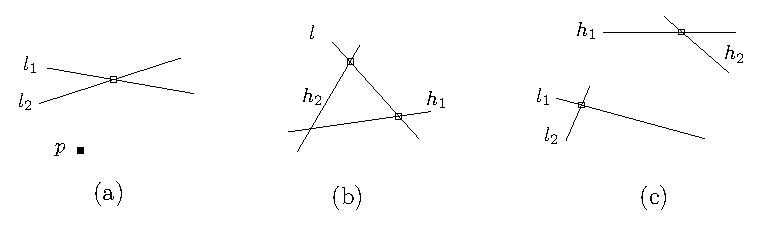
\includegraphics{Kernel_23_ref/fig/compare1}}
\caption{Comparison of the $x$ or $y$-coordinates of the (implicitly
given) points in the boxes.\label{fig-compare}}
\end{figure} 
\end{ccTexOnly} 

\ccFunction{Comparison_result compare_x(const Point_2<Kernel> &p,
                                        const Line_2<Kernel> &l1,
                                        const Line_2<Kernel> &l2);}
        {compares the $x$-coordinates of $p$ and the \ccHtmlNoLinksFrom{intersection} 
         of lines $l1$ and $l2$% 
         \ccTexHtml{ (Figure~\ref{fig-compare} (a))}{, see (a) in the figure 
         below}.}


\ccFunction{Comparison_result compare_x(const Line_2<Kernel> &l,
                                        const Line_2<Kernel> &h1,
                                        const Line_2<Kernel> &h2);}
        {compares the $x$-coordinates of  the \ccHtmlNoLinksFrom{intersection} of line $l$
         with line $h1$ and with line $h2$%
         \ccTexHtml{ (Figure~\ref{fig-compare} (b))}{, see (b) in the figure 
         below}.}


\ccFunction{Comparison_result compare_x(const Line_2<Kernel> &l1,
                                        const Line_2<Kernel> &l2,
                                        const Line_2<Kernel> &h1,
                                        const Line_2<Kernel> &h2);}
        {compares the $x$-coordinates of the \ccHtmlNoLinksFrom{intersection} of lines $l1$
         and $l2$ and  the \ccHtmlNoLinksFrom{intersection} of lines $h1$ and $h2$%
         \ccTexHtml{ (Figure~\ref{fig-compare} (c))}{, see (c) in the figure 
         below}.}

\begin{ccHtmlOnly}
<img border=0 src="fig/compare1.gif" align=middle alt="Comparison of the x 
or y coordinates of the (implicitly given) points in the boxes">
\end{ccHtmlOnly} 

%%%%%%%%%%%%%%%%%%%%%%%%%%%%%%%%%%%%%%%%%%%%%%
\paragraph{With the 2D Circular Kernel} (see Chapter~\ref{chapter-circular-kernel}) 

\ccInclude{CGAL/global_functions_circular_kernel_2.h}

If this kernel is used, in addition to the function and the
combination of 2D types described above, another version of the function
is provided.

\ccFunction{Comparison_result 
  compare_x(const Circular_arc_point_2<CircularKernel> &p,
            const Circular_arc_point_2<CircularKernel> &q);}
{compares the $x$-coordinates of $p$ and $q$.}

\ccFunction{Comparison_result 
  compare_x(const Circular_arc_point_2<CircularKernel> &p,
            const Point_2<CircularKernel> &q);}
{compares the $x$-coordinates of $p$ and $q$.}

%%%%%%%%%%%%%%%%%%%%%%%%%%%%%%%%%%%%%%%%%%%%%%
\paragraph{With the 3D Spherical Kernel} (see Chapter~\ref{chapter-spherical-kernel}) 

\ccInclude{CGAL/global_functions_spherical_kernel_3.h}

If this kernel is used, in addition to the function and the
combination of 2D types described above, another version of the function
is provided.

\ccFunction{Comparison_result 
  compare_x(const Circular_arc_point_3<SphericalKernel> &p,
            const Circular_arc_point_3<SphericalKernel> &q);}
{compares the $x$-coordinates of $p$ and $q$.}

\ccFunction{Comparison_result 
  compare_x(const Circular_arc_point_3<SphericalKernel> &p,
            const Point_3<SphericalKernel> &q);}
{compares the $x$-coordinates of $p$ and $q$.}

%%%%%%%%%%%%%%%%%%%%%%%%%%%%%%%%%%%%%%%%%%%%%
\ccSeeAlso
\ccRefIdfierPage{CGAL::compare_xy} \\
\ccRefIdfierPage{CGAL::compare_xyz} \\
\ccRefIdfierPage{CGAL::compare_x_at_y} \\
\ccRefIdfierPage{CGAL::compare_y} \\
\ccRefIdfierPage{CGAL::compare_yx} \\
\ccRefIdfierPage{CGAL::compare_y_at_x} \\
\ccRefIdfierPage{CGAL::compare_z} \\

\end{ccRefFunction}


\KernelRefLayout
\begin{ccRefFunction}{compare_x_at_y}

\ccFunction{Comparison_result compare_x_at_y(const Point_2<Kernel> &p,
                                             const Line_2<Kernel> &h);}
        {compares the $x$-coordinates of $p$ and the horizontal projection
         of \ccStyle{p} on \ccStyle{h}%
         \ccTexHtml{ (Figure~\ref{fig-compare_x_at_y} (a))}{; see (a) in the 
         figure below}.
         \ccPrecond \ccStyle{h} is not horizontal.}

\begin{ccTexOnly}
\begin{figure}[h]
\centerline{
  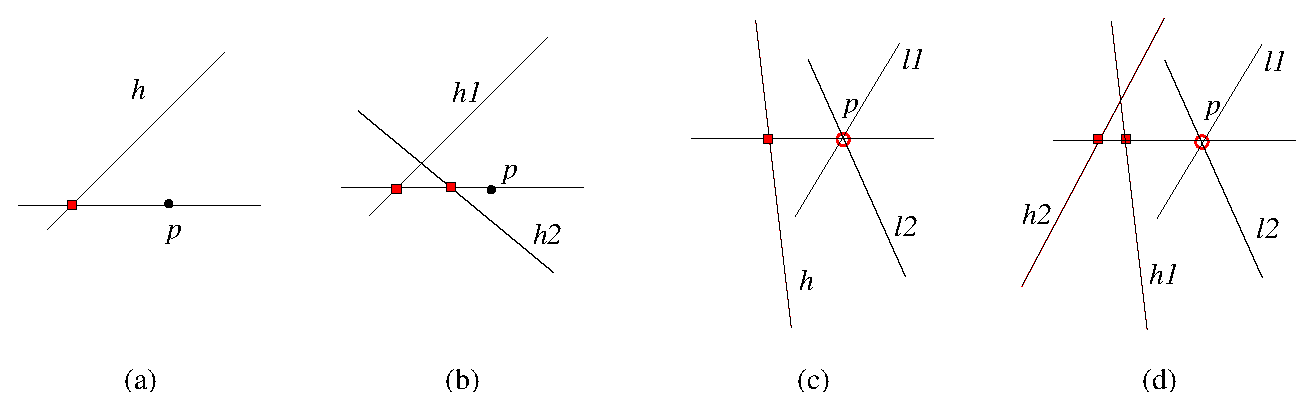
\includegraphics[width=\textwidth]{Kernel_23_ref/fig/compare_x_at_y}}
\caption{Comparison of the $x$-coordinates of the (implicitly given)
         points in the boxes, at a $y$-coordinate. The $y$-coordinate
         is either given explicitly (disc) or implicitly (circle).
         \label{fig-compare_x_at_y}}
\end{figure} 
\end{ccTexOnly} 

\ccFunction{Comparison_result compare_x_at_y(const Point_2<Kernel> &p,
                                             const Line_2<Kernel> &h1,
                                             const Line_2<Kernel> &h2);}
{This function compares the $x$-coordinates of the horizontal projection 
 of \ccStyle{p} on \ccStyle{h1} and on \ccStyle{h2}%
 \ccTexHtml{ (Figure~\ref{fig-compare_x_at_y} (b))}{; see (b) in the figure 
 below}.
\ccPrecond \ccStyle{h1} and \ccStyle{h2} are not horizontal.
}

\ccFunction{Comparison_result compare_x_at_y(const Line_2<Kernel> &l1,
                                           const Line_2<Kernel> &l2,
                                           const Line_2<Kernel> &h);}
      {Let $p$ be the \ccHtmlNoLinksFrom{intersection} of lines $l1$ and $l2$.
       This function compares the $x$-coordinates of $p$ and 
       the horizontal projection of \ccStyle{p} on \ccStyle{h}%
       \ccTexHtml{ (Figure~\ref{fig-compare_x_at_y} (c))}{; see (c) in the 
       figure below}.
       \ccPrecond \ccStyle{l1} and \ccStyle{l2} intersect and are not 
       horizontal; \ccStyle{h} is not horizontal.
}


\ccFunction{Comparison_result compare_x_at_y(const Line_2<Kernel> &l1,
                                             const Line_2<Kernel> &l2,
                                             const Line_2<Kernel> &h1,
                                             const Line_2<Kernel> &h2);}
{Let $p$ be the \ccHtmlNoLinksFrom{intersection} of lines $l1$ and $l2$. This 
 function compares the $x$-coordinates of the horizontal projection of 
 \ccStyle{p} on \ccStyle{h1} and on \ccStyle{h2}%
 \ccTexHtml{ (Figure~\ref{fig-compare_x_at_y} (d))}{; see (d) in the figure 
 below}.
\ccPrecond \ccStyle{l1} and \ccStyle{l2} intersect and are not horizontal; 
 \ccStyle{h1} and \ccStyle{h2} are not horizontal.
}

\begin{ccHtmlOnly}
<img border=0 src="fig/compare_x_at_y.gif" align=middle alt="Comparison of x at y"> 
\end{ccHtmlOnly} 

\ccSeeAlso
\ccRefIdfierPage{CGAL::compare_xy} \\
\ccRefIdfierPage{CGAL::compare_xyz} \\
\ccRefIdfierPage{CGAL::compare_x} \\
\ccRefIdfierPage{CGAL::compare_y} \\
\ccRefIdfierPage{CGAL::compare_yx} \\
\ccRefIdfierPage{CGAL::compare_y_at_x} \\
\ccRefIdfierPage{CGAL::compare_z} \\

\end{ccRefFunction}


\KernelRefLayout
\begin{ccRefFunction}{compare_y}

\ccFunction{Comparison_result compare_y(const Point_2<Kernel> &p,
                            	        const Point_2<Kernel> &q);}
	{compares Cartesian $y$-coordinates of $p$ and $q$.}

\ccFunction{Comparison_result compare_y(const Point_3<Kernel> &p,
                            	        const Point_3<Kernel> &q);}
	{compares Cartesian $y$-coordinates of $p$ and $q$.}

\begin{ccHtmlOnly}
<img border=0 src=./compare1.gif align=center alt="Comparison of the x 
or y coordinates of the (implicitly given) points in the boxes">
\end{ccHtmlOnly} 

\begin{ccTexOnly}
\begin{figure}[hb]
\centerline{\Ipe{compare1.ipe}}
\caption{Comparison of the $x$ or $y$-coordinates of the (implicitly
given) points in the boxes.\label{fig-compare13}}
\end{figure} 
\end{ccTexOnly} 

\ccFunction{Comparison_result compare_y(const Point_2<Kernel> &p,
                                        const Line_2<Kernel> &l1,
                                        const Line_2<Kernel> &l2);}
        {compares the $y$-coordinates of $p$ and the \ccHtmlNoLinksFrom{intersection} of lines
         $l1$ and $l2$%
         \ccTexHtml{ (Figure~\ref{fig-compare13} (a))}{, see (a) in the figure 
         above}.}


\ccFunction{Comparison_result compare_y(const Line_2<Kernel> &l,
                                        const Line_2<Kernel> &h1,
                                        const Line_2<Kernel> &h2);}
        {compares the $y$-coordinates of the \ccHtmlNoLinksFrom{intersection} of line $l$
         with line $h1$ and with line $h2$%
         \ccTexHtml{ (Figure~\ref{fig-compare13} (b))}{, see (b) in the figure 
         above}.}


\ccFunction{Comparison_result compare_y(const Line_2<Kernel> &l1,
                                        const Line_2<Kernel> &l2,
                                        const Line_2<Kernel> &h1,
                                        const Line_2<Kernel> &h2);}
        {compares the $y$-coordinates of the \ccHtmlNoLinksFrom{intersection} of lines $l1$
         and $l2$ and  the \ccHtmlNoLinksFrom{intersection} of lines $h1$ and $h2$ 
         \ccTexHtml{ (Figure~\ref{fig-compare13} (c))}{, see (c) in the figure 
         above}.}

\ccSeeAlso
\ccRefIdfierPage{CGAL::compare_xy} \\
\ccRefIdfierPage{CGAL::compare_xyz} \\
\ccRefIdfierPage{CGAL::compare_x} \\
\ccRefIdfierPage{CGAL::compare_x_at_y} \\
\ccRefIdfierPage{CGAL::compare_yx} \\
\ccRefIdfierPage{CGAL::compare_y_at_x} \\
\ccRefIdfierPage{CGAL::compare_z} \\

\end{ccRefFunction}


\KernelRefLayout
\begin{ccRefFunction}{compare_y_at_x}

Depending on which \cgal\ \ccHtmlNoLinksFrom{kernel} is used,
different versions of this global function are available. This is
described below.

%%%%%%%%%%%%%%%%%%%%%%%%%%%%%%%%%%%%%%%%%%%%%%
\paragraph{With the basic 2D and 3D Kernel} (see Chapter~\ref{chapter-kernel-23})

\ccFunction{Comparison_result compare_y_at_x(const Point_2<Kernel> &p,
                                             const Line_2<Kernel> &h);}
        {compares the $y$-coordinates of $p$ and the vertical projection
         of \ccStyle{p} on \ccStyle{h}%
         \ccTexHtml{ (Figure~\ref{fig-compare2} (d))}{, see (d) in the figure 
         below}.
         \ccPrecond \ccStyle{h} is not vertical.
         }

 \begin{ccTexOnly}
\begin{figure}[h]
\centerline{\includegraphics{Kernel_23_ref/fig/compare2}}
\caption{Comparison of the $y$-coordinates of the (implicitly given)
         points in the boxes, at an $x$-coordinate. The $x$-coordinate
         is either given explicitly (disc) or implicitly (circle).
         \label{fig-compare2}}
\end{figure} 
\end{ccTexOnly} 

\ccFunction{Comparison_result compare_y_at_x(const Point_2<Kernel> &p,
                                           const Line_2<Kernel> &h1,
                                           const Line_2<Kernel> &h2);}
{compares the $y$-coordinates of the vertical projection 
 of \ccStyle{p} on \ccStyle{h1} and on \ccStyle{h2}%
 \ccTexHtml{ (Figure~\ref{fig-compare2} (e))}{, see (e) in the figure 
 below}.
\ccPrecond \ccStyle{h1} and \ccStyle{h2} are not vertical.
}


\ccFunction{Comparison_result compare_y_at_x(const Line_2<Kernel> &l1,
                                           const Line_2<Kernel> &l2,
                                           const Line_2<Kernel> &h);}
      {Let $p$ be the \ccHtmlNoLinksFrom{intersection} of lines $l1$ and $l2$.
       This function compares the $y$-coordinates of $p$ and 
       the vertical projection of \ccStyle{p} on \ccStyle{h}%
       \ccTexHtml{ (Figure~\ref{fig-compare2} (f))}{, see (f) in the figure 
       below}.
       \ccPrecond \ccStyle{l1}, \ccStyle{l2} intersect and \ccStyle{h} is not
       vertical.
      }


\ccFunction{Comparison_result compare_y_at_x(const Line_2<Kernel> &l1,
                                           const Line_2<Kernel> &l2,
                                           const Line_2<Kernel> &h1,
                                           const Line_2<Kernel> &h2);}
{Let $p$ be the \ccHtmlNoLinksFrom{intersection} of lines $l1$ and $l2$. This function 
 compares the $y$-coordinates of the vertical projection of \ccStyle{p} on 
 \ccStyle{h1} and on \ccStyle{h2}%
 \ccTexHtml{ (Figure~\ref{fig-compare2} (g))}{, see (g) in the figure 
 below}.
 \ccPrecond \ccStyle{l1} and \ccStyle{l2} intersect; \ccStyle{h1} and 
 \ccStyle{h2} are not vertical.
}

\ccFunction{Comparison_result compare_y_at_x(const Point_2<Kernel> &p,
                                             const Segment_2<Kernel> &s);}
{compares the $y$-coordinates of $p$ and the vertical projection
 of \ccStyle{p} on \ccStyle{s}.  If \ccc{s} is vertical, then return
 \ccc{EQUAL} when \ccc{p} lies on \ccc{s}, \ccc{SMALLER} when \ccc{p} lies
 under {s}, and \ccc{LARGER} otherwise.
 \ccPrecond \ccStyle{p} is within the x range of \ccStyle{s}.}

\ccFunction{Comparison_result compare_y_at_x(const Point_2<Kernel> &p,
                                           const Segment_2<Kernel> &s1,
                                           const Segment_2<Kernel> &s2);}
{compares the $y$-coordinates of the vertical projection 
 of \ccStyle{p} on \ccStyle{s1} and on \ccStyle{s2}.  If \ccc{s1} or \ccc{s2}
 is vertical, then return \ccc{EQUAL} if they intersect, otherwise return
 \ccc{SMALLER} if \ccc{s1} lies below \ccc{s2}, and return \ccc{LARGER}
 otherwise.
 \ccPrecond \ccStyle{p} is within the x range of \ccStyle{s1} and \ccStyle{s2}.}


\begin{ccHtmlOnly}
<img border=0 src="fig/compare2.gif" align=middle alt="Comparison of y at x">
\end{ccHtmlOnly} 

%%%%%%%%%%%%%%%%%%%%%%%%%%%%%%%%%%%%%%%%%%%%%%
\paragraph{With the 2D Circular Kernel} (see Chapter~\ref{chapter-circular-kernel}) 

\ccInclude{CGAL/global_functions_circular_kernel_2.h}

If this kernel is used, in addition to the function and the
combination of 2D types described above, another version of the function
is provided.

\ccFunction{Comparison_result 
  compare_y_at_x(const Circular_arc_point_2<CircularKernel> &p, 
                 const Circular_arc_2<CircularKernel> &a);}
{Same as above, for a point and a circular arc.}

\ccFunction{Comparison_result 
  compare_y_at_x(const Circular_arc_point_2<CircularKernel> &p, 
                 const Line_arc_2<CircularKernel> &a);}
{Same as above, for a point and a line segment.}

\ccSeeAlso
\ccRefIdfierPage{CGAL::compare_xy} \\
\ccRefIdfierPage{CGAL::compare_xyz} \\
\ccRefIdfierPage{CGAL::compare_x} \\
\ccRefIdfierPage{CGAL::compare_x_at_y} \\
\ccRefIdfierPage{CGAL::compare_y} \\
\ccRefIdfierPage{CGAL::compare_yx} \\
\ccRefIdfierPage{CGAL::compare_z} \\

\end{ccRefFunction}


\KernelRefLayout
\begin{ccRefFunction}{compare_z}

\ccFunction{Comparison_result compare_z(const Point_3<R> &p,
                            	        const Point_3<R> &q);}
        {compares the $z$-coordinates of $p$ and $q$.}

\end{ccRefFunction}


\KernelRefLayout
\begin{ccRefEnum}{Comparison_result}
\ccInclude{CGAL/enum.h}

\ccGlobalEnum{enum  Comparison_result { SMALLER, EQUAL, LARGER };}

\ccRefLabel{SMALLER}
\ccRefLabel{EQUAL}
\ccRefLabel{LARGER}
\ccHtmlCrossLink{SMALLER}
\ccHtmlCrossLink{EQUAL}
\ccHtmlCrossLink{LARGER}

\end{ccRefEnum}


\KernelRefLayout
\begin{ccRefConstant}{COPLANAR}
\ccGlobalVariable{const Orientation COPLANAR  = ZERO;}

\ccSeeAlso
\ccc{NEGATIVE},
\ccc{POSITIVE}
\end{ccRefConstant}

\KernelRefLayout
\begin{ccRefFunction}{coplanar}

\ccFunction{bool coplanar(const Point_3<Kernel> &p,
                               const Point_3<Kernel>&q,
                               const Point_3<Kernel>&r,
                               const Point_3<Kernel>&s);}
{returns \ccStyle{true}, if $p$, $q$, $r$, and $s$ are coplanar.}

\ccSeeAlso
\ccRefIdfierPage{CGAL::coplanar_orientation} \\
\ccRefIdfierPage{CGAL::coplanar_side_of_bounded_circle} \\

\end{ccRefFunction}


\KernelRefLayout
\begin{ccRefFunction}{coplanar_orientation}

\ccFunction{Orientation coplanar_orientation(const Point_3<R>& p,
                                 const Point_3<R>& q,
                                 const Point_3<R>& r,
                                 const Point_3<R>& s);}
         {Let $P$ be the plane defined by the points \ccc{p}, \ccc{q},
          and \ccc{r}. Note that the order defines the orientation of
          $P$. The function computes the orientation of points \ccc{p}, 
          \ccc{q}, and \ccc{s} in $P$: Iff \ccc{p}, \ccc{q}, \ccc{s} are
          collinear, \ccc{COLLINEAR} is returned. Iff $P$ and the plane 
          defined by \ccc{p}, \ccc{q}, and \ccc{s} have the same orientation, 
          \ccc{POSITIVE} is returned; otherwise \ccc{NEGATIVE} is returned.  
          \ccPrecond \ccc{p}, \ccc{q}, \ccc{r}, and \ccc{s} are coplanar and
          \ccc{p}, \ccc{q}, and \ccc{r} are not collinear.}
\end{ccRefFunction}


\KernelRefLayout
\begin{ccRefFunction}{coplanar_side_of_bounded_circle}

\ccFunction{Bounded_side coplanar_side_of_bounded_circle(const Point_3<R>& p,
                                 const Point_3<R>& q,
                                 const Point_3<R>& r,
                                 const Point_3<R>& s);}
         {returns the bounded side of the circle defined
          by \ccc{p}, \ccc{q}, and \ccc{r} on which \ccc{s} lies.
          \ccPrecond \ccc{p}, \ccc{q}, \ccc{r}, and \ccc{s} are coplanar and
          \ccc{p}, \ccc{q}, and \ccc{r} are not collinear.}

\ccSeeAlso
\ccRefIdfierPage{CGAL::coplanar_orientation} \\
\ccRefIdfierPage{CGAL::side_of_bounded_circle} \\

\end{ccRefFunction}


\KernelRefLayout
\begin{ccRefConstant}{COUNTERCLOCKWISE}
\ccGlobalVariable{const Orientation COUNTERCLOCKWISE = POSITIVE;}
\end{ccRefConstant}

\KernelRefLayout
\begin{ccRefFunction}{cross_product}

\ccFunction{Vector_3<R> cross_product( const Vector_3<R>& u, 
                                       const Vector_3<R>& v);}
       {returns the cross product of $u$ and $v$.}
\end{ccRefFunction}


\KernelRefLayout
\begin{ccRefConstant}{DEGENERATE}
\ccGlobalVariable{const Orientation DEGENERATE = ZERO;}
\end{ccRefConstant}

\KernelRefLayout
\begin{ccRefClass} {Direction_2<R>}

\ccDefinition
An object of the class \ccRefName\ is a vector in the two-dimensional 
vector space $\R^2$  where we forget about its length. They can be
viewed as unit vectors, although there is no normalization internally,
since this is error prone.  Directions are used whenever the length of
a vector does not matter. 
They also characterize a set of parallel oriented lines that have the same
orientations.  
For example, you can ask for the direction
orthogonal to an oriented plane, or the direction of an oriented line.
Further, they can be used to indicate angles. The slope of a direction
is \ccStyle{dy()/dx()}.


\ccCreation
\ccCreationVariable{d}


\ccHidden \ccConstructor{Direction_2();}
             {introduces an uninitialized direction \ccVar.}

\ccHidden \ccConstructor{Direction_2(const Direction_2<R> &d);}
            {copy constructor.}

\ccConstructor{Direction_2(const Vector_2<R> &v);}
            {introduces the direction \ccVar\ of vector $v$.}

\ccConstructor{Direction_2(const Line_2<R> &l);}
            {introduces the direction \ccVar\ of line $l$.}

\ccConstructor{Direction_2(const Ray_2<R> &r);}
            {introduces the direction \ccVar\ of ray $r$.}

\ccConstructor{Direction_2(const Segment_2<R> &s);}
            {introduces the direction \ccVar\ of segment $s$.}

\ccConstructor{Direction_2(const R::RT &x, const R::RT &y);}
            {introduces a direction \ccVar\ passing through the origin
             and the point with Cartesian coordinates $(x, y)$.}


\ccOperations
%\ccSetTwoOfThreeColumns{5cm}{4cm}
\ccSetThreeColumns{Direction_2<R> & }{}{\hspace*{7.8cm}}

\ccHidden \ccMethod{Direction_2<R> & operator=(const Direction_2<R> &e);}
        {Assignment.}

\ccMethod{R::RT delta(int i) const;}
       {returns values, such that \ccVar \ccc{== Direction_2<R>(delta(0),delta(1))}.
        \ccPrecond: $0 \leq i \leq 1$.}

\ccMethod{R::RT dx() const;}
       {returns \ccc{delta(0)}.}

\ccMethod{R::RT dy() const;}
       {returns \ccc{delta(1)}.}

There is a total order on directions. We compare the angles between the
positive $x$-axis and the directions in counterclockwise order.

\ccMethod{bool operator==(const Direction_2<R> &e) const;}
       {}
\ccGlue
\ccMethod{bool operator!=(const Direction_2<R> &e) const;}
       {}
\ccGlue
\ccMethod{bool operator<(const Direction_2<R> &e) const;}
       {}
\ccGlue
\ccMethod{bool operator>(const Direction_2<R> &e) const;}
       {}
\ccGlue
\ccMethod{bool operator<=(const Direction_2<R> &e) const;}
       {}
\ccGlue
\ccMethod{bool operator>=(const Direction_2<R> &e) const;}
       {}

Furthermore, we have

\ccMethod{bool counterclockwise_in_between(const Direction_2<R> &d1,
                                   const Direction_2<R> &d2) const;}
       {returns true, iff \ccVar\ is not equal to \ccc{d1}, and 
        while rotating counterclockwise starting at \ccc{d1}, 
        \ccVar\ is reached strictly before \ccc{d2} is reached.
        Note that true is returned if \ccc{d1} == \ccc{d2}, unless
        also \ccVar\ == \ccc{d1}.
       }


\ccMethod{Direction_2<R>  operator-() const;}
       {The direction opposite to \ccVar.}

\ccHeading{Miscellaneous}

\ccMethod{Vector_2<R> vector() const;}
       {returns a vector that has the same direction as \ccVar.}

\ccMethod{Direction_2<R>  transform(const Aff_transformation_2<R> &t) const;}
       {returns the direction obtained by applying $t$ on \ccVar.}

\ccSeeAlso
\ccRefConceptPage{Kernel::Direction_2} \\

\end{ccRefClass} 

 
\KernelRefLayout
\begin{ccRefClass}{Direction_3<R>}

\ccDefinition
An object of the class \ccRefName\ is a vector in the three-dimensional 
vector space $\R^3$  where we forget about their length. They can be
viewed as unit vectors, although there is no normalization internally,
since this is error prone.  Directions are used whenever the length of
a vector does not matter. 
They also characterize a set of parallel lines that have the same orientation 
or the direction normal to parallel planes that have the same orientation.
For example, you can ask for the direction
orthogonal to an oriented plane, or the direction of an oriented line.


\ccCreation
\ccCreationVariable{d}


\ccHidden \ccConstructor{Direction_3();}
             {introduces an uninitialized direction \ccVar.}

\ccHidden \ccConstructor{Direction_3(const Direction_3<R> &d);}
            {copy constructor.}

\ccConstructor{Direction_3(const Vector_3<R> &v);}
            {introduces a direction \ccVar\ initialised with the 
             direction of vector $v$.}

\ccConstructor{Direction_3(const Line_3<R> &l);}
            {introduces the direction \ccVar\ of line $l$.}

\ccConstructor{Direction_3(const Ray_3<R> &r);}
            {introduces the direction \ccVar\ of ray $r$.}

\ccConstructor{Direction_3(const Segment_3<R> &s);}
            {introduces the direction \ccVar\ of segment $s$.}

\ccConstructor{Direction_3(const R::RT &x, const R::RT &y, const R::RT &z);}
            {introduces a direction \ccVar\ initialised with the direction 
             from the origin to the point with Cartesian coordinates $(x, y, z)$.}


\ccOperations
%\ccSetTwoOfThreeColumns{5cm}{4cm}
\ccSetThreeColumns{Direction_3<R> & }{}{\hspace*{7.8cm}}

\ccHidden \ccMethod{Direction_3<R> & operator=(const Direction_3<R> &e);}
        {Assignment.}

\ccMethod{R::RT delta(int i) const;}
       {returns values, such that \ccVar \ccc{== Direction_3<R>(delta(0),delta(1),delta(2))}.
        \ccPrecond: $0 \leq i \leq 2$.}

\ccMethod{R::RT dx() const;}
       {returns \ccc{delta(0)}.}
\ccGlue
\ccMethod{R::RT dy() const;}
       {returns \ccc{delta(1)}.}
\ccGlue
\ccMethod{R::RT dz() const;}
       {returns \ccc{delta(2)}.}


\ccMethod{bool operator==(const Direction_3<R> &e) const;}
       {Test for equality.}
\ccGlue
\ccMethod{bool operator!=(const Direction_3<R> &e) const;}
       {Test for inequality.}


\ccMethod{Direction_3<R>  operator-() const;}
       {The direction opposite to \ccVar.}

\ccMethod{Vector_3<R> vector() const;}
       {returns a vector that has the same direction as \ccVar.}

\ccMethod{Direction_3<R>  transform(const Aff_transformation_3<R> &t) const;}
       {returns the direction obtained by applying $t$ on \ccVar.}

\ccSeeAlso
\ccRefConceptPage{Kernel::Direction_3}

\end{ccRefClass} 


\KernelRefLayout
\begin{ccRefFunction}{do_intersect}
\ccInclude{CGAL/intersections.h}

\ccUnchecked{
\ccFunction{bool do_intersect(Type1<Kernel> obj1, Type2<Kernel> obj2);}
{checks whether \ccc{obj1} and \ccc{obj2} intersect.
Two objects \ccStyle{obj1} and \ccStyle{obj2} intersect if there is a point
\ccStyle{p} that is part of both \ccStyle{obj1} and \ccStyle{obj2}.
The \ccHtmlNoLinksFrom{intersection} region of those two objects is defined as the set of all
points \ccStyle{p} that are part of both \ccStyle{obj1} and \ccStyle{obj2}.
Note that for objects like triangles and polygons that enclose a
bounded region, this region is part of the object.
}}

The types \ccStyle{Type1} and \ccStyle{Type2} can be any of the following:
\begin{itemize}\ccTexHtml{\itemsep0pt\topsep0pt\partopsep0pt\parskip0pt\parsep0pt}{}
\item \ccStyle{Point_2<Kernel>}
\item \ccStyle{Line_2<Kernel>}
\item \ccStyle{Ray_2<Kernel>}
\item \ccStyle{Segment_2<Kernel>}
\item \ccStyle{Triangle_2<Kernel>}
\item \ccStyle{Iso_rectangle_2<Kernel>}
\end{itemize}

Also, in three-dimensional space \ccc{Type1} can be \ccc{Plane_3<Kernel>} or
\ccc{Triangle_3<Kernel>} and \ccc{Type2} any of 
\begin{itemize}\ccTexHtml{\itemsep0pt\topsep0pt\partopsep0pt\parskip0pt\parsep0pt}{}
\item \ccStyle{Plane_3<Kernel>}
\item \ccStyle{Line_3<Kernel>}
\item \ccStyle{Ray_3<Kernel>}
\item \ccStyle{Segment_3<Kernel>}
\item \ccStyle{Triangle_3<Kernel>}
\end{itemize}
Finally, \ccc{Type1} can be of type \ccc{Triangle_3<Kernel>} and \ccc{Type2} of type \ccc{Tetrahedron_3<Kernel>}.

\ccSeeAlso
\ccRefIdfierPage{CGAL::intersection}

\end{ccRefFunction}

\KernelRefLayout
\begin{ccRefFunction}{do_overlap}
\ccInclude{CGAL/Bbox_2.h}

\ccFunction{bool do_overlap(const Bbox_2 &bb1, const Bbox_2 &bb2);}
       {returns \ccc{true} iff \ccc{bb1} and \ccc{bb2} overlap, i.e.,
        iff their \ccHtmlNoLinksFrom{intersection} is non-empty.}

\ccInclude{CGAL/Bbox_3.h}

\ccFunction{bool do_overlap(const Bbox_3 &bb1, const Bbox_3 &bb2);}
       {returns \ccc{true} iff \ccc{bb1} and \ccc{bb2} overlap, i.e.,
        iff their \ccHtmlNoLinksFrom{intersection} is non-empty.}
\end{ccRefFunction}


\KernelRefLayout
\begin{ccRefConcept}{FieldNumberType}

The concept \ccRefName\ defines the syntactic requirements of a number type
to be used as a template parameter for the Cartesian kernels.  This number
type supports the operations $+$, $-$, $*$ and $/$.  This implies that
\ccc{CGAL::Number_type_traits<FieldNumberType>::Has_division} is
\ccc{CGAL::Tag_true}.

\ccRefines
RingNumberType

\ccHasModels
\ccc{float} \\
\ccc{double} \\
\ccc{CGAL::Filtered_exact<FieldNumberType, ET>} \\
\ccc{CGAL::Fixed_precision_nt} \\
\ccc{CGAL::Gmpq} \\
\ccc{CGAL::Interval_nt} \\
\ccc{CGAL::Interval_nt_advanced} \\
\ccc{CGAL::Lazy_exact_nt<FieldNumberType>} \\
\ccc{CGAL::MP_Float} \\
\ccc{CGAL::Quotient<RingNumberType>} \\
\ccc{leda_rational} \\
\ccc{leda_bigfloat} \\
\ccc{leda_real} \\

\ccCreationVariable{ntvar}

\ccOperations
\ccFunction{FieldNumberType operator/(const FieldNumberType &ntval1, 
                                      const FieldNumberType &ntval2);}
       {}

\ccMethod{FieldNumberType operator/=(const FieldNumberType &n) const;}{}


\ccSeeAlso
\ccRefConceptPage{EuclideanRingNumberType} \\
\ccRefConceptPage{Kernel} \\
\ccRefIdfierPage{Field_tag} \\
Support Library Manual

\end{ccRefConcept}

\KernelRefLayout
\input{Ref/has_larger_dist_to_point.tex}
\KernelRefLayout
\begin{ccRefFunction}{has_larger_signed_dist_to_line}

\ccFunction{bool
has_larger_signed_dist_to_line(const Line_2<R>&  l,
                               const Point_2<R>& p,
                               const Point_2<R>& q);}
          {returns \ccStyle{true} iff the signed distance of \ccStyle{p}
           and \ccStyle{l} is larger than the signed distance of 
           \ccStyle{q} and \ccStyle{l}.}

\ccFunction{bool
has_larger_signed_dist_to_line(const Point_2<R>& p,
                               const Point_2<R>& q,
                               const Point_2<R>& r,
                               const Point_2<R>& s);}
          {returns \ccStyle{true} iff the signed distance of \ccStyle{r}
           and \ccStyle{l} is larger than the signed distance of 
           \ccStyle{s} and \ccStyle{l}, where \ccc{l} is the directed line
           through points \ccc{p} and \ccc{q}.}


\end{ccRefFunction}


\KernelRefLayout
\input{Ref/has_larger_signed_dist_to_plane.tex}
\KernelRefLayout
\begin{ccRefFunction}{has_smaller_dist_to_point}
\ccInclude{CGAL/distance_predicates_2.h}

\ccFunction{bool
has_smaller_dist_to_point(const Point_2<R>& p,
                          const Point_2<R>& q,
                          const Point_2<R>& r);}
         {returns \ccStyle{true} iff the distance between \ccStyle{q}
          and \ccStyle{p} is smaller than the distance between \ccStyle{r}
          and \ccStyle{p}.}

\ccInclude{CGAL/distance_predicates_3.h}

\ccFunction{bool
has_smaller_dist_to_point(const Point_3<R>& p,
                          const Point_3<R>& q,
                          const Point_3<R>& r);}
         {returns \ccStyle{true} iff the distance between \ccStyle{q}
          and \ccStyle{p} is smaller than the distance between \ccStyle{r}
          and \ccStyle{p}.}
\end{ccRefFunction}


\KernelRefLayout
\begin{ccRefFunction}{has_smaller_signed_dist_to_line}

\ccFunction{bool
has_smaller_signed_dist_to_line(const Line_2<R>&  l,
                                const Point_2<R>& p,
                                const Point_2<R>& q);}
          {returns \ccStyle{true} iff the signed distance of \ccStyle{p}
           and \ccStyle{l} is smaller than the signed distance of 
           \ccStyle{q} and \ccStyle{l}.}

\ccFunction{bool
has_smaller_signed_dist_to_line(const Point_2<R>& p,
                                const Point_2<R>& q,
                                const Point_2<R>& r,
                                const Point_2<R>& s);}
          {returns \ccStyle{true} iff the signed distance of \ccStyle{r}
           and \ccStyle{l} is smaller than the signed distance of 
           \ccStyle{s} and \ccStyle{l}, where \ccc{l} is the 
           oriented line through \ccc{p} and \ccc{q}.}
\end{ccRefFunction}


\KernelRefLayout
\begin{ccRefFunction}{has_smaller_signed_dist_to_plane}

\ccFunction{bool
has_smaller_signed_dist_to_plane(const Plane_3<R>& h,
                                 const Point_3<R>& p,
                                 const Point_3<R>& q);}
          {returns \ccStyle{true} iff the signed distance of \ccStyle{p}
           and \ccStyle{h} is smaller than the signed distance of 
           \ccStyle{q} and \ccStyle{h}.}

\ccFunction{bool
has_smaller_signed_dist_to_plane(const Point_3<R>& p,
                                 const Point_3<R>& q,
                                 const Point_3<R>& r,
                                 const Point_3<R>& s,
                                 const Point_3<R>& t);}
          {returns \ccStyle{true} iff the signed distance of \ccStyle{p}
           and \ccStyle{h} is smaller than the signed distance of 
           \ccStyle{q} and \ccStyle{h}, where \ccc{h} is the oriented
           plane through \ccc{p}, \ccc{q} and \ccc{r}.}
\end{ccRefFunction}


\KernelRefLayout
\begin{ccRefClass}{Homogeneous<RingNumberType>}
\ccInclude{CGAL/Homogeneous.h}

\ccDefinition
A model for a \ccc{Kernel} using homogeneous coordinates to represent the
geometric objects.  In order for \ccRefName\ to model Euclidean geometry
in $E^2$ and/or $E^3$, for some mathematical ring $E$ (\textit{e.g.},
the integers \Z\ or the rationals \Q), the template parameter \ccc{RingNumberType}
must model the mathematical ring $E$.  That is, the ring operations on this
number type must compute the mathematically correct results.  If the number
type provided as a model for \ccc{RingNumberType} is only an approximation of a
ring (such as the built-in type \ccc{double}), then the geometry provided by
the kernel is only an approximation of Euclidean geometry.  

\ccIsModel
\ccRefConceptPage{Kernel}

\ccTexHtml{\ccSetThreeColumns{typedef Quotient<RingNumberType>}{}{\hspace*{8.5cm}}}{}
\ccTypes
\ccTypedef{typedef Quotient<RingNumberType> FT;}{}
\ccGlue
\ccTypedef{typedef RingNumberType RT;}{}

\ccImplementation
This model of a kernel uses reference counting.

\ccSeeAlso
\ccRefIdfierPage{CGAL::Cartesian<FieldNumberType>} \\
\ccRefIdfierPage{CGAL::Simple_cartesian<FieldNumberType>} \\
\ccRefIdfierPage{CGAL::Simple_homogeneous<RingNumberType>} \\

\end{ccRefClass}

\KernelRefLayout
\begin{ccRefClass}{Homogeneous_converter<K1, K2,
                             RT_Converter = NT_converter<K1::RT, K2::RT>,
                             FT_Converter = NT_converter<K1::FT, K2::FT> >}
%\ccTexHtml{\ccSetThreeColumns{Point_2< us<RT> > }{}{\hspace*{8.5cm}}}{}

\KernelRefLayout\gdef\ccTagOperatorLayout{\ccFalse}

\ccDefinition

\ccClassTemplateName converts objects from the kernel traits \ccc{K1} to
the kernel traits \ccc{K2}.  Those traits must be of the form
\ccc{Homogeneous<RT1>} and \ccc{Homogeneous<RT2>} (or the equivalent with
\ccc{Simple_homogeneous}).  It then provides the following operators to
convert objects from \ccc{K1} to \ccc{K2}.

\ccInclude{CGAL/Homogeneous_converter.h}

\ccTypes

The third template parameter \ccc{RT_Converter} is a function object that must
satisfy:

\ccMemberFunction{K2::RT operator()(const K1::RT &n);}
{ converts \ccc{n} to an \ccc{K2::RT} which has the same value.}

The default value of this parameter uses the conversion operator from
\ccc{K1::RT} to \ccc{K2::RT}.

Similarly for the fourth template parameter which must satisfy:

\ccMemberFunction{K2::FT operator()(const K1::FT &n);}
{ converts \ccc{n} to an \ccc{K2::FT} which has the same value.}

\ccCreation
\ccCreationVariable{conv}

\ccConstructor{Homogeneous_converter<>();}{Default constructor.}

\ccOperations

\ccMemberFunction{K2::Point_2 operator()(const K1::Point_2&p);}
{ returns a \ccc{K2::Point_2} which coordinates are those of \ccc{p},
converted by \ccc{RT_Converter}.}

Similar operators are defined for the other kernel traits types \ccc{Point_3},
\ccc{Vector_2}...


%\ccTexHtml{\KernelRefLayout}{}
\end{ccRefClass}


\KernelRefLayout
\begin{ccRefFunction}{homogeneous_to_cartesian}
\ccTexHtml{\ccSetThreeColumns{Point_2< Homogeneous<RT> > }{}{\hspace*{8.5cm}}}{}

\ccInclude{CGAL/cartesian_homogeneous_conversion.h}

\ccFunction{Point_2< Cartesian<FT> >
homogeneous_to_cartesian(const Point_2< Homogeneous<FT> >& hp);}
        {converts 2d point \ccStyle{hp} with homogeneous representation  
         into a 2d point with Cartesian representation with the same
         number type.}

\ccFunction{Point_3< Cartesian<FT> >
homogeneous_to_cartesian(const Point_3< Homogeneous<FT> >& hp);}
        {converts 3d point \ccStyle{hp} with homogeneous representation  
         into a 3d point with Cartesian representation with the same
         number type.}
\end{ccRefFunction}


\KernelRefLayout
\begin{ccRefFunction}{homogeneous_to_quotient_cartesian}

\ccInclude{CGAL/cartesian_homogeneous_conversion.h}

\ccFunction{Point_2< Cartesian<Quotient<RT> > >
homogeneous_to_quotient_cartesian(
  const Point_2<Homogeneous<RT> >& hp);}
        {converts the 2d point \ccStyle{hp} with homogeneous representation  
         with number type \ccStyle{RT} into a 2d point with Cartesian 
         representation with number type \ccStyle{Quotient<RT>}.}

\ccFunction{Point_3< Cartesian<Quotient<RT> > >
homogeneous_to_quotient_cartesian(
  const Point_3<Homogeneous<RT> >& hp);}
        {converts the 3d point \ccStyle{hp} with homogeneous representation  
         with number type \ccStyle{RT} into a 3d point with Cartesian 
         representation with number type \ccStyle{Quotient<RT>}.}

\ccSeeAlso

\ccRefIdfierPage{CGAL::Cartesian<FieldNumberType>} \\
\ccRefIdfierPage{CGAL::Cartesian_converter<K1, K2, NTConverter>} \\
\ccRefIdfierPage{CGAL::cartesian_to_homogeneous} \\
\ccRefIdfierPage{CGAL::Homogeneous<RingNumberType>} \\
\ccRefIdfierPage{CGAL::Homogeneous_converter<K1, K2, RTConverter, FTConverter>} \\
\ccRefIdfierPage{CGAL::homogeneous_to_cartesian} \\
\ccRefIdfierPage{CGAL::quotient_cartesian_to_homogeneous} \\
\ccRefIdfierPage{CGAL::Simple_cartesian<FieldNumberType>} \\
\ccRefIdfierPage{CGAL::Simple_homogeneous<RingNumberType>} \\


\end{ccRefFunction}


\KernelRefLayout
\begin{ccRefClass}{Identity_transformation}
\ccInclude{CGAL/aff_transformation_tags.h}

\ccDefinition
Tag class for affine transformations.

\ccSeeAlso
\ccRefIdfierPage{CGAL::Aff_transformation_2<R>} \\
\ccRefIdfierPage{CGAL::Aff_transformation_3<R>} \\
\ccRefIdfierPage{CGAL::Reflection} \\
\ccRefIdfierPage{CGAL::Rotation} \\
\ccRefIdfierPage{CGAL::Scaling} \\
\ccRefIdfierPage{CGAL::Translation} \\

\end{ccRefClass}

\KernelRefLayout
\begin{ccRefFunction}{intersection}
\ccInclude{CGAL/intersections_d.h}

\ccFunction{Kernel::Intersect_d::Result<Type1<K>, Type2<K> >::Type
  intersection(Type1<R> f1, Type2<R> f2);} { returns the intersection
  result of $f1$ and $f2$.
  \ccPrecond The objects are of the same dimension.}

The same functionality is also available through the functor \ccc{Kernel::Intersect_d}.

The possible value for types \ccStyle{Type1} and \ccStyle{Type2} and
the value for T\ldots in \ccStyle{boost::optional< boost::variant< T\ldots >} are the following:

\begin{ccTexOnly}
\begin{longtable}[c]{|l|l|l|}
%\caption{All available intersection computations}\\
\multicolumn{3}{l}{\sl \ \ }
\endfirsthead
\multicolumn{3}{l}{\sl continued}
\endhead
\hline
Type1 & Type2 & \parbox{4 cm}{\vspace{1 mm}{T\ldots}} \\
\hline
\ccStyle{Line_d} & \ccStyle{Line_d} & \parbox{4 cm}{\vspace{1 mm}
    \ccStyle{Point_d}, \ccStyle{Line_d}
  \vspace{1 mm}} \\
\hline
\ccStyle{Segment_d} & \ccStyle{Line_d} & \parbox{4 cm}{\vspace{1 mm}
    \ccStyle{Point_d}, \ccStyle{Segment_d}
  \vspace{1 mm}} \\
\hline
\ccStyle{Segment_d} & \ccStyle{Segment_d} & \parbox{4 cm}{\vspace{1 mm}
    \ccStyle{Point_d}, \ccStyle{Segment_d}
  \vspace{1 mm}} \\
\hline
\ccStyle{Ray_d} & \ccStyle{Line_d} & \parbox{4 cm}{\vspace{1 mm}
    \ccStyle{Point_d}, \ccStyle{Ray_d}
  \vspace{1 mm}} \\
\hline
\ccStyle{Ray_d} & \ccStyle{Segment_d} & \parbox{4 cm}{\vspace{1 mm}
    \ccStyle{Point_d}, \ccStyle{Segment_d}
  \vspace{1 mm}} \\
\hline
\ccStyle{Ray_d} & \ccStyle{Ray_d} & \parbox{4 cm}{\vspace{1 mm}
    \ccStyle{Point_d}, \ccStyle{Segment_d}, \ccStyle{Ray_d}
  \vspace{1 mm}} \\
\hline
\ccStyle{Hyperplane_d} & \ccStyle{Line_d} & \parbox{4 cm}{\vspace{1 mm}
\ccStyle{Point_3}, \ccStyle{Line_3} 
\vspace{1 mm}} \\
\hline
\ccStyle{Hyperplane_d} & \ccStyle{Ray_d} & \parbox{4 cm}{\vspace{1 mm}
\ccStyle{Point_d}, \ccStyle{Ray_d}
\vspace{1 mm}}  \\
\hline
\ccStyle{Hyperplane_d} & \ccStyle{Segment_d} & \parbox{4 cm}{\vspace{1 mm}
\ccStyle{Point_d}, \ccStyle{Segment_d}
\vspace{1 mm}}  \\
\hline
\end{longtable}
\end{ccTexOnly}

\begin{ccHtmlOnly}
<DIV ALIGN="CENTER">
<TABLE CELLPADDING=3 BORDER="1">
<TR> <TH> Type1 </TH>
 <TH> Type2 </TH>
 <TH> T... </TH>
</TR>
<TR>
    <TD VALIGN="CENTER" > Line_d </TD>
    <TD VALIGN="CENTER" > Line_d </TD>
    <TD><TABLE>
        <TR><TD>Point_d</TD></TR>
        <TR><TD>Line_d</TD></TR>
        </TABLE></TD>
</TR>
<TR>
    <TD VALIGN="CENTER" > Segment_d </TD>
    <TD VALIGN="CENTER" > Line_d </TD>
    <TD><TABLE>
        <TR><TD>Point_d</TD></TR>
        <TR><TD>Segment_d</TD></TR>
      </TABLE></TD>
</TR>
<TR>
    <TD VALIGN="CENTER" > Segment_d </TD>
    <TD VALIGN="CENTER" > Segment_d </TD>
    <TD><TABLE>
        <TR><TD>Point_d</TD></TR>
        <TR><TD>Segment_d</TD></TR>
      </TABLE></TD>
</TR>
<TR>
    <TD VALIGN="CENTER" > Ray_d </TD>
    <TD VALIGN="CENTER" > Line_d </TD>
    <TD><TABLE>
        <TR><TD>Point_d</TD></TR>
        <TR><TD>Ray_d</TD></TR>
      </TABLE></TD>
</TR>
<TR>
    <TD VALIGN="CENTER" > Ray_d </TD>
    <TD VALIGN="CENTER" > Segment_d </TD>
    <TD><TABLE>
        <TR><TD>Point_d</TD></TR>
        <TR><TD>Segment_d</TD></TR>
      </TABLE></TD>
</TR>
<TR>
    <TD VALIGN="CENTER" > Ray_d </TD>
    <TD VALIGN="CENTER" > Ray_d </TD>
    <TD><TABLE>
        <TR><TD>Point_d</TD></TR>
        <TR><TD>Segment_d</TD></TR>
        <TR><TD>Ray_d</TD></TR>
      </TABLE></TD>
</TR>
<TR>
    <TD VALIGN="CENTER" > Hyperplane_d </TD>
    <TD VALIGN="CENTER" > Line_d </TD>
    <TD><TABLE>
        <TR><TD>Point_d</TD></TR>
        <TR><TD>Line_d</TD></TR>
        </TABLE></TD>
</TR>
<TR>
    <TD VALIGN="CENTER" > Hyperplane_d </TD>
    <TD VALIGN="CENTER" > Ray_d </TD>
    <TD><TABLE>
        <TR><TD>Point_d</TD></TR>
        <TR><TD>Ray_d</TD></TR>
        </TABLE></TD>
</TR>
<TR>
    <TD VALIGN="CENTER" > Hyperplane_d </TD>
    <TD VALIGN="CENTER" > Segment_d </TD>
    <TD><TABLE>
        <TR><TD>Point_d</TD></TR>
        <TR><TD>Segment_d</TD></TR>
        </TABLE></TD>
</TR>
</TABLE>
</DIV>
\end{ccHtmlOnly}

\ccExample

The following example demonstrates the most common use of 
\ccc{intersection} routines.
\ccHtmlLinksOff%
\begin{verbatim}
#include <CGAL/intersections_d.h>

template<typename R>
struct Intersection_visitor {
  typedef result_type void;
  void operator()(const Point_d<R>& p) const { /* handle point */ }
  void operator()(const Segment_d<R>& s) const { /* handle segment */ }
};

template <class R>
void foo(Segment_d<R> seg, Line_d<R> lin)
{
  R::Intersect_d::template Result< Segment_d<R>, Line_d<R> > 
    result = intersection(seg, lin);
  if(result) { boost::apply_visitor(Intersection_visitor<R>(), *result); } 
  else { /* no intersection */ }
}
\end{verbatim}%
\ccHtmlLinksOn%

\ccSeeAlso 
\ccc{do_intersect}, \\
\ccc{Kernel::Intersect_d}, \\
\ccc{Kernel::Do_intersect_d}, \\ 
\ccAnchor{http://www.boost.org/doc/libs/release/libs/optional/index.html}{boost::optional}, \\
\ccAnchor{http://www.boost.org/doc/html/variant.html}{boost::variant} \\

\end{ccRefFunction}


\KernelRefLayout
\begin{ccRefClass} {Iso_cuboid_3<R>}
\ccInclude{CGAL/Iso_cuboid_3.h}

\ccDefinition  An object $s$ of the data type \ccRefName\ is a
cuboid in the Euclidean plane $\E^3$ with sides parallel to the $x$ and
$y$ axis of the coordinate system.
 
Although they are represented in a canonical form by only two
vertices, namely the lexicographically smallest and largest vertex
with respect to Cartesian $xyz$ coordinates, we provide
functions for ``accessing'' the other vertices as well.

Iso-oriented cuboids and bounding boxes are quite similar. The
difference however is that bounding boxes have always double coordinates, 
whereas the coordinate type of an iso-oriented cuboid is chosen by
the user.


\ccCreation
\ccCreationVariable{c}


\ccHidden \ccConstructor{Iso_cuboid_3();}
             {introduces an uninitialized variable \ccVar.}

\ccHidden \ccConstructor{Iso_cuboid_3(const Iso_cuboid_3<R> &u);}
 	    {copy constructor.}

\ccConstructor{Iso_cuboid_3(const Point_3<R> &p, 
	                    const Point_3<R> &q);}
            {introduces an iso-oriented cuboid \ccVar\ with diagonal
             opposite vertices $p$ and $q$. Note that the object is 
             brought in the canonical form.}


\ccOperations
\ccHidden \ccMethod{Iso_cuboid_3<R> & operator=(const Iso_cuboid_3<R> &q);}
        {Assignment.}

\ccMethod{bool operator==(const Iso_cuboid_3<R> &c2) const;}
       {Test for equality: two iso-oriented cuboid are equal, iff their
        lower left and their upper right vertices are equal.}

\ccMethod{bool operator!=(const Iso_cuboid_3<R> &c2) const;}
       {Test for inequality.}

\ccMethod{Point_3<R> vertex(int i) const;}
       {returns the i'th vertex modulo 8  of \ccVar.
        starting with the lower left vertex.}

\ccMethod{Point_3<R> operator[](int i) const;}
       {returns  \ccStyle{vertex(i)}, as indicated in the figure below:
       \lcTex{\epsfxsize=6cm\epsffile{IsoCuboid.eps}}}

\begin{ccHtmlOnly}
<center>
<img border=0 src=./IsoCuboid.gif align=center alt="vertex order of an iso-cuboid">
</center>
\end{ccHtmlOnly} 


\ccMethod{Point_3<R> min() const;}
       {returns the smallest vertex of \ccVar\ (= \ccStyle{vertex(0)}).}


\ccMethod{Point_3<R> max() const;}
       {returns the largest vertex of \ccVar\ (= \ccStyle{vertex(7)}).}
\ccMethod{ FT  xmin() const;}{returns smallest Cartesian $x$-coordinate in \ccVar.}
\ccGlue
\ccMethod{ FT  ymin() const;}{returns smallest Cartesian $y$-coordinate in \ccVar.}
\ccGlue
\ccMethod{ FT  zmin() const;}{returns smallest Cartesian $z$-coordinate in \ccVar.}
\ccGlue
\ccMethod{ FT  xmax() const;}{returns largest Cartesian $x$-coordinate in \ccVar.}
\ccGlue
\ccMethod{ FT  ymax() const;}{returns largest Cartesian $y$-coordinate in \ccVar.}
\ccGlue
\ccMethod{ FT  zmax() const;}{returns largest Cartesian $z$-coordinate in \ccVar.}

\ccPredicates

\ccMethod{bool is_degenerate() const;}
       {%the iso-oriented cuboid 
        \ccVar\ is degenerate, if all vertices
        are collinear.}

\ccMethod{Bounded_side bounded_side(const Point_3<R> &p) const;}
       {returns either \ccStyle{ON_UNBOUNDED_SIDE},
        \ccStyle{ON_BOUNDED_SIDE}, or the constant
        \ccStyle{ON_BOUNDARY}, 
        depending on where point $p$ is.}

\ccMethod{bool has_on_boundary(const Point_3<R> &p) const;}
       {}
\ccGlue
\ccMethod{bool has_on_bounded_side(const Point_3<R> &p) const;}
       {}
\ccGlue
\ccMethod{bool has_on_unbounded_side(const Point_3<R> &p) const;}
       {}

\ccHeading{Miscellaneous}

\ccMethod{FT volume() const;}
       {returns the volume of \ccVar. }

\ccMethod{Bbox bbox() const;}
       {returns a bounding box containing \ccVar. }

\ccMethod{Iso_cuboid_3<R>  transform(const Aff_transformation_3<R> &t) const;}
       {returns the iso-oriented cuboid obtained by applying $t$ on 
        the smallest and the largest of \ccVar.
        \ccPrecond The angle at a rotation must be a multiple of $\pi/2$,
        otherwise the resulting cuboid does not have the same size.
        Note that rotating about an arbitrary angle can even result in
        a degenerate iso-oriented cuboid.}





\end{ccRefClass} 

\KernelRefLayout
\begin{ccRefClass} {Iso_rectangle_2<Kernel>}

\ccDefinition  An object $s$ of the data type \ccRefName\ is a
rectangle in the Euclidean plane $\E^2$ with sides parallel to the $x$ and
$y$ axis of the coordinate system.
 
Although they are represented in a canonical form by only two
vertices, namely the lower left and the upper right vertex, we provide
functions for ``accessing'' the other vertices as well. The vertices
are returned in counterclockwise order.

Iso-oriented rectangles and bounding boxes are quite similar. The
difference however is that bounding boxes have always double coordinates, 
whereas the coordinate type of an iso-oriented rectangle is chosen by
the user.

\ccCreation
\ccCreationVariable{r}


\ccHidden \ccConstructor{Iso_rectangle_2();}
             {introduces an uninitialized variable \ccVar.}

\ccHidden \ccConstructor{Iso_rectangle_2(const Iso_rectangle_2<Kernel> &u);}
            {copy constructor.}

\ccConstructor{Iso_rectangle_2(const Point_2<Kernel> &p, 
                               const Point_2<Kernel> &q);}
            {introduces an iso-oriented rectangle \ccVar\ with diagonal
             opposite vertices $p$ and $q$. Note that the object is 
             brought in the canonical form.}

\ccConstructor{Iso_rectangle_2(const Point_2<Kernel> &p, 
                               const Point_2<Kernel> &q,
                               int);}
            {introduces an iso-oriented rectangle \ccVar\ with diagonal
             opposite vertices $p$ and $q$.  The \ccc{int} argument value
             is only used to distinguish the two overloaded functions.
             \ccPrecond{$p.x()<=q.x()$ and $p.y()<=q.y()$.}}


\ccConstructor{Iso_rectangle_2(const Point_2<Kernel> &left, 
                               const Point_2<Kernel> &right,
                               const Point_2<Kernel> &bottom,
                               const Point_2<Kernel> &top);}
            {introduces an iso-oriented rectangle \ccVar\ whose
             minimal $x$ coordinate is the one of \ccc{left}, the
             maximal $x$ coordinate is the one of \ccc{right}, the
             minimal $y$ coordinate is the one of \ccc{bottom}, the
             maximal $y$ coordinate is the one of \ccc{top}.}

\ccConstructor{Iso_rectangle_2(const Kernel::RT& min_hx, const Kernel::RT& min_hy, 
                               const Kernel::RT& max_hx, const Kernel::RT& max_hy, 
                               const Kernel::RT& hw = RT(1));}
            {introduces an iso-oriented rectangle \ccVar\ with diagonal
             opposite vertices (\ccc{min_hx/hw}, \ccc{min_hy/hw}) and 
             (\ccc{max_hx/hw}, \ccc{max_hy/hw}).  
             \ccPrecond \ccc{hw} $\neq$ 0.}

\ccOperations
\ccHidden \ccMethod{Iso_rectangle_2<Kernel> & operator=(const Iso_rectangle_2<Kernel> &q);}
        {Assignment.}

\ccMethod{bool operator==(const Iso_rectangle_2<Kernel> &r2) const;}
       {Test for equality: two iso-oriented rectangles are equal, iff their
        lower left and their upper right vertices are equal.}

\ccMethod{bool operator!=(const Iso_rectangle_2<Kernel> &r2) const;}
       {Test for inequality.}

\ccMethod{Point_2<Kernel> vertex(int i) const;}
       {returns the i'th vertex modulo 4  of \ccVar\ in counterclockwise order, 
        starting with the lower left vertex.}

\ccMethod{Point_2<Kernel> operator[](int i) const;}
       {returns  \ccStyle{vertex(i)}.}

\ccMethod{Point_2<Kernel> min() const;}
       {returns the lower left vertex of \ccVar\ (= \ccStyle{vertex(0)}).}


\ccMethod{Point_2<Kernel> max() const;}
       {returns the upper right vertex of \ccVar\ (= \ccStyle{vertex(2)}).}

\ccMethod{Kernel::FT xmin() const;}
       {returns the $x$ coordinate of lower left vertex of \ccVar.}
\ccGlue
\ccMethod{Kernel::FT ymin() const;}
       {returns the $y$ coordinate of lower left vertex of \ccVar.}
\ccGlue
\ccMethod{Kernel::FT xmax() const;}
       {returns the $x$ coordinate of upper right vertex of \ccVar.}
\ccGlue
\ccMethod{Kernel::FT ymax() const;}
       {returns the $y$ coordinate of upper right vertex of \ccVar.}

\ccMethod{Kernel::FT min_coord(int i) const;}
       {returns the $i$'th \ccHtmlNoLinksFrom{Cartesian} coordinate of the
        lower left vertex of \ccVar. 
%        (\ccc{min_coord(0) == xmin()}; \ccc{min_coord(1) == ymin()})
        \ccPrecond $0 \leq i \leq 1$.}

\ccMethod{Kernel::FT max_coord(int i) const;}
       {returns the $i$'th \ccHtmlNoLinksFrom{Cartesian} coordinate of the
        upper right vertex of \ccVar. 
%        (\ccc{max_coord(0) == xmin()}; \ccc{max_coord(1) == ymin()})
        \ccPrecond $0 \leq i \leq 1$.}

\ccPredicates

\ccMethod{bool is_degenerate() const;}
       {%the iso-oriented rectangle 
        \ccVar\ is degenerate, if all vertices
        are collinear.}

\ccMethod{Bounded_side bounded_side(const Point_2<Kernel> &p) const;}
       {returns either \ccStyle{ON_UNBOUNDED_SIDE},
        \ccStyle{ON_BOUNDED_SIDE}, or the constant
        \ccStyle{ON_BOUNDARY}, 
        depending on where point $p$ is.}

\ccMethod{bool has_on_boundary(const Point_2<Kernel> &p) const;}
       {}
\ccGlue
\ccMethod{bool has_on_bounded_side(const Point_2<Kernel> &p) const;}
       {}
\ccGlue
\ccMethod{bool has_on_unbounded_side(const Point_2<Kernel> &p) const;}
       {}

\ccHeading{Miscellaneous}

\ccMethod{Kernel::FT area() const;}
       {returns the area of \ccVar. }

\ccMethod{Bbox bbox() const;}
       {returns a bounding box containing \ccVar. }

\ccMethod{Iso_rectangle_2<Kernel>  transform(const Aff_transformation_2<Kernel> &t) const;}
       {returns the iso-oriented rectangle obtained by applying $t$ on 
        the lower left and the upper right corner of \ccVar.
        \ccPrecond The angle at a rotation must be a multiple of $\pi/2$,
        otherwise the resulting rectangle does not have the same side length.
        Note that rotating about an arbitrary angle can even result in
        a degenerate  iso-oriented rectangle.}



\ccSeeAlso
\ccRefConceptPage{Kernel::IsoRectangle_2}

\end{ccRefClass} 
 
\KernelRefLayout
\begin{ccRefClass}{Kernel_traits<T>}
\ccTexHtml{\ccSetThreeColumns{Point_2< Homogeneous<RT> > }{}{\hspace*{8.5cm}}}{}

\ccInclude{CGAL/Kernel_traits.h}

\ccDefinition

The class \ccClassTemplateName\ provides access to the kernel model to
which the argument type \ccc{T} belongs. (Provided \ccc{T} belongs to
some kernel model.)  The default implementation assumes there is a
local type \ccc{T::Kernel} referring to the kernel model of \ccc{T}.
If this type does not exist, a specialization of \ccRefName\ can be
used to provide the desired information.

This class is, for example, useful in the following context. Assume
you want to write a generic function that accepts two points $p$ and
$q$ as argument and constructs the line segment between $p$ and $q$.
In order to specify the return type of this function, you need to know
what is the segment type corresponding to the Point type representing
$p$ and $q$. Using \ccRefName, this can be done as follows.
\begin{verbatim}
template < class Point >
typename Kernel_traits<Point>::Kernel::Segment
construct_segment(Point p, Point q)
{ ... } 
\end{verbatim}

% \ccInclude{CGAL/Kernel_traits.h}

\ccTypes

\ccTypedef {typedef T::R Kernel;} { If \ccc{T} is a type
  \ccc{K::Point_2} of some kernel model \ccc{K}, then \ccc{Kernel} is
  equal to \ccc{K}. }

\ccTexHtml{\KernelRefLayout}{}
\end{ccRefClass}


\KernelRefLayout
\begin{ccRefConcept}{Kernel}
The concept of a {\em kernel} is defined by a set of requirements on
the provision of certain types and access member functions to create 
objects of these types. The types are function object classes to be used
within the algorithms and data structures in the basic library of \cgal. 
This allows you to use any model of a kernel as a traits class in 
the \cgal\ algorithms and data structures, unless they require types 
beyond those provided by a kernel. 

%A kernel subsumes the concepts of {\em two-dimensional kernel},
%{\em three-dimensional kernel}, and {\em $d$-dimensional kernel}.

A kernel provides types, construction objects, and generalized predicates. 
The former replace constructors of the kernel classes and constructive 
procedures in the kernel. There are also function objects replacing operators, 
especially for equality testing.

\ccHasModels

\ccRefIdfierPage{CGAL::Cartesian<FieldNumberType>} \\
\ccRefIdfierPage{CGAL::Homogeneous<RingNumberType>} \\
\ccRefIdfierPage{CGAL::Simple_cartesian<FieldNumberType>} \\
\ccRefIdfierPage{CGAL::Simple_homogeneous<RingNumberType>} \\

\ccCreationVariable{kernel}

\ccTypes

\ccNestedType{FT}{a model of FieldNumberType}
\ccGlue
\ccNestedType{RT}{a model of RingNumberType}

\ccHeading{Two-dimensional Kernel}

\ccHeading{Geometric Objects}

\ccNestedType{Point_2}{a model of Kernel::Point\_2}
\ccGlue
\ccNestedType{Vector_2}{a model of Kernel::Vector\_2}
\ccGlue
\ccNestedType{Direction_2}{a model of Kernel::Direction\_2}
\ccGlue
\ccNestedType{Line_2}{a model of Kernel::Line\_2}
\ccGlue
\ccNestedType{Ray_2}{a model of Kernel::Ray\_2}
\ccGlue
\ccNestedType{Segment_2}{a model of Kernel::Segment\_2}
\ccGlue
\ccNestedType{Triangle_2}{a model of Kernel::Triangle\_2}
\ccGlue
\ccNestedType{Iso_rectangle_2}{a model of Kernel::IsoRectangle\_2}
%%\ccGlue
%%\ccNestedType{Aff_transformation_2}{}
\ccGlue
\ccNestedType{Circle_2}{a model of Kernel::Circle\_2}
\ccGlue
\ccNestedType{Object_2}{a model of Kernel::Object\_2}

\ccHeading{Constructors}

\ccNestedType{Construct_point_2}{a model of Kernel::ConstructPoint\_2}
\ccGlue
\ccNestedType{Construct_vector_2}{a model of Kernel::ConstructVector\_2}
\ccGlue
\ccNestedType{Construct_direction_2}{a model of Kernel::ConstructDirection\_2}
\ccGlue
\ccNestedType{Construct_segment_2}{a model of Kernel::ConstructSegment\_2}
\ccGlue
\ccNestedType{Construct_line_2}{a model of Kernel::ConstructLine\_2}
\ccGlue
\ccNestedType{Construct_ray_2}{a model of Kernel::ConstructRay\_2}
\ccGlue
\ccNestedType{Construct_circle_2}{a model of Kernel::ConstructCircle\_2}
\ccGlue
\ccNestedType{Construct_triangle_2}{a model of Kernel::ConstructTriangle\_2}
\ccGlue
\ccNestedType{Construct_iso_rectangle_2}{a model of Kernel::ConstructIsoRectangle\_2}
\ccGlue
\ccNestedType{Construct_object_2}{a model of Kernel::ConstructObject\_2}
%%\ccGlue
%%\ccNestedType{Construct_aff_transformation_2}{}
\ccGlue
\ccNestedType{Construct_scaled_vector_2}{a model of Kernel::ConstructScaledVector\_2}
\ccGlue
\ccNestedType{Construct_translated_point_2}{a model of Kernel::ConstructTranslatedPoint\_2}
\ccGlue
\ccNestedType{Construct_point_on_2}{a model of Kernel::ConstructPointOn\_2}
\ccGlue
\ccNestedType{Construct_projected_point_2}{a model of Kernel::ConstructProjectedPoint\_2}
\ccGlue
\ccNestedType{Construct_projected_xy_point_2}{a model of Kernel::ConstructProjectedXYPoint\_2}
%%\ccGlue
%%\ccNestedType{Construct_second_point_on_2}{}
%%\ccGlue
%%\ccNestedType{Construct_source_point_2}{}
%%\ccGlue
%%\ccNestedType{Construct_target_point_2}{}
%%\ccGlue
%%\ccNestedType{Construct_min_point_2}{}
%%\ccGlue
%%\ccNestedType{Construct_max_point_2}{}
\ccGlue
\ccNestedType{Construct_vertex_2}{a model of Kernel::ConstructVertex\_2}
%%\ccGlue
%%\ccNestedType{Construct_direction_of_line_2}{}
%%\ccGlue
%%\ccNestedType{Construct_direction_of_ray_2}{}
\ccGlue
\ccNestedType{Construct_supporting_line_2}{a model of Kernel::ConstructSupportingLine\_2}
\ccGlue
\ccNestedType{Construct_perpendicular_vector_2}{a model of Kernel::ConstructPerpendicularVector\_2}
\ccGlue
\ccNestedType{Construct_perpendicular_direction_2}{a model of Kernel::ConstructPerpendicularDirection\_2}
\ccGlue
\ccNestedType{Construct_perpendicular_line_2}{a model of Kernel::ConstructPerpendicularLine\_2}
\ccGlue
\ccNestedType{Construct_midpoint_2}{a model of Kernel::ConstructMidpoint\_2}
\ccGlue
\ccNestedType{Construct_center_2}{a model of Kernel::ConstructCenter\_2}
\ccGlue
\ccNestedType{Construct_centroid_2}{a model of Kernel::ConstructCentroid\_2}
\ccGlue
\ccNestedType{Construct_circumcenter_2}{a model of Kernel::ConstructCircumcenter\_2}
\ccGlue
\ccNestedType{Construct_bisector_2}{a model of Kernel::ConstructBisector\_2}
\ccGlue
\ccNestedType{Construct_opposite_direction_2}{a model of Kernel::ConstructOppositeDirection\_2}
\ccGlue
\ccNestedType{Construct_opposite_segment_2}{a model of Kernel::ConstructOppositeSegment\_2}
\ccGlue
\ccNestedType{Construct_opposite_ray_2}{a model of Kernel::ConstructOppositeRay\_2}
\ccGlue
\ccNestedType{Construct_opposite_line_2}{a model of Kernel::ConstructOppositeLine\_2}
\ccGlue
\ccNestedType{Construct_opposite_triangle_2}{a model of Kernel::ConstructOppositeTriangle\_2}
\ccGlue
\ccNestedType{Construct_opposite_circle_2}{a model of Kernel::ConstructOppositeCircle\_2}
\ccGlue
\ccNestedType{Construct_opposite_vector_2}{a model of Kernel::ConstructOppositeVector\_2}

If the result type is not determined, there is no \ccc{Construct_} prefix:

%%\ccNestedType{Transform_2}{}
%%\ccGlue
\ccNestedType{Intersect_2}{a model of Kernel::Intersect\_2}
\ccGlue
\ccNestedType{Assign_2}{a model of Kernel::Assign\_2}

If the result type is a number type, the prefix is \ccc{Compute_}:

%\ccNestedType{Compute_y_at_x_2}{a model of Kernel::ComputeYatX\_2}
%\ccGlue
\ccNestedType{Compute_squared_distance_2}{a model of Kernel::ComputeSquaredDistance\_2}
\ccGlue
\ccNestedType{Compute_squared_length_2}{a model of Kernel::ComputeSquaredLength\_2}
\ccGlue
\ccNestedType{Compute_squared_radius_2}{a model of Kernel::ComputeSquaredRadius\_2}
\ccGlue
\ccNestedType{Compute_area_2}{a model of Kernel::ComputeArea\_2}

\ccHeading{Generalized Predicates}

\ccNestedType{Angle_2}{a model of Kernel::Angle\_2}
\ccGlue
\ccNestedType{Equal_2}{a model of Kernel::Equal\_2}
\ccGlue
\ccNestedType{Equal_x_2}{a model of Kernel::EqualX\_2}
\ccGlue
\ccNestedType{Equal_y_2}{a model of Kernel::EqualY\_2}
\ccGlue
\ccNestedType{Less_x_2}{a model of Kernel::LessX\_2}
\ccGlue
\ccNestedType{Less_y_2}{a model of Kernel::LessY\_2}
\ccGlue
\ccNestedType{Less_xy_2}{a model of Kernel::LessXY\_2}
\ccGlue
\ccNestedType{Less_yx_2}{a model of Kernel::LessYX\_2}
\ccGlue
\ccNestedType{Compare_x_2}{a model of Kernel::CompareX\_2}
\ccGlue
\ccNestedType{Compare_x_at_y_2}{a model of Kernel::CompareXAtY\_2}
\ccGlue
\ccNestedType{Compare_y_2}{a model of Kernel::CompareY\_2}
\ccGlue
\ccNestedType{Compare_xy_2}{a model of Kernel::CompareXY\_2}
\ccGlue
\ccNestedType{Compare_y_at_x_2}{a model of Kernel::CompareYAtX\_2}
\ccGlue
\ccNestedType{Compare_distance_2}{a model of Kernel::CompareDistance\_2}
\ccGlue
\ccNestedType{Compare_angle_with_x_axis_2}{a model of Kernel::CompareAngleWithXAxis\_2}
\ccGlue
\ccNestedType{Less_distance_to_point_2}{a model of Kernel::LessDistanceToPoint\_2}
\ccGlue
\ccNestedType{Less_signed_distance_to_line_2}{a model of Kernel::LessSignedDistanceToLine\_2}
\ccGlue
\ccNestedType{Less_rotate_ccw_2}{a model of Kernel::LessRotateCCW\_2}
\ccGlue
\ccNestedType{Leftturn_2}{a model of Kernel::LeftTurn\_2}
\ccGlue
\ccNestedType{Collinear_2}{a model of Kernel::Collinear\_2}
\ccGlue
\ccNestedType{Orientation_2}{a model of Kernel::Orientation\_2}
\ccGlue
\ccNestedType{Side_of_oriented_circle_2}{a model of Kernel::SideOfOrientedCircle\_2}
\ccGlue
\ccNestedType{Side_of_bounded_circle_2}{a model of Kernel::SideOfBoundedCircle\_2}
\ccGlue
\ccNestedType{Is_horizontal_2}{a model of Kernel::IsHorizontal\_2}
\ccGlue
\ccNestedType{Is_vertical_2}{a model of Kernel::IsVertical\_2}
\ccGlue
\ccNestedType{Is_degenerate_2}{a model of Kernel::IsDegenerate\_2}
\ccGlue
\ccNestedType{Has_on_2}{a model of Kernel::HasOn\_2}
\ccGlue
\ccNestedType{Collinear_has_on_2}{a model of Kernel::CollinearHasOn\_2}
\ccGlue
\ccNestedType{Has_on_bounded_side_2}{a model of Kernel::HasOnBoundedSide\_2}
\ccGlue
\ccNestedType{Has_on_unbounded_side_2}{a model of Kernel::HasOnUnboundedSide\_2}
\ccGlue
\ccNestedType{Has_on_boundary_2}{a model of Kernel::HasOnBoundary\_2}
\ccGlue
\ccNestedType{Has_on_positive_side_2}{a model of Kernel::HasOnPositiveSide\_2}
\ccGlue
\ccNestedType{Has_on_negative_side_2}{a model of Kernel::HasOnNegativeSide\_2}
\ccGlue
\ccNestedType{Oriented_side_2}{a model of Kernel::OrientedSide\_2}
\ccGlue
\ccNestedType{Bounded_side_2}{a model of Kernel::BoundedSide\_2}
\ccGlue
\ccNestedType{Are_ordered_along_line_2 }{a model of Kernel::AreOrderedAlongLine\_2}
\ccGlue
\ccNestedType{Are_strictly_ordered_along_line_2}{a model of Kernel::AreStrictlyOrderedAlongLine\_2}
\ccGlue
\ccNestedType{Collinear_are_ordered_along_line_2}{a model of Kernel::CollinearAreOrderedAlongLine\_2}
\ccGlue
\ccNestedType{Collinear_are_strictly_ordered_along_line_2}{a model of Kernel::CollinearAreStrictlyOrderedAlongLine\_2}
\ccGlue
\ccNestedType{Counterclockwise_in_between_2}{a model of Kernel::CounterclockwiseInBetween\_2}
\ccGlue
\ccNestedType{Do_intersect_2}{a model of Kernel::DoIntersect\_2}

\ccHeading{Three-dimensional Kernel}

\ccHeading{Geometric Objects}

\ccNestedType{Point_3}{a model of Kernel::Point\_3}
\ccGlue
\ccNestedType{Vector_3}{a model of Kernel::Vector\_3}
\ccGlue
\ccNestedType{Direction_3}{a model of Kernel::Direction\_3}
\ccGlue
\ccNestedType{Iso_cuboid_3}{a model of Kernel::IsoCuboid\_3}
\ccGlue
\ccNestedType{Line_3}{a model of Kernel::Line\_3}
\ccGlue
\ccNestedType{Ray_3}{a model of Kernel::Ray\_3}
\ccGlue
\ccNestedType{Sphere_3}{a model of Kernel::Sphere\_3}
\ccGlue
\ccNestedType{Segment_3}{a model of Kernel::Segment\_3}
\ccGlue
\ccNestedType{Plane_3}{a model of Kernel::Plane\_3}
\ccGlue
\ccNestedType{Triangle_3}{a model of Kernel::Triangle\_3}
\ccGlue
\ccNestedType{Tetrahedron_3}{a model of Kernel::Tetrahedron\_3}
%%\ccGlue
%%\ccNestedType{Aff_transformation_3}{}
\ccGlue
\ccNestedType{Object_3}{a model of Kernel::Object\_3}

\ccHeading{Constructors}

\ccNestedType{Construct_point_3}{a model of Kernel::ConstructPoint\_3}
\ccGlue
\ccNestedType{Construct_vector_3}{a model of Kernel::ConstructVector\_3}
\ccGlue
\ccNestedType{Construct_direction_3}{a model of Kernel::ConstructDirection\_3}
\ccGlue
\ccNestedType{Construct_plane_3}{a model of Kernel::ConstructPlane\_3}
\ccGlue
\ccNestedType{Construct_iso_cuboid_3}{a model of Kernel::ConstructIsoCuboid\_3}
\ccGlue
\ccNestedType{Construct_line_3}{a model of Kernel::ConstructLine\_3}
\ccGlue
\ccNestedType{Construct_ray_3}{a model of Kernel::ConstructRay\_3}
\ccGlue
\ccNestedType{Construct_sphere_3}{a model of Kernel::ConstructSphere\_3}
\ccGlue
\ccNestedType{Construct_segment_3}{a model of Kernel::ConstructSegment\_3}
\ccGlue
\ccNestedType{Construct_triangle_3}{a model of Kernel::ConstructTriangle\_3}
\ccGlue
\ccNestedType{Construct_tetrahedron_3}{a model of Kernel::ConstructTetrahedron\_3}
\ccGlue
\ccNestedType{Construct_object_3}{a model of Kernel::ConstructObject\_3}
%%\ccGlue
%%\ccNestedType{Construct_aff_transformation_3}{}
\ccGlue
\ccNestedType{Construct_scaled_vector_3}{a model of Kernel::ConstructScaledVector\_3}
\ccGlue
\ccNestedType{Construct_translated_point_3}{a model of Kernel::ConstructTranslatedPoint\_3}
\ccGlue
\ccNestedType{Construct_point_on_3}{a model of Kernel::ConstructPointOn\_3}
\ccGlue
\ccNestedType{Construct_projected_point_3}{a model of Kernel::ConstructProjectedPoint\_3}
\ccGlue
\ccNestedType{Construct_lifted_point_3}{a model of Kernel::ConstructLiftedPoint\_3}
%%\ccGlue
%%\ccNestedType{Construct_second_point_on_3}{}
%%\ccGlue
%%\ccNestedType{Construct_source_point_3}{}
%%\ccGlue
%%\ccNestedType{Construct_target_point_3}{}
%%\ccGlue
%%\ccNestedType{Construct_min_point_3}{}
%%\ccGlue
%%\ccNestedType{Construct_max_point_3}{}
\ccGlue
\ccNestedType{Construct_vertex_3}{a model of Kernel::ConstructVertex\_3}
%%\ccGlue
%%\ccNestedType{Construct_direction_of_line_3}{}
%%\ccGlue
%%\ccNestedType{Construct_direction_of_ray_3}{}
\ccGlue
\ccNestedType{Construct_supporting_line_3}{a model of Kernel::ConstructSupportingLine\_3}
\ccGlue
\ccNestedType{Construct_supporting_plane_3}{a model of Kernel::ConstructSupportingPlane\_3}
\ccGlue
\ccNestedType{Construct_orthogonal_vector_3}{a model of Kernel::ConstructOrthogonalVector\_3}
\ccGlue
\ccNestedType{Construct_base_vector_3}{a model of Kernel::ConstructBaseVector\_3}
\ccGlue
\ccNestedType{Construct_perpendicular_plane_3}{a model of Kernel::ConstructPerpendicularPlane\_3}
\ccGlue
\ccNestedType{Construct_perpendicular_line_3}{a model of Kernel::ConstructPerpendicularLine\_3}
\ccGlue
\ccNestedType{Construct_midpoint_3}{a model of Kernel::ConstructMidpoint\_3}
\ccGlue
\ccNestedType{Construct_center_3}{a model of Kernel::ConstructCenter\_3}
\ccGlue
\ccNestedType{Construct_centroid_3}{a model of Kernel::ConstructCentroid\_3}
\ccGlue
\ccNestedType{Construct_circumcenter_3}{a model of Kernel::ConstructCircumcenter\_3}
\ccGlue
\ccNestedType{Construct_cross_product_vector_3}{a model of Kernel::ConstructCrossProductVector\_3}
\ccGlue
\ccNestedType{Construct_opposite_direction_3}{a model of Kernel::ConstructOppositeDirection\_3}
\ccGlue
\ccNestedType{Construct_opposite_segment_3}{a model of Kernel::ConstructOppositeSegment\_3}
\ccGlue
\ccNestedType{Construct_opposite_ray_3}{a model of Kernel::ConstructOppositeRay\_3}
\ccGlue
\ccNestedType{Construct_opposite_line_3}{a model of Kernel::ConstructOppositeLine\_3}
\ccGlue
\ccNestedType{Construct_opposite_plane_3}{a model of Kernel::ConstructOppositePlane\_3}
\ccGlue
\ccNestedType{Construct_opposite_sphere_3}{a model of Kernel::ConstructOppositeSphere\_3}
\ccGlue
\ccNestedType{Construct_opposite_vector_3}{a model of Kernel::ConstructOppositeVector\_3}

If the result type is not determined, there is no \ccc{Construct_} prefix:

%%\ccNestedType{Transform_3}{}
%%\ccGlue
\ccNestedType{Intersect_3}{a model of Kernel::Intersect\_3}
\ccGlue
\ccNestedType{Assign_3}{a model of Kernel::Assign\_3}

If the result type is a number type, the prefix is \ccc{Compute_}:

\ccNestedType{Compute_squared_area_3}{a model of Kernel::ComputeSquaredArea\_3}
\ccGlue
\ccNestedType{Compute_squared_distance_3}{a model of Kernel::ComputeSquaredDistance\_3}
\ccGlue
\ccNestedType{Compute_squared_length_3}{a model of Kernel::ComputeSquaredLength\_3}
\ccGlue
\ccNestedType{Compute_squared_radius_3}{a model of Kernel::ComputeSquaredRadius\_3}
\ccGlue
\ccNestedType{Compute_volume_3}{a model of Kernel::ComputeVolume\_3}

\ccHeading{Generalized Predicates}

\ccNestedType{Angle_3}{a model of Kernel::Angle\_3}
\ccGlue
\ccNestedType{Equal_3}{a model of Kernel::Equal\_3}
\ccGlue
\ccNestedType{Equal_x_3}{a model of Kernel::EqualX\_3}
\ccGlue
\ccNestedType{Equal_y_3}{a model of Kernel::EqualY\_3}
\ccGlue
\ccNestedType{Equal_z_3}{a model of Kernel::EqualZ\_3}
\ccGlue
\ccNestedType{Equal_xy_3}{a model of Kernel::EqualXY\_3}
\ccGlue
\ccNestedType{Less_x_3}{a model of Kernel::LessX\_3}
\ccGlue
\ccNestedType{Less_y_3}{a model of Kernel::LessY\_3}
\ccGlue
\ccNestedType{Less_z_3}{a model of Kernel::LessZ\_3}
\ccGlue
\ccNestedType{Less_xy_3}{a model of Kernel::LessXY\_3}
\ccGlue
\ccNestedType{Less_xyz_3}{a model of Kernel::LessXYZ\_3}
\ccGlue
\ccNestedType{Compare_x_3}{a model of Kernel::CompareX\_3}
\ccGlue
\ccNestedType{Compare_y_3}{a model of Kernel::CompareY\_3}
\ccGlue
\ccNestedType{Compare_z_3}{a model of Kernel::CompareZ\_3}
\ccGlue
\ccNestedType{Compare_xy_3}{a model of Kernel::CompareXY\_3}
\ccGlue
\ccNestedType{Compare_xyz_3}{a model of Kernel::CompareXYZ\_3}
\ccGlue
\ccNestedType{Less_signed_distance_to_plane_3}{a model of Kernel::LessSignedDistanceToPlane\_3}
\ccGlue
\ccNestedType{Less_distance_to_point_3}{a model of Kernel::LessDistanceToPoint\_3}
\ccGlue
\ccNestedType{Compare_distance_3}{a model of Kernel::CompareDistance\_3}
\ccGlue
\ccNestedType{Collinear_3}{a model of Kernel::Collinear\_3}
\ccGlue
\ccNestedType{Coplanar_3}{a model of Kernel::Coplanar\_3}
\ccGlue
\ccNestedType{Orientation_3}{a model of Kernel::Orientation\_3}
\ccGlue
\ccNestedType{Coplanar_orientation_3}{a model of Kernel::CoplanarOrientation\_3}
\ccGlue
\ccNestedType{Coplanar_side_of_bounded_circle_3}{a model of Kernel::CoplanarSideOfBoundedCircle\_3}
\ccGlue
\ccNestedType{Side_of_oriented_sphere_3}{a model of Kernel::SideOfOrientedSphere\_3}
\ccGlue
\ccNestedType{Side_of_bounded_sphere_3}{a model of Kernel::SideOfBoundedSphere\_3}
\ccGlue
\ccNestedType{Is_degenerate_3}{a model of Kernel::IsDegenerate\_3}
\ccGlue
\ccNestedType{Has_on_3}{a model of Kernel::HasOn\_3}
\ccGlue
\ccNestedType{Has_on_bounded_side_3}{a model of Kernel::HasOnBoundedSide\_3}
\ccGlue
\ccNestedType{Has_on_unbounded_side_3}{a model of Kernel::HasOnUnboundedSide\_3}
\ccGlue
\ccNestedType{Has_on_boundary_3}{a model of Kernel::HasOnBoundary\_3}
\ccGlue
\ccNestedType{Has_on_positive_side_3}{a model of Kernel::HasOnPositiveSide\_3}
\ccGlue
\ccNestedType{Has_on_negative_side_3}{a model of Kernel::HasOnNegativeSide\_3}
\ccGlue
\ccNestedType{Oriented_side_3}{a model of Kernel::OrientedSide\_3}
\ccGlue
\ccNestedType{Bounded_side_3}{a model of Kernel::BoundedSide\_3}
\ccGlue
\ccNestedType{Are_ordered_along_line_3 }{a model of Kernel::AreOrderedAlongLine\_3}
\ccGlue
\ccNestedType{Are_strictly_ordered_along_line_3}{a model of Kernel::AreStrictlyOrderedAlongLine\_3}
\ccGlue
\ccNestedType{Collinear_are_ordered_along_line_3}{a model of Kernel::CollinearAreOrderedAlongLine\_3}
\ccGlue
\ccNestedType{Collinear_are_strictly_ordered_along_line_3}{a model of Kernel::CollinearAreStrictlyOrderedAlongLine\_3}
\ccGlue
\ccNestedType{Do_intersect_3}{a model of Kernel::DoIntersect\_3}


\ccHeading{d-dimensional Kernel}

\ccHeading{Geometric Objects}

\ccNestedType{Point_d}{a model of Kernel::Point\_d}

\ccHeading{Constructors}

\ccNestedType{Construct_Point_d}{a model of Kernel::ConstructPoint\_d}

\ccOperations

For each of the function objects above, there must exist a member function
that requires no arguments and returns an instance of that function object.
The name of the member function is the uncapitalized name of the type
returned with the suffix \ccc{_object} appended.  For example, for the 
function object
\ccc{Kernel::ConstructVector_2} the following member function must exist:

\ccTexHtml{\ccSetThreeColumns{Kernel::Are_strictly_ordered_along_line}{}{\hspace
*{4.5cm}}}{}

\setlength{\parskip}{0pt}

\ccMemberFunction{Kernel::ConstructVector_2 construct_vector_2_object() const ;}
{}

\def\ccTagRmEigenClassName{\ccTrue}

\ccSeeAlso

\ccAnchor{../kernel_d/index.html}{\cgal\ d-dimensional Kernel manual}.

\end{ccRefConcept} 

\KernelRefLayout
%%%%
%% in the following the comments after the input commands are marks to
%% indicate the following checks have been made
%%    c -- in the code
%%    k -- included in the Kernel concept description
%%%%
%%\input{Ref/Kernel_Aff_transformation_2.tex}  %ck
%%\KernelRefLayout
%%\input{Ref/Kernel_Aff_transformation_3.tex} %ck
\KernelRefLayout\gdef\ccTagOperatorLayout{\ccFalse}
\begin{ccRefFunctionObjectConcept}{Kernel::Angle_2}


A model for this must provide:

\ccCreationVariable{fo}

\ccMemberFunction{Angle operator()(const Kernel::Vector_2&u, 
                                   const Kernel::Vector_2&v);}
{returns \ccStyle{OBTUSE}, \ccStyle{RIGHT} or \ccStyle{ACUTE} depending
on the angle formed by the two vectors $u$ and $v$.}

\ccMemberFunction{Angle operator()(const Kernel::Point_2&p, 
                                   const Kernel::Point_2&q, 
                                   const Kernel::Point_2&r);}
{returns \ccStyle{OBTUSE}, \ccStyle{RIGHT} or \ccStyle{ACUTE} depending
on the angle formed by the three points $p$, $q$, $r$ ($q$ being the vertex of
the angle). The returned value is the same as \ccc{operator()(p - q, r - q)}.}

\ccMemberFunction{Angle operator()(const Kernel::Point_2&p, 
                                   const Kernel::Point_2&q, 
                                   const Kernel::Point_2&r, 
                                   const Kernel::Point_2&s);}
{returns \ccStyle{OBTUSE}, \ccStyle{RIGHT} or \ccStyle{ACUTE} depending
on the angle formed by the two vectors $pq$, $rs$. The returned value is
the same as \ccc{operator()(q - p, s - r)}.}

\ccSeeAlso
\ccRefIdfierPage{CGAL::angle}  \\

\end{ccRefFunctionObjectConcept}
 %ck
\KernelRefLayout
\begin{ccRefFunctionObjectConcept}{Kernel::Angle_3}
A model for this must provide:

\ccCreationVariable{fo}

\ccMemberFunction{Angle operator()(const Kernel::Point_3&p, 
                                   const Kernel::Point_3&q, 
                                   const Kernel::Point_3&r);}
{returns \ccStyle{OBTUSE}, \ccStyle{RIGHT} or \ccStyle{ACUTE} depending
on the angle formed by the three points $p$, $q$, $r$ ($q$ being the vertex of
the angle).}

\ccRefines
\ccc{AdaptableFunctor} (with three arguments)

\ccSeeAlso
\ccRefIdfierPage{CGAL::angle} \\

\end{ccRefFunctionObjectConcept}
 %ck
\KernelRefLayout
\input{Ref/Kernel_Are_ordered_along_line_2.tex} %ck
\KernelRefLayout
\input{Ref/Kernel_Are_ordered_along_line_3.tex} %ck
\KernelRefLayout
\begin{ccRefFunctionObjectConcept}{Kernel::Are_strictly_ordered_along_line_2}
A model for this must provide:

\ccCreationVariable{fo}

\ccMemberFunction{bool operator()(const Kernel::Point_2&p, 
                                  const Kernel::Point_2&q, 
                                  const Kernel::Point_2&r);}
          {returns \ccStyle{true}, iff the three points are collinear and 
          \ccStyle{q} lies strictly between \ccStyle{p} and \ccStyle{r}.
          Note that \ccStyle{false} is returned, if \ccStyle{q==p} or
          \ccStyle{q==r}.}

\ccIsModel\ccRefConceptPage{AdaptableFunctor}

\end{ccRefFunctionObjectConcept}         

 %ck
\KernelRefLayout
\begin{ccRefFunctionObjectConcept}{Kernel::Are_strictly_ordered_along_line_3}
A model for this must provide:

\ccCreationVariable{fo}

\ccMemberFunction{bool operator()(const Kernel::Point_3&p, 
                                  const Kernel::Point_3&q, 
                                  const Kernel::Point_3&r);}
          {returns \ccStyle{true}, iff the three points are collinear and 
          \ccStyle{q} lies strictly between \ccStyle{p} and \ccStyle{r}.
          Note that \ccStyle{false} is returned, if \ccStyle{q==p} or
          \ccStyle{q==r}.}

\ccIsModel\ccRefConceptPage{AdaptableFunctor}

\end{ccRefFunctionObjectConcept}         

 %ck
\KernelRefLayout
\begin{ccRefFunctionObjectConcept}{Kernel::Assign_2}
A model for this must provide:

\ccCreationVariable{fo}

\ccMemberFunction{
template <class T>
bool operator()(T& t, const Kernel::Object_2&o);}
{assigns \ccStyle{o} to \ccStyle{c} if \ccStyle{o}
was constructed from an object of type \ccStyle{T}.
Returns \ccc{true}, if the assignment was possible.}

\ccRefines
AdaptableFunctor

\ccSeeAlso
\ccRefIdfierPage{CGAL::assign}\\
\ccRefIdfierPage{CGAL::Object}  \\
\ccRefConceptPage{Kernel::Object_2} \\
\ccRefConceptPage{Kernel::Intersect_2}  \\

\end{ccRefFunctionObjectConcept}
 %ck
\KernelRefLayout
\begin{ccRefFunctionObjectConcept}{Kernel::Assign_3}
A model for this must provide:

\ccCreationVariable{fo}

\ccMemberFunction{
template <class T>
bool operator()(T& t, const Kernel::Object_3&o);}
{assigns \ccStyle{o} to \ccStyle{t} if \ccStyle{o}
was constructed from an object of type \ccStyle{T}.
Returns \ccc{true}, if the assignment was possible.}

\ccRefines
\ccc{AdaptableFunctor} (with two arguments)

\ccSeeAlso
% part of object\ccRefIdfierPage{CGAL::assign} \\
\ccRefIdfierPage{CGAL::Object} \\
\ccRefConceptPage{Kernel::Object_3} \\
\ccRefConceptPage{Kernel::Intersect_3}  \\

\end{ccRefFunctionObjectConcept}
 %ck
\KernelRefLayout
\input{Ref/Kernel_Bounded_side_2.tex} %ck
\KernelRefLayout
\input{Ref/Kernel_Bounded_side_3.tex} %ck
\KernelRefLayout
\begin{ccRefConcept}{Kernel::Circle_2}
A type representing circles in two dimensions.

\ccRefines
CopyConstructable, Assignable 

\ccSeeAlso
\ccRefIdfierPage{CGAL::Circle_2<R>} \\
\ccRefConceptPage{Kernel::BoundedSide_2} \\
\ccRefConceptPage{Kernel::ComputeSquaredRadius_2} \\
\ccRefConceptPage{Kernel::ConstructCenter_2} \\
\ccRefConceptPage{Kernel::ConstructCircle_2} \\
\ccRefConceptPage{Kernel::ConstructOppositeCircle_2} \\
\ccRefConceptPage{Kernel::Equal_2} \\
\ccRefConceptPage{Kernel::HasOnBoundary_2} \\
\ccRefConceptPage{Kernel::HasOnBoundedSide_2} \\
\ccRefConceptPage{Kernel::HasOnNegativeSide_2} \\
\ccRefConceptPage{Kernel::HasOnPositiveSide_2} \\
\ccRefConceptPage{Kernel::HasOnUnboundedSide_2} \\
\ccRefConceptPage{Kernel::IsDegenerate_2} \\
\ccRefConceptPage{Kernel::OrientedSide_2}  \\


\end{ccRefConcept}

 %ck
\KernelRefLayout
\begin{ccRefFunctionObjectConcept}{Kernel::Collinear_2}
A model for this must provide:

\ccCreationVariable{fo}

\ccMemberFunction{bool operator()(const Kernel::Point_2&p, 
                                  const Kernel::Point_2&q, 
                                  const Kernel::Point_2&r);}
{returns \ccStyle{true}, if $p$, $q$, and $r$ are collinear.}

\ccRefines
AdaptableFunctor

\ccSeeAlso
\ccRefIdfierPage{CGAL::collinear} \\

\end{ccRefFunctionObjectConcept}
 %ck
\KernelRefLayout
\begin{ccRefFunctionObjectConcept}{Kernel::Collinear_3}
A model for this must provide:

\ccCreationVariable{fo}

\ccMemberFunction{bool operator()(const Kernel::Point_3&p, 
                                  const Kernel::Point_3&q, 
                                  const Kernel::Point_3&r);}
{returns \ccStyle{true}, if $p$, $q$, and $r$ are collinear.}

\ccRefines
AdaptableFunctor

\ccSeeAlso
\ccRefIdfierPage{CGAL::collinear}  \\

\end{ccRefFunctionObjectConcept}
 %ck
\KernelRefLayout
\begin{ccRefFunctionObjectConcept}{Kernel::Collinear_are_ordered_along_line_2}
A model for this must provide:

\ccCreationVariable{fo}

\ccMemberFunction{bool operator()(const Kernel::Point_2&p, 
                                  const Kernel::Point_2&q, 
                                  const Kernel::Point_2&r);}
         {returns \ccStyle{true}, iff \ccStyle{q} lies between \ccStyle{p} 
          and \ccStyle{r}. \ccPrecond \ccStyle{p, q} and \ccStyle{r} are 
          collinear.}

\end{ccRefFunctionObjectConcept}
 %ck
\KernelRefLayout
\input{Ref/Kernel_Collinear_are_ordered_along_line_3.tex} %ck
\KernelRefLayout
\input{Ref/Kernel_Collinear_are_strictly_ordered_along_line_2.tex} %ck
\KernelRefLayout
\begin{ccRefFunctionObjectConcept}{Kernel::Collinear_are_strictly_ordered_along_line_3}
A model for this must provide:

\ccCreationVariable{fo}

\ccMemberFunction{bool operator()(const Kernel::Point_3&p, 
                                  const Kernel::Point_3&q, 
                                  const Kernel::Point_3&r);}
         {returns \ccStyle{true}, iff \ccStyle{q} lies strictly between 
         \ccStyle{p} and \ccStyle{r}. \ccPrecond \ccStyle{p, q} and 
         \ccStyle{r} are collinear.}

\ccIsModel\ccRefConceptPage{AdaptableFunctor}

\end{ccRefFunctionObjectConcept}
 %ck
\KernelRefLayout
\input{Ref/Kernel_Collinear_has_on_2.tex} %ck
%\KernelRefLayout
%\input{Ref/Kernel_Collinear_has_on_3.tex}
\KernelRefLayout
\begin{ccRefFunctionObjectConcept}{Kernel::Compare_angle_with_x_axis_2}
A model for this must provide:

\ccCreationVariable{fo}

\ccMemberFunction{Comparison_result operator()(const
  Kernel::Direction_2& d, const Kernel::Direction_2& e);} {compares
  the angles between the positive $x$-axis and the directions in
  counterclockwise order.}

\end{ccRefFunctionObjectConcept}
 %ck
\KernelRefLayout
\begin{ccRefFunctionObjectConcept}{Kernel::Compare_distance_2}
A model for this must provide:

\ccCreationVariable{fo}

\ccMemberFunction{Comparison_result operator()(const Kernel::Point_2&p,
                                               const Kernel::Point_2&q, 
                                               const Kernel::Point_2&r);}
      {compares the distances of points \ccc{q} and \ccc{r} to point \ccc{p}}

\ccIsModel\ccRefConceptPage{AdaptableFunctor}

\end{ccRefFunctionObjectConcept}
 %ck
\KernelRefLayout
\begin{ccRefFunctionObjectConcept}{Kernel::Compare_distance_3}
A model for this must provide:

\ccCreationVariable{fo}

\ccConstructor{Kernel::Compare_distance_3();}
{}

\ccMemberFunction{Comparison_result operator()(const Kernel::Point_3&p,
                                               const Kernel::Point_3&q, 
                                               const Kernel::Point_3&r);}
      {compares the distances of points \ccc{q} and \ccc{r} to point \ccc{p}}

\end{ccRefFunctionObjectConcept}
 %ck
\KernelRefLayout
\input{Ref/Kernel_Compare_x_2.tex} %ck
\KernelRefLayout
\input{Ref/Kernel_Compare_x_3.tex} %ck
\KernelRefLayout
\input{Ref/Kernel_Compare_x_at_y_2.tex} %ck
\KernelRefLayout
\input{Ref/Kernel_Compare_xy_2.tex} %ck
\KernelRefLayout
\begin{ccRefFunctionObjectConcept}{Kernel::Compare_xy_3}
A model for this must provide:

\ccCreationVariable{fo}

\ccMemberFunction{Comparison_result operator()(const Kernel::Point_3&p, 
                                               const Kernel::Point_3&q);}
      {Compares the Cartesian coordinates of points \ccStyle{p} and
       \ccStyle{q} lexicographically in $xy$ order: first 
       $x$-coordinates are compared, if they are equal, $y$-coordinates
       are compared.}

\end{ccRefFunctionObjectConcept}
 %ck
\KernelRefLayout
\input{Ref/Kernel_Compare_xyz_3.tex} %ck
\KernelRefLayout
\input{Ref/Kernel_Compare_y_2.tex} %ck
\KernelRefLayout
\input{Ref/Kernel_Compare_y_3.tex} %ck
\KernelRefLayout
\input{Ref/Kernel_Compare_y_at_x_2.tex}  %ck
\KernelRefLayout
\input{Ref/Kernel_Compare_z_3.tex} %ck
\KernelRefLayout
\begin{ccRefFunctionObjectConcept}{Kernel::Compute_area_2}
A model for this must provide:

\ccCreationVariable{fo}

\ccMemberFunction{Kernel::FT operator()(const Kernel::Iso_rectangle_2& r);}
       {returns the area of $r$. }

\ccMemberFunction{Kernel::FT operator()(const Kernel::Triangle_2& t);}
       {returns the signed area of $t$. }

\ccIsModel\ccRefConceptPage{AdaptableFunctor}

\end{ccRefFunctionObjectConcept}
 %ck
\KernelRefLayout
\input{Ref/Kernel_Compute_squared_area_3.tex} %ck
\KernelRefLayout
\input{Ref/Kernel_Compute_squared_distance_2.tex} %ck
\KernelRefLayout
\input{Ref/Kernel_Compute_squared_distance_3.tex} %ck
\KernelRefLayout
\begin{ccRefFunctionObjectConcept}{Kernel::Compute_squared_length_2}
A model for this must provide:

\ccCreationVariable{fo}

\ccMemberFunction{Kernel::FT operator()(const Kernel::Segment_2& s);}
       {returns the squared length of $s$. }

\ccIsModel\ccRefConceptPage{AdaptableFunctor}

\end{ccRefFunctionObjectConcept}
 %ck
\KernelRefLayout
\input{Ref/Kernel_Compute_squared_length_3.tex} %ck
\KernelRefLayout
\begin{ccRefFunctionObjectConcept}{Kernel::Compute_squared_radius_2}
A model for this must provide:

\ccCreationVariable{fo}

\ccMemberFunction{Kernel::FT operator()(const Kernel::Circle_2& c);}
       {returns the squared radius of $c$. }

\ccMemberFunction{Kernel::FT operator()(const Kernel::Point_2& p,
                                        const Kernel::Point_2& q,
                                        const Kernel::Point_2& r);}
       {returns the squared radius of the circle passing through $p$, $q$
       and $r$. \ccPrecond \ccStyle{p, q} and \ccStyle{r} are not collinear.}

\end{ccRefFunctionObjectConcept}
 %ck
\KernelRefLayout
\input{Ref/Kernel_Compute_squared_radius_3.tex} %ck
\KernelRefLayout
%\input{Ref/Kernel_Compute_x_at_y_2.tex}
%\KernelRefLayout
\input{Ref/Kernel_Compute_volume_3.tex} %ck
\KernelRefLayout
\begin{ccRefFunctionObjectConcept}{Kernel::Compute_y_at_x_2}
A model for this must provide:

\ccCreationVariable{fo}

\ccMemberFunction{Kernel::FT operator()(const Kernel::Line_2& l,
                                        const Kernel::FT &x) const;}
       {returns the $y$-coordinate of the point at $l$ with
        given $x$-coordinate.
        \ccPrecond $l$ is not vertical.}

\end{ccRefFunctionObjectConcept}
 %ck
%%\KernelRefLayout
%%\begin{ccRefFunctionObjectConcept}{Kernel::Construct_aff_transformation_2}
A model for this must provide:

\ccCreationVariable{fo}

\ccMemberFunction{Kernel::Aff_transformation_2 operator()(
                                    const Translation,
                                    const Kernel::Vector_2&v);}
            {introduces a translation by a vector $v$.}

\ccMemberFunction{Kernel::Aff_transformation_2 operator()(
                             const Rotation,
                             const Kernel::Direction_2&d,
                             const Kernel::RT &num,
                             const Kernel::RT &den = Kernel::RT(1));}
            {approximates the rotation over the angle indicated by direction 
             $d$, such that the differences between the sines and cosines
             of the rotation given by d and the approximating rotation
             are at most $num/den$ each.
             \ccPrecond $num/den>0$. }

\ccMemberFunction{Kernel::Aff_transformation_2 operator()(
                                       const Rotation,
                                       const Kernel::RT &sine_rho, 
                                       const Kernel::RT &cosine_rho, 
                                       const Kernel::RT &hw = Kernel::RT(1));}
            {introduces a rotation by the angle \ccStyle{rho}.
             \ccPrecond 
             \ccTexHtml{$\mbox{\it sine\_rho}^2 +  \mbox{\it cosine\_rho}^2 == 
hw^2$}{<MATH><i>sine_rho</i><SUP>2</SUP> + <i>cosine_rho</i><SUP>2</SUP> == 
<i>hw</i><SUP>2</SUP></MATH>}.}

\ccMemberFunction{Kernel::Aff_transformation_2 operator()(
                                       const Scaling,
                                       const Kernel::RT &s,
                                       const Kernel::RT &hw = Kernel::RT(1));}
            {introduces a scaling by a scale factor $s/hw$.}

\ccMemberFunction{Kernel::Aff_transformation_2 operator()(
           const Kernel::RT &m00, const Kernel::RT &m01, const Kernel::RT &m02,
           const Kernel::RT &m10, const Kernel::RT &m11, const Kernel::RT &m12,
           const Kernel::RT &hw = Kernel::RT(1));}
            {introduces a general affine transformation in the
             \ccTexHtml{$3 \times 3$ matrix form \usebox{\arrtwo}.}%
             {3x3 matrix <IMG ALIGN=CENTER SRC=arrtwo.gif> .}
             The sub-matrix \ccTexHtml{$1\over hw$\usebox{\arrlintwo}}%
             {<MATH><i>hw</i><SUP>-1</SUP></MATH> <IMG ALIGN=CENTER 
             SRC=arrlintwo.gif>} contains the scaling and rotation 
             information, the vector \ccTexHtml{$1\over hw$
             \usebox{\transvectwo}}{<MATH><i>hw</i><SUP>-1</SUP></MATH>
             <IMG ALIGN=CENTER SRC=transvectwo.gif>}
             contains the translational part of the transformation.}

\savebox{\arrtwo}{\small $\left(\begin{array}{ccc}
                 m_{00} & m_{01} & 0\\
                 m_{10} & m_{11} & 0\\
                  0     &  0     & hw
              \end{array}\right)$}
                  
\ccMemberFunction{Kernel::Aff_transformation_2 operator()(
                  const Kernel::RT &m00, const Kernel::RT &m01,
                  const Kernel::RT &m10, const Kernel::RT &m11,
                  const Kernel::RT &hw = Kernel::RT(1));}
            {introduces a general linear transformation 
             \ccTexHtml{\usebox{\arrtwo},}{<IMG ALIGN=CENTER SRC=arrtwo2.gif> ,}
             i.e.\ there is no translational part.}

\end{ccRefFunctionObjectConcept}
 %ck
%%\KernelRefLayout
%%\begin{ccRefFunctionObjectConcept}{Kernel::Construct_aff_transformation_3}
A model for this must provide:

\ccCreationVariable{fo}

\ccMemberFunction{Kernel::Aff_transformation_3 operator()(const Translation,
                                    const Kernel::Vector_3 &v);}
            {introduces a translation by a vector $v$.}
 
\ccMemberFunction{Kernel::Aff_transformation_3 operator()(const Scaling,
                                    const Kernel::RT &s,
                                       const Kernel::RT &hw = Kernel::RT(1));}
            {introduces a scaling by a scale factor $s/hw$.}

\ccMemberFunction{Kernel::Aff_transformation_3 operator()(
    const Kernel::RT &m00, const Kernel::RT &m01, const Kernel::RT &m02, const Kernel::RT &m03,
    const Kernel::RT &m10, const Kernel::RT &m11, const Kernel::RT &m12, const Kernel::RT &m13,
    const Kernel::RT &m20, const Kernel::RT &m21, const Kernel::RT &m22, const Kernel::RT &m23,
                const Kernel::RT &hw = Kernel::RT(1));}
            {introduces a general affine transformation of the matrix
             form \ccTexHtml{\usebox{\arrthree}.}{<IMG ALIGN=CENTER 
             SRC=arrthree.gif> .} The part \ccTexHtml{$1\over hw$
             \usebox{\arrlinthree}}{<MATH><i>hw</i><SUP>-1</SUP></MATH> 
             <IMG ALIGN=CENTER SRC=arrlinthree.gif>}
             defines the scaling and rotational part of the transformation, 
             while the vector \ccTexHtml{$1\over hw$\usebox{\transvecthree}}%
             {<MATH><i>hw</i><SUP>-1</SUP></MATH> <IMG ALIGN=CENTER 
             SRC=transvecthree.gif>} contains the translational part.}


\savebox{\arrthree}{\small $\left(\begin{array}{cccc}
                 m_{00} & m_{01} & m_{02} & 0\\
                 m_{10} & m_{11} & m_{12} & 0\\
                 m_{20} & m_{21} & m_{22} & 0\\
                  0     &  0     &  0     &hw
              \end{array}\right)$}

\ccMemberFunction{Kernel::Aff_transformation_3 operator()(
                        const Kernel::RT &m00, const Kernel::RT &m01, const Kernel::RT& m02,
                        const Kernel::RT &m10, const Kernel::RT &m11, const Kernel::RT& m12,
                        const Kernel::RT &m20, const Kernel::RT &m21, const Kernel::RT& m22,
                                                      const Kernel::RT &hw = Kernel::RT(1));}
            {introduces a general linear transformation of the 
             matrix form \ccTexHtml{\usebox{\arrthree},}{<IMG ALIGN=CENTER 
             SRC=arrthree2.gif> ,} i.e.\ an affine transformation without 
             translational part.}

\end{ccRefFunctionObjectConcept}
 %ck
\KernelRefLayout
\input{Ref/Kernel_Construct_base_vector_3.tex} %ck
\KernelRefLayout
\begin{ccRefFunctionObjectConcept}{Kernel::Construct_bisector_2}
A model for this must provide:

\ccCreationVariable{fo}

\ccMemberFunction{Kernel::Line_2 operator()(const Kernel::Point_2&p, 
                                            const Kernel::Point_2&q );}
{constructs the bisector of $p$ and $q$.}

\ccIsModel\ccRefConceptPage{AdaptableFunctor}

\end{ccRefFunctionObjectConcept}
 %ck
\KernelRefLayout
\begin{ccRefFunctionObjectConcept}{Kernel::Construct_center_2}
A model for this must provide:

\ccCreationVariable{fo}

\ccMemberFunction{Kernel::Point_2 operator()(const Kernel::Circle_2 & c);}
 {compute the center of the circle $c$.}

\end{ccRefFunctionObjectConcept}
 %ck
\KernelRefLayout
\begin{ccRefFunctionObjectConcept}{Kernel::Construct_center_3}
A model for this must provide:

\ccCreationVariable{fo}

\ccMemberFunction{Kernel::Point_3 operator()(const Kernel::Sphere_3 & s);}
 {compute the center of the sphere $s$.}

\end{ccRefFunctionObjectConcept}
 %ck
\KernelRefLayout
\input{Ref/Kernel_Construct_centroid_2.tex} %ck
\KernelRefLayout
\input{Ref/Kernel_Construct_centroid_3.tex} %ck
\KernelRefLayout
\input{Ref/Kernel_Construct_circle_2.tex} %ck
\KernelRefLayout
\input{Ref/Kernel_Construct_circumcenter_2.tex} %ck
\KernelRefLayout
\input{Ref/Kernel_Construct_circumcenter_3.tex} %ck
\KernelRefLayout
\input{Ref/Kernel_Construct_cross_product_vector_3.tex} %ck
\KernelRefLayout
\input{Ref/Kernel_Construct_direction_2.tex} %ck
\KernelRefLayout
\input{Ref/Kernel_Construct_direction_3.tex} %ck
%%\KernelRefLayout
%%\input{Ref/Kernel_Construct_direction_of_line_2.tex} %ck
%%\KernelRefLayout
%%\input{Ref/Kernel_Construct_direction_of_line_3.tex} %ck
%%\KernelRefLayout
%%\begin{ccRefFunctionObjectConcept}{Kernel::Construct_direction_of_ray_2}
A model for this must provide:

\ccCreationVariable{fo}

\ccMemberFunction{Kernel::Direction_2 operator()(const Kernel::Ray_2&r);}
       {returns the direction of $r$.}


\end{ccRefFunctionObjectConcept}
 %ck
%%\KernelRefLayout
%%\begin{ccRefFunctionObjectConcept}{Kernel::Construct_direction_of_ray_3}
A model for this must provide:

\ccCreationVariable{fo}

\ccMemberFunction{Kernel::Direction_3 operator()(const Kernel::Ray_3&r);}
       {returns the direction of $r$.}


\end{ccRefFunctionObjectConcept}
 %ck
\KernelRefLayout
\begin{ccRefFunctionObjectConcept}{Kernel::Construct_iso_cuboid_3}
A model for this must provide:

\ccCreationVariable{fo}


\ccHidden \ccMemberFunction{Kernel::Iso_cuboid_3 operator()();}
             {introduces an uninitialized variable .}

\ccHidden \ccMemberFunction{Kernel::Iso_cuboid_3 operator()(const Iso_cuboid_3<R> &u);}
 	    {copy constructor.}

\ccMemberFunction{Kernel::Iso_cuboid_3 operator()(const Point_3<R> &p, 
	                                          const Point_3<R> &q);}
            {introduces an iso-oriented cuboid  with diagonal
             opposite vertices $p$ and $q$ such that $p$ is the
             lexicographically smallest point in the cuboid.}

\end{ccRefFunctionObjectConcept}
 %ck
\KernelRefLayout
\begin{ccRefFunctionObjectConcept}{Kernel::Construct_iso_rectangle_2}
A model for this must provide:

\ccCreationVariable{fo}


\ccHidden \ccMemberFunction{Kernel::Iso_rectangle_2 operator()();}
             {introduces an uninitialized variable .}

\ccHidden \ccMemberFunction{Kernel::Iso_rectangle_2 operator()(const Iso_rectangle_2<R> &u);}
 	    {copy constructor.}

\ccMemberFunction{Kernel::Iso_rectangle_2 operator()(const Point_2<R> &p, 
	                                             const Point_2<R> &q);}
            {introduces an iso-oriented rectangle  with diagonal
             opposite vertices $p$ and $q$ such that $p$ is the
             lexicographically smallest point in the rectangle.}

\end{ccRefFunctionObjectConcept}
 %ck
\KernelRefLayout
\input{Ref/Kernel_Construct_lifted_point_3.tex} %ck
\KernelRefLayout
\input{Ref/Kernel_Construct_line_2.tex} %ck
\KernelRefLayout
\input{Ref/Kernel_Construct_line_3.tex} %ck
%%\KernelRefLayout
%%\input{Ref/Kernel_Construct_max_point_2.tex} %ck
%%\KernelRefLayout
%%\input{Ref/Kernel_Construct_max_point_3.tex} %ck
\KernelRefLayout
\begin{ccRefFunctionObjectConcept}{Kernel::Construct_midpoint_2}
A model for this must provide:

\ccCreationVariable{fo}

\ccMemberFunction{Kernel::Point_2 operator()(const Kernel::Point_2& p,
                                             const Kernel::Point_2& q );}
 {computes the midpoint of the segment $pq$.}

\ccIsModel\ccRefConceptPage{AdaptableFunctor}

\end{ccRefFunctionObjectConcept}
 %ck
\KernelRefLayout
\begin{ccRefFunctionObjectConcept}{Kernel::Construct_midpoint_3}
A model for this must provide:

\ccCreationVariable{fo}

\ccMemberFunction{Kernel::Point_3 operator()(const Kernel::Point_3& p,
                                             const Kernel::Point_3& q );}
 {computes the midpoint of the segment $pq$.}

\ccIsModel\ccRefConceptPage{AdaptableFunctor}

\end{ccRefFunctionObjectConcept}
 %ck
%%\KernelRefLayout
%%\begin{ccRefFunctionObjectConcept}{Kernel::Construct_min_point_2}
A model for this must provide:

\ccCreationVariable{fo}

\ccMemberFunction{Kernel::Point_2 operator()(const Kernel::Iso_rectangle_2& i);}
       {returns the lower left vertex of $i$.}

\ccMemberFunction{Kernel::Point_2 operator()(const Kernel::Segment_2& s);}
       {returns the point of $s$ with lexicographically smallest coordinates.}

\end{ccRefFunctionObjectConcept}
 %ck
%%\KernelRefLayout
%%\input{Ref/Kernel_Construct_min_point_3.tex} %ck
\KernelRefLayout
\begin{ccRefFunctionObjectConcept}{Kernel::Construct_object_2}
A model for this must provide:

\ccCreationVariable{fo}

\ccMemberFunction{
template <class T>
Object_2 operator()(const T& t);}
{constructs an object that contains \ccc{t} and returns it.}

\ccSeeAlso
\ccc{Kernel::Assign_2},
\ccc{Kernel::Assign_3},
\ccc{Kernel::Object_2},
\ccc{Kernel::Object_3},
\ccc{make_object},
\ccc{Object}.

\end{ccRefFunctionObjectConcept}
 %ck
\KernelRefLayout
\begin{ccRefFunctionObjectConcept}{Kernel::Construct_object_3}
A model for this must provide:

\ccCreationVariable{fo}

\ccMemberFunction{
template <class T>
Object_3 operator()(const T& t);}
{constructs an object that contains \ccc{t} and returns it.}

\ccSeeAlso
\ccc{Kernel::Assign_2},
\ccc{Kernel::Assign_3},
\ccc{Kernel::Object_2},
\ccc{Kernel::Object_3},
\ccc{make_object},
\ccc{Object}.

\end{ccRefFunctionObjectConcept}
 %ck
\KernelRefLayout
\begin{ccRefFunctionObjectConcept}{Kernel::Construct_opposite_circle_2}
A model for this must provide:

\ccCreationVariable{fo}

\ccMemberFunction{Kernel::Circle_2 operator()(const Kernel::Circle_2& c);}
{ returns the circle with the same center and squared radius as
  $c$, but with opposite orientation.}

\ccIsModel\ccRefConceptPage{AdaptableFunctor}

\end{ccRefFunctionObjectConcept}
 %ck
\KernelRefLayout
\begin{ccRefFunctionObjectConcept}{Kernel::Construct_opposite_direction_2}
A model for this must provide:

\ccCreationVariable{fo}

\ccMemberFunction{Kernel::Direction_2 operator()(const
  Kernel::Direction_2& d);} {returns the direction opposite to $d$.}

\end{ccRefFunctionObjectConcept}
 %ck
\KernelRefLayout
\begin{ccRefFunctionObjectConcept}{Kernel::Construct_opposite_direction_3}
A model for this must provide:

\ccCreationVariable{fo}

\ccMemberFunction{Kernel::Direction_3 operator()(const
  Kernel::Direction_3& d);} {returns the direction opposite to $d$.}

\end{ccRefFunctionObjectConcept}
 %ck
\KernelRefLayout
\input{Ref/Kernel_Construct_opposite_line_2.tex} %ck
\KernelRefLayout
\begin{ccRefFunctionObjectConcept}{Kernel::Construct_opposite_line_3}
A model for this must provide:

\ccCreationVariable{fo}

\ccMemberFunction{Kernel::Line_3 operator()(const Kernel::Line_3& l);}
{returns the line representing the same set of points as $l$,
but with opposite direction.}

\ccIsModel\ccRefConceptPage{AdaptableFunctor}

\end{ccRefFunctionObjectConcept}
 %ck
\KernelRefLayout
\begin{ccRefFunctionObjectConcept}{Kernel::Construct_opposite_plane_3}
A model for this must provide:

\ccCreationVariable{fo}

\ccMemberFunction{Kernel::Plane_3 operator()(const Kernel::Plane_3& p);}
{returns the plane representing the same set of points as $p$,
but with opposite orientation.}

\ccIsModel\ccRefConceptPage{AdaptableFunctor}

\end{ccRefFunctionObjectConcept}
 %ck
\KernelRefLayout
\begin{ccRefFunctionObjectConcept}{Kernel::Construct_opposite_ray_2}
A model for this must provide:

\ccCreationVariable{fo}

\ccMemberFunction{Kernel::Ray_2 operator()(const Kernel::Ray_2& r);}
{returns the ray with the same source as $r$, but in opposite direction.}

\ccIsModel\ccRefConceptPage{AdaptableFunctor}

\end{ccRefFunctionObjectConcept}
 %ck
\KernelRefLayout
\input{Ref/Kernel_Construct_opposite_ray_3.tex} %ck
\KernelRefLayout
\begin{ccRefFunctionObjectConcept}{Kernel::Construct_opposite_segment_2}
A model for this must provide:

\ccCreationVariable{fo}

\ccMemberFunction{Kernel::Segment_2 operator()(const Kernel::Segment_2& s);}
{returns the segment representing the same set of points as $s$,
but with opposite orientation.}

\ccIsModel\ccRefConceptPage{AdaptableFunctor}

\end{ccRefFunctionObjectConcept}
 %ck
\KernelRefLayout
\begin{ccRefFunctionObjectConcept}{Kernel::Construct_opposite_segment_3}
A model for this must provide:

\ccCreationVariable{fo}

\ccMemberFunction{Kernel::Segment_3 operator()(const Kernel::Segment_3& s);}
{returns the segment representing the same set of points as $s$,
but with opposite orientation.}

\ccIsModel\ccRefConceptPage{AdaptableFunctor}

\end{ccRefFunctionObjectConcept}
 %ck
\KernelRefLayout
\input{Ref/Kernel_Construct_opposite_sphere_3.tex} %ck
\KernelRefLayout
\input{Ref/Kernel_Construct_opposite_triangle_2.tex} %ck
\KernelRefLayout
\begin{ccRefFunctionObjectConcept}{Kernel::Construct_opposite_vector_2}
A model for this must provide:

\ccCreationVariable{fo}

\ccMemberFunction{Kernel::Vector_2 operator()(const Kernel::Vector_2& v);}
{returns the vector \ccc{-v}.}

\end{ccRefFunctionObjectConcept}
 %ck
\KernelRefLayout
\begin{ccRefFunctionObjectConcept}{Kernel::Construct_opposite_vector_3}
A model for this must provide:

\ccCreationVariable{fo}

\ccMemberFunction{Kernel::Vector_3 operator()(const Kernel::Vector32& v);}
{returns the vector \ccc{-v}.}

\ccIsModel\ccRefConceptPage{AdaptableFunctor}

\end{ccRefFunctionObjectConcept}
 %ck
\KernelRefLayout
\begin{ccRefFunctionObjectConcept}{Kernel::Construct_orthogonal_vector_3}
A model for this must provide:

\ccCreationVariable{fo}

\ccMemberFunction{Kernel::Vector_3 operator()(const Kernel::Plane_3& p);}
{returns a vector that is orthogonal to the plane \ccc{p} and directed
 to the positive side of \ccc{p}.}

\end{ccRefFunctionObjectConcept}
 %ck
\KernelRefLayout
\begin{ccRefFunctionObjectConcept}{Kernel::Construct_perpendicular_direction_2}
A model for this must provide:

\ccCreationVariable{fo}

\ccMemberFunction{Kernel::Direction_3 operator()(const Kernel::Direction_2& d,
                                                 Orientation o);}
            {introduces a direction orthogonal to \ccc{d}. If \ccc{o} is
             \ccc{CLOCKWISE}, \ccc{d} is rotated clockwise; if \ccc{o} is
             \ccc{COUNTERCLOCKWISE}, \ccc{d} is rotated counterclockwise.
             \ccPrecond \ccc{o} is not \ccc{COLLINEAR}.}

\ccIsModel\ccRefConceptPage{AdaptableFunctor}

\end{ccRefFunctionObjectConcept}
  %ck
\KernelRefLayout
\begin{ccRefFunctionObjectConcept}{Kernel::Construct_perpendicular_line_2}
A model for this must provide:

\ccCreationVariable{fo}

\ccMemberFunction{Kernel::Line_2 operator()(const Kernel::Line_2& l,
                                            const Kernel::Point_2& p);}
        {returns the line perpendicular to $l$ and passing through $p$,
         where the direction is the direction of $l$ rotated 
         counterclockwise by 90 degrees.}

\end{ccRefFunctionObjectConcept}
  %ck
\KernelRefLayout
\input{Ref/Kernel_Construct_perpendicular_line_3.tex} %ck
\KernelRefLayout
\begin{ccRefFunctionObjectConcept}{Kernel::Construct_perpendicular_plane_3}
A model for this must provide:

\ccCreationVariable{fo}

\ccMemberFunction{Kernel::Plane_3 operator()(const Kernel::Line_3& l,
                                             const Kernel::Point_3& p);}
{returns the plane perpendicular to $l$ passing through $p$,
such that the normal direction of the plane coincides with the direction of
the line.}

\end{ccRefFunctionObjectConcept}
 %ck
\KernelRefLayout
\begin{ccRefFunctionObjectConcept}{Kernel::Construct_perpendicular_vector_2}
A model for this must provide:

\ccCreationVariable{fo}

\ccMemberFunction{Kernel::Vector_2 operator()(const Kernel::Vector_2& v,
                                              Orientation o);}
{returns \ccc{v} rotated clockwise by 90 degrees, if $o$ is
\ccc{CLOCKWISE}, and rotated counterclockwise otherwise.
\ccPrecond $o$ is not \ccc{COLLINEAR}.
}

\ccIsModel\ccRefConceptPage{AdaptableFunctor}

\end{ccRefFunctionObjectConcept}
 %ck
\KernelRefLayout
\input{Ref/Kernel_Construct_plane_3.tex} %ck
\KernelRefLayout
\input{Ref/Kernel_Construct_point_2.tex} %ck
\KernelRefLayout
\input{Ref/Kernel_Construct_point_3.tex} %ck
\KernelRefLayout
\input{Ref/Kernel_Construct_point_d.tex} %ck
\KernelRefLayout
\input{Ref/Kernel_Construct_point_on_2.tex} %ck
\KernelRefLayout
\input{Ref/Kernel_Construct_point_on_3.tex} %ck
\KernelRefLayout
\begin{ccRefFunctionObjectConcept}{Kernel::Construct_projected_point_2}
A model for this must provide:

\ccCreationVariable{fo}

\ccMemberFunction{Kernel::Point_2 operator()(const Kernel::Line_2& l,
                                             const Kernel::Point_2& p);}
       {returns the orthogonal projection of \ccc{p} onto \ccc{l}.}

\ccIsModel\ccRefConceptPage{AdaptableFunctor}

\end{ccRefFunctionObjectConcept}
 %ck
\KernelRefLayout
\input{Ref/Kernel_Construct_projected_point_3.tex} %ck
\KernelRefLayout
\begin{ccRefFunctionObjectConcept}{Kernel::Construct_projected_xy_point_2}
A model for this must provide:

\ccCreationVariable{fo}

\ccMemberFunction{Kernel::Point_2 operator()(const Kernel::Plane_3& h,
                                             const Kernel::Point_3& p);}
       {returns the image point of the projection of \ccc{p} under an affine
        transformation, which maps \ccc{h} onto the $xy$-plane, with the
        $z$-coordinate removed.}

\end{ccRefFunctionObjectConcept}
 %ck
\KernelRefLayout
\input{Ref/Kernel_Construct_ray_2.tex} %ck
\KernelRefLayout
\input{Ref/Kernel_Construct_ray_3.tex} %ck
%%\KernelRefLayout
%%\begin{ccRefFunctionObjectConcept}{Kernel::Construct_second_point_on_2}
A model for this must provide:

\ccCreationVariable{fo}

\ccMemberFunction{Kernel::Point_2 operator()(const Kernel::Ray_2& r);}
{returns a point on $r$ different from the source of $r$.}

\end{ccRefFunctionObjectConcept}
 %ck
%%\KernelRefLayout
%%\input{Ref/Kernel_Construct_second_point_on_3.tex} %ck
\KernelRefLayout
\begin{ccRefFunctionObjectConcept}{Kernel::Construct_scaled_vector_2}
A model for this must provide:

\ccCreationVariable{fo}


\ccMemberFunction{
template <class Kernel::RT>
Kernel::Vector_2 operator()(const Kernel::Vector_2 &v,
                            const Kernel::RT& scale);}
            {produces the vector \ccc{v} scaled by a factor \ccc{scale}.}

\ccMemberFunction{
template <class Kernel::RT>
Kernel::Vector_2 operator()(const Kernel::Vector_2 &v,
                            const Quotient<Kernel::RT>& scale);}
            {produces the vector \ccc{v} scaled by a factor \ccc{scale}.}


\ccIsModel\ccRefConceptPage{AdaptableFunctor}

\end{ccRefFunctionObjectConcept}
 %ck
\KernelRefLayout
\begin{ccRefFunctionObjectConcept}{Kernel::Construct_scaled_vector_3}
A model for this must provide:

\ccCreationVariable{fo}


\ccMemberFunction{
template <class Kernel::RT>
Kernel::Vector_3 operator()(const Kernel::Vector_3 &v,
                            const Kernel::RT& scale);}
            {produces the vector \ccc{v} scaled by a factor \ccc{scale}.}

\ccMemberFunction{
template <class Kernel::RT>
Kernel::Vector_3 operator()(const Kernel::Vector_3 &v,
                            const Quotient<Kernel::RT>& scale);}
            {produces the vector \ccc{v} scaled by a factor \ccc{scale}.}


\ccIsModel\ccRefConceptPage{AdaptableFunctor}

\end{ccRefFunctionObjectConcept}
 %ck
\KernelRefLayout
\input{Ref/Kernel_Construct_segment_2.tex} %ck
\KernelRefLayout
\input{Ref/Kernel_Construct_segment_3.tex} %ck
%%\KernelRefLayout
%%\input{Ref/Kernel_Construct_source_point_2.tex} %ck
%%\KernelRefLayout
%%\begin{ccRefFunctionObjectConcept}{Kernel::Construct_source_point_3}
A model for this must provide:

\ccCreationVariable{fo}

\ccMemberFunction{Kernel::Point_3 operator()(const Kernel::Ray_3& r);}
{returns the source of $r$.}

\ccMemberFunction{Kernel::Point_3 operator()(const Kernel::Segment_3& s);}
{returns the source of $s$.}

\end{ccRefFunctionObjectConcept}
 %ck
\KernelRefLayout
\input{Ref/Kernel_Construct_sphere_3.tex} %ck
\KernelRefLayout
\input{Ref/Kernel_Construct_supporting_line_2.tex} %ck
\KernelRefLayout
\begin{ccRefFunctionObjectConcept}{Kernel::Construct_supporting_line_3}
A model for this must provide:

\ccCreationVariable{fo}

\ccMemberFunction{Kernel::Line_3 operator()(const Kernel::Ray_3& r);}
       {returns the line supporting $r$ which has the same direction.}

\ccMemberFunction{Kernel::Line_3 operator()(const Kernel::Segment_3& s);}
       {returns the line $l$ passing through $s$. Line $l$  has the
        same orientation as segment $s$.}

\ccIsModel\ccRefConceptPage{AdaptableFunctor}

\end{ccRefFunctionObjectConcept}
 %ck
\KernelRefLayout
\begin{ccRefFunctionObjectConcept}{Kernel::Construct_supporting_plane_3}
A model for this must provide:

\ccCreationVariable{fo}

\ccMemberFunction{Kernel::Plane_3 operator()(const Kernel::Triangle_3& t);}
       {returns the supporting plane of $t$, with same orientation.}

\end{ccRefFunctionObjectConcept}
 %ck
%%\KernelRefLayout
%%\input{Ref/Kernel_Construct_target_point_2.tex} %ck
%%\KernelRefLayout
%%\begin{ccRefFunctionObjectConcept}{Kernel::Construct_target_point_3}
A model for this must provide:

\ccCreationVariable{fo}

\ccMemberFunction{Kernel::Point_3 operator()(const Kernel::Segment_3& s);}
{returns the target of $s$.}

\end{ccRefFunctionObjectConcept}
 %ck
\KernelRefLayout
\input{Ref/Kernel_Construct_tetrahedron_3.tex} %ck
\KernelRefLayout
\begin{ccRefFunctionObjectConcept}{Kernel::Construct_translated_point_2}
A model for this must provide:

\ccCreationVariable{fo}

\ccMemberFunction{Kernel::Point_2 operator()(const Kernel::Point_2& p,
                                             const Kernel::Vector_2& v);}
       {returns the point obtained by translating \ccc{p} by the vector 
        \ccc{v}.}

\ccIsModel\ccRefConceptPage{AdaptableFunctor}

\end{ccRefFunctionObjectConcept}
 %ck
\KernelRefLayout
\begin{ccRefFunctionObjectConcept}{Kernel::Construct_translated_point_3}
A model for this must provide:

\ccCreationVariable{fo}

\ccMemberFunction{Kernel::Point_3 operator()(const Kernel::Point_3& p,
                                             const Kernel::Vector_3& v);}
       {returns the point obtained by translating \ccc{p} by the vector 
        \ccc{v}.}

\end{ccRefFunctionObjectConcept}
 %ck
\KernelRefLayout
\input{Ref/Kernel_Construct_triangle_2.tex} %ck
\KernelRefLayout
\input{Ref/Kernel_Construct_triangle_3.tex} %ck
\KernelRefLayout
\input{Ref/Kernel_Construct_vector_2.tex} %ck
\KernelRefLayout
\input{Ref/Kernel_Construct_vector_3.tex} %ck
\KernelRefLayout
\input{Ref/Kernel_Construct_vertex_2.tex} %ck
\KernelRefLayout
\input{Ref/Kernel_Construct_vertex_3.tex} %ck
\KernelRefLayout
\begin{ccRefFunctionObjectConcept}{Kernel::Coplanar_3}
A model for this must provide:

\ccCreationVariable{fo}

\ccMemberFunction{bool operator()(const Kernel::Point_3&p, 
                                  const Kernel::Point_3&q, 
                                  const Kernel::Point_3&r, 
                                  const Kernel::Point_3&s);}
{returns \ccStyle{true}, if $p$, $q$, $r$, and $s$ are coplanar.}

\ccRefines
\ccc{AdaptableFunctor} (with four arguments)

\ccSeeAlso
\ccRefIdfierPage{CGAL::coplanar}\\

\end{ccRefFunctionObjectConcept}
 %ck
\KernelRefLayout
\input{Ref/Kernel_Coplanar_orientation_3.tex} %ck
\KernelRefLayout
\input{Ref/Kernel_Coplanar_side_of_bounded_circle_3.tex} %ck
\KernelRefLayout
\input{Ref/Kernel_Counterclockwise_in_between_2.tex} %ck
\KernelRefLayout
\begin{ccRefConcept}{Kernel::Direction_2}
A type representing directions in two dimensions.

\ccRefines
\ccc{CopyConstructable},
\ccc{Assignable} 

\ccSeeAlso
\ccc{Kernel::Construct_direction_2}

\end{ccRefConcept}
 %ck
\KernelRefLayout
\begin{ccRefConcept}{Kernel::Direction_3}
A type representing directions in three dimensions.

\ccRefines
CopyConstructable, Assignable 

\ccSeeAlso
\ccRefIdfierPage{CGAL::Direction_3<R>} \\
\ccRefConceptPage{Kernel::ConstructDirection_3} \\
\ccRefConceptPage{Kernel::ConstructOppositeDirection_3}  \\
\ccRefConceptPage{Kernel::Equal_2} \\

\end{ccRefConcept}
 %ck
\KernelRefLayout
\input{Ref/Kernel_Do_intersect_2.tex} %ck
\KernelRefLayout
\input{Ref/Kernel_Do_intersect_3.tex} %ck
\KernelRefLayout
\begin{ccRefFunctionObjectConcept}{Kernel::Equal_2}
\ccCreationVariable{fo}

A model for this must provide the following operations. For all of
them \ccVar\ccc{(x,y)} returns true iff $x$ and $y$ are equal.

\ccMemberFunction{bool operator()(const Kernel::Point_2& x, 
                                  const Kernel::Point_2& y);}
{}

\ccMemberFunction{bool operator()(const Kernel::Vector_2& x, 
                                  const Kernel::Vector_2& y);}
{}

\ccMemberFunction{bool operator()(const Kernel::Direction_2& x, 
                                  const Kernel::Direction_2& y);}
{}

\ccMemberFunction{bool operator()(const Kernel::Line_2& x, 
                                  const Kernel::Line_2& y);}
{}

\ccMemberFunction{bool operator()(const Kernel::Ray_2& x, 
                                  const Kernel::Ray_2& y);}
{}

\ccMemberFunction{bool operator()(const Kernel::Segment_2& x, 
                                  const Kernel::Segment_2& y);}
{}

\ccMemberFunction{bool operator()(const Kernel::Circle_2& x, 
                                  const Kernel::Circle_2& y);}
{}

\ccMemberFunction{bool operator()(const Kernel::Triangle_2& x, 
                                  const Kernel::Triangle_2& y);}
{}

\ccMemberFunction{bool operator()(const Kernel::Iso_rectangle_2& x, 
                                  const Kernel::Iso_rectangle_2& y);}
{}

\ccRefines
AdaptableFunctor

\ccSeeAlso
\ccRefIdfierPage{CGAL::Circle_2<R>} \\
\ccRefIdfierPage{CGAL::Direction_2<R>} \\
\ccRefIdfierPage{CGAL::Iso_rectangle_2<R>} \\
\ccRefIdfierPage{CGAL::Line_2<R>} \\
\ccRefIdfierPage{CGAL::Point_2<R>} \\
\ccRefIdfierPage{CGAL::Ray_2<R>} \\
\ccRefIdfierPage{CGAL::Segment_2<R>} \\
\ccRefIdfierPage{CGAL::Triangle_2<R>} \\
\ccRefIdfierPage{CGAL::Vector_2<R>}\\

\end{ccRefFunctionObjectConcept}
 %ck
\KernelRefLayout
\begin{ccRefFunctionObjectConcept}{Kernel::Equal_3}
\ccCreationVariable{fo}

A model for this must provide the following operations. For all of
them \ccVar\ccc{(x,y)} returns true iff $x$ and $y$ are equal.

\ccMemberFunction{bool operator()(const Kernel::Point_3& x, 
                                  const Kernel::Point_3& y);}
{}

\ccMemberFunction{bool operator()(const Kernel::Vector_3& x, 
                                  const Kernel::Vector_3& y);}
{}

\ccMemberFunction{bool operator()(const Kernel::Direction_3& x, 
                                  const Kernel::Direction_3& y);}
{}

\ccMemberFunction{bool operator()(const Kernel::Line_3& x, 
                                  const Kernel::Line_3& y);}
{}

\ccMemberFunction{bool operator()(const Kernel::Plane_3& x, 
                                  const Kernel::Plane_3& y);}
{}

\ccMemberFunction{bool operator()(const Kernel::Ray_3& x, 
                                  const Kernel::Ray_3& y);}
{}

\ccMemberFunction{bool operator()(const Kernel::Segment_3& x, 
                                  const Kernel::Segment_3& y);}
{}

\ccMemberFunction{bool operator()(const Kernel::Circle_3& x, 
                                  const Kernel::Circle_3& y);}
{}

\ccMemberFunction{bool operator()(const Kernel::Sphere_3& x, 
                                  const Kernel::Sphere_3& y);}
{}

\ccMemberFunction{bool operator()(const Kernel::Triangle_3& x, 
                                  const Kernel::Triangle_3& y);}
{}

\ccMemberFunction{bool operator()(const Kernel::Tetrahedron_3& x, 
                                  const Kernel::Tetrahedron_3& y);}
{}

\ccMemberFunction{bool operator()(const Kernel::Iso_cuboid_3& x, 
                                  const Kernel::Iso_cuboid_3& y);}
{}

\ccRefines
\ccc{AdaptableFunctor} (with two arguments)

\ccSeeAlso
\ccRefIdfierPage{CGAL::Direction_3<Kernel>} \\
\ccRefIdfierPage{CGAL::Iso_cuboid_3<Kernel>} \\
\ccRefIdfierPage{CGAL::Line_3<Kernel>} \\
\ccRefIdfierPage{CGAL::Plane_3<Kernel>} \\
\ccRefIdfierPage{CGAL::Point_3<Kernel>} \\
\ccRefIdfierPage{CGAL::Ray_3<Kernel>} \\
\ccRefIdfierPage{CGAL::Segment_3<Kernel>} \\
\ccRefIdfierPage{CGAL::Sphere_3<Kernel>} \\
\ccRefIdfierPage{CGAL::Tetrahedron_3<Kernel>} \\
\ccRefIdfierPage{CGAL::Triangle_3<Kernel>} \\
\ccRefIdfierPage{CGAL::Vector_3<Kernel>} \\

\end{ccRefFunctionObjectConcept}
 %ck
\KernelRefLayout
\begin{ccRefFunctionObjectConcept}{Kernel::Equal_x_2}
A model for this must provide:

\ccCreationVariable{fo}

\ccMemberFunction{bool operator()(const Kernel::Point_2&p, 
                                  const Kernel::Point_2&q);}
{returns true iff $p$ and $q$ have the same Cartesian $x$-coordinate.}

\end{ccRefFunctionObjectConcept}
 %ck
\KernelRefLayout
\begin{ccRefFunctionObjectConcept}{Kernel::Equal_x_3}
A model for this must provide:

\ccCreationVariable{fo}

\ccMemberFunction{bool operator()(const Kernel::Point_3&p, 
                                  const Kernel::Point_3&q);}
{returns true iff $p$ and $q$ have the same Cartesian $x$-coordinate.}

\end{ccRefFunctionObjectConcept}
 %ck
\KernelRefLayout
\input{Ref/Kernel_Equal_xy_3.tex} %ck
\KernelRefLayout
\begin{ccRefFunctionObjectConcept}{Kernel::Equal_y_2}
A model for this must provide:

\ccCreationVariable{fo}

\ccMemberFunction{bool operator()(const Kernel::Point_2&p, 
                                  const Kernel::Point_2&q);}
{returns true iff $p$ and $q$ have the same Cartesian $y$-coordinate.}

\ccIsModel\ccRefConceptPage{AdaptableFunctor}

\end{ccRefFunctionObjectConcept}
 %ck
\KernelRefLayout
\input{Ref/Kernel_Equal_y_3.tex} %ck
\KernelRefLayout
\input{Ref/Kernel_Equal_z_3.tex} %ck
\KernelRefLayout
\input{Ref/Kernel_FT.tex} %ck
\KernelRefLayout
\begin{ccRefFunctionObjectConcept}{Kernel::Has_on_2}
A model for this must provide:

\ccCreationVariable{fo}

\ccMemberFunction{bool operator()(const Kernel::Line_2&l,
                                  const Kernel::Point_2&p);}
{returns true iff $p$ lies on $l$.}

\ccMemberFunction{bool operator()(const Kernel::Ray_2&r,
                                  const Kernel::Point_2&p);}
{returns true iff $p$ lies on $r$.}

\ccMemberFunction{bool operator()(const Kernel::Segment_2&s,
                                  const Kernel::Point_2&p);}
{returns true iff $p$ lies on $s$.}

\ccIsModel\ccRefConceptPage{AdaptableFunctor}

\end{ccRefFunctionObjectConcept}
 %ck
\KernelRefLayout
\begin{ccRefFunctionObjectConcept}{Kernel::Has_on_3}
A model for this must provide:

\ccCreationVariable{fo}

\ccMemberFunction{bool operator()(const Kernel::Line_3&l,
                                  const Kernel::Point_3&p);}
{returns true iff $p$ lies on $l$.}

\ccMemberFunction{bool operator()(const Kernel::Ray_3&r,
                                  const Kernel::Point_3&p);}
{returns true iff $p$ lies on $r$.}

\ccMemberFunction{bool operator()(const Kernel::Segment_3&s,
                                  const Kernel::Point_3&p);}
{returns true iff $p$ lies on $s$.}

\ccMemberFunction{bool operator()(const Kernel::Triangle_3&t,
                                  const Kernel::Point_3&p);}
{returns true iff $p$ lies on $t$.}

\end{ccRefFunctionObjectConcept}
 %ck
\KernelRefLayout
\input{Ref/Kernel_Has_on_boundary_2.tex} %ck
\KernelRefLayout
\input{Ref/Kernel_Has_on_boundary_3.tex} %ck
\KernelRefLayout
\input{Ref/Kernel_Has_on_bounded_side_2.tex} %ck
\KernelRefLayout
\begin{ccRefFunctionObjectConcept}{Kernel::Has_on_bounded_side_3}
A model for this must provide:

\ccCreationVariable{fo}

\ccMemberFunction{bool operator()(const Kernel::Iso_cuboid_3&i,
                                  const Kernel::Point_3&p);}
{returns true iff $p$ lies on the bounded side of $i$.}

\ccMemberFunction{bool operator()(const Kernel::Tetrahedron_3&t,
                                  const Kernel::Point_3&p);}
{returns true iff $p$ lies on the bounded side of $t$.}

\end{ccRefFunctionObjectConcept}
 %ck
\KernelRefLayout
\begin{ccRefFunctionObjectConcept}{Kernel::Has_on_negative_side_2}
A model for this must provide:

\ccCreationVariable{fo}

\ccMemberFunction{bool operator()(const Kernel::Circle_2&c,
                                  const Kernel::Point_2&p);}
{returns true iff $p$ lies on the negative side of $c$.}

\ccMemberFunction{bool operator()(const Kernel::Line_2&l,
                                  const Kernel::Point_2&p);}
{returns true iff $p$ lies on the negative side of $l$ 
($l$ is considered a halfspace).}

\ccMemberFunction{bool operator()(const Kernel::Triangle_2&t,
                                  const Kernel::Point_2&p);}
{returns true iff $p$ lies on the negative side of $t$.}

\ccIsModel\ccRefConceptPage{AdaptableFunctor}

\end{ccRefFunctionObjectConcept}
 %ck
\KernelRefLayout
\input{Ref/Kernel_Has_on_negative_side_3.tex} %ck
\KernelRefLayout
\begin{ccRefFunctionObjectConcept}{Kernel::Has_on_positive_side_2}
A model for this must provide:

\ccCreationVariable{fo}

\ccMemberFunction{bool operator()(const Kernel::Circle_2&c,
                                  const Kernel::Point_2&p);}
{returns true iff $p$ lies on the positive side of $c$.}

\ccMemberFunction{bool operator()(const Kernel::Line_2&l,
                                  const Kernel::Point_2&p);}
{returns true iff $p$ lies on the positive side of $l$ 
($l$ is considered a halfspace).}

\ccMemberFunction{bool operator()(const Kernel::Triangle_2&t,
                                  const Kernel::Point_2&p);}
{returns true iff $p$ lies on the positive side of $t$.}

\ccIsModel\ccRefConceptPage{AdaptableFunctor}

\end{ccRefFunctionObjectConcept}
 %ck
\KernelRefLayout
\input{Ref/Kernel_Has_on_positive_side_3.tex} %ck
\KernelRefLayout
\input{Ref/Kernel_Has_on_unbounded_side_2.tex} %ck
\KernelRefLayout
\begin{ccRefFunctionObjectConcept}{Kernel::Has_on_unbounded_side_3}
A model for this must provide:

\ccCreationVariable{fo}

\ccMemberFunction{bool operator()(const Kernel::Sphere_3&s,
                                  const Kernel::Point_3&p);}
{returns true iff $p$ lies on the unbounded side of $s$.}

\ccMemberFunction{bool operator()(const Kernel::Tetrahedron&t,
                                  const Kernel::Point_3&p);}
{returns true iff $p$ lies on the unbounded side of $t$.}

\ccMemberFunction{bool operator()(const Kernel::Iso_cuboid_3&c,
                                  const Kernel::Point_3&p);}
{returns true iff $p$ lies on the unbounded side of $c$.}

\ccIsModel\ccRefConceptPage{AdaptableFunctor}

\end{ccRefFunctionObjectConcept}
 %ck
\KernelRefLayout
\begin{ccRefFunctionObjectConcept}{Kernel::Intersect_2}
A model for this must provide

\ccCreationVariable{fo}

\ccMemberFunction{Kernel::Object_2 operator()(Type1 obj1, Type2 obj2);}
{computes the \ccHtmlNoLinksFrom{intersection} region of two geometrical objects of type 
\ccStyle{Type1} and \ccStyle{Type2}}

for all pairs \ccStyle{Type1} and \ccStyle{Type2}, where
the types \ccStyle{Type1} and \ccStyle{Type2} can be any of the
following:
\begin{itemize}\ccTexHtml{\itemsep0pt\topsep0pt\partopsep0pt\parskip0pt\parsep0pt}{}
\item \ccStyle{Kernel::Line_2}
\item \ccStyle{Kernel::Ray_2}
\item \ccStyle{Kernel::Segment_2}
\item \ccStyle{Kernel::Triangle_2}
\item \ccStyle{Kernel::Iso_rectangle_2}
\end{itemize}

\ccRefines
AdaptableFunctor

\ccSeeAlso
\ccRefIdfierPage{CGAL::intersection}\\

\end{ccRefFunctionObjectConcept}
 %ck
\KernelRefLayout
\begin{ccRefFunctionObjectConcept}{Kernel::Intersect_3}
A model for this must provide

\ccCreationVariable{fo}

\ccMemberFunction{Kernel::Object_3 operator()(Type1 obj1, Type2 obj2);}
{computes the \ccHtmlNoLinksFrom{intersection} region of two geometrical 
objects of type \ccStyle{Type1} and \ccStyle{Type2}}

for all pairs \ccStyle{Type1} and \ccStyle{Type2}, where
the types \ccStyle{Type1} and 
\ccStyle{Type2} can be any of the following:
\begin{itemize}\ccTexHtml{\itemsep0pt\topsep0pt\partopsep0pt\parskip0pt\parsep0pt}{}
\item \ccStyle{Kernel::Plane_3}
\item \ccStyle{Kernel::Line_3}
\item \ccStyle{Kernel::Ray_3}
\item \ccStyle{Kernel::Segment_3}
\item \ccStyle{Kernel::Triangle_3}
\end{itemize}

\ccMemberFunction{Kernel::Object_3 operator()(Kernel::Sphere_3 s1,
                                              Kernel::Sphere_3 s2);}
{computes the \ccHtmlNoLinksFrom{intersection} of two spheres.  The result
can be either a \ccc{Kernel::Point_3}, a \ccc{Kernel::Circle_3}, a 
\ccc{Kernel::Sphere_3} or empty.}

\ccMemberFunction{Kernel::Object_3 operator()(Kernel::Plane_3 p,
                                              Kernel::Sphere_3 s);}
{computes the \ccHtmlNoLinksFrom{intersection} of a plane and a sphere.  The result
can be either a \ccc{Kernel::Point_3}, a \ccc{Kernel::Circle_3} or empty.}

\ccMemberFunction{Kernel::Object_3 operator()(Kernel::Sphere_3 s,
                                              Kernel::Plane_3 p);}
{computes the \ccHtmlNoLinksFrom{intersection} of a plane and a sphere.  The result
can be either a \ccc{Kernel::Point_3}, a \ccc{Kernel::Circle_3} or empty.}

\ccMemberFunction{Kernel::Object_3 operator()(Kernel::Plane_3 pl1,
                                              Kernel::Plane_3 pl2,
                                              Kernel::Plane_3 pl3);}
{computes the \ccHtmlNoLinksFrom{intersection} of three planes.  The result
can be either a \ccc{Kernel::Point_3}, a \ccc{Kernel::Line_3}, a
\ccc{Kernel::Plane_3}, or empty.}

\ccRefines
\ccc{AdaptableFunctor} (with two or three arguments)

\ccSeeAlso
\ccRefIdfierPage{CGAL::intersection}\\

\end{ccRefFunctionObjectConcept}
 %ck
\KernelRefLayout
\input{Ref/Kernel_Is_degenerate_2.tex} %ck
\KernelRefLayout
\begin{ccRefFunctionObjectConcept}{Kernel::Is_degenerate_3}
A model for this must provide:

\ccCreationVariable{fo}

\ccMemberFunction{bool operator()(const Kernel::Line_3&o);} 
{returns true iff $o$ is degenerate.}

\ccMemberFunction{bool operator()(const Kernel::Iso_cuboid_3&o);} 
{returns true iff $o$ is degenerate.}

\ccMemberFunction{bool operator()(const Kernel::Plane_3&o);} 
{returns true iff $o$ is degenerate.}

\ccMemberFunction{bool operator()(const Kernel::Ray_3&o);} 
{returns true iff $o$ is degenerate.}

\ccMemberFunction{bool operator()(const Kernel::Segment_3&o);} 
{returns true iff $o$ is degenerate.}

\ccMemberFunction{bool operator()(const Kernel::Sphere_3&o);} 
{returns true iff $o$ is degenerate.}

\ccMemberFunction{bool operator()(const Kernel::Triangle_3&o);} 
{returns true iff $o$ is degenerate.}

\ccMemberFunction{bool operator()(const Kernel::Tetrahedron_3&o);} 
{returns true iff $o$ is degenerate.}

\ccIsModel\ccRefConceptPage{AdaptableFunctor}

\end{ccRefFunctionObjectConcept}
 %ck
\KernelRefLayout
\begin{ccRefFunctionObjectConcept}{Kernel::Is_horizontal_2}
A model for this must provide:

\ccCreationVariable{fo}

\ccMemberFunction{bool operator()(const Kernel::Line_2&o);} 
{returns true iff $o$ is horizontal.}

\ccMemberFunction{bool operator()(const Kernel::Ray_2&o);} 
{returns true iff $o$ is horizontal.}

\ccMemberFunction{bool operator()(const Kernel::Segment_2&o);} 
{returns true iff $o$ is horizontal.}

\ccIsModel\ccRefConceptPage{AdaptableFunctor}

\end{ccRefFunctionObjectConcept}
 %ck
\KernelRefLayout
\input{Ref/Kernel_Is_vertical_2.tex} %ck
\KernelRefLayout
\input{Ref/Kernel_Iso_cuboid_3.tex} %ck
\KernelRefLayout
\begin{ccRefConcept}{Kernel::Iso_rectangle_2}
A type representing isorectangles in two dimensions.

\ccRefines
\ccc{CopyConstructable},
\ccc{Assignable} 

\ccSeeAlso
\ccc{Kernel::Construct_iso_rectangle_2}

\end{ccRefConcept}
 %ck
\KernelRefLayout
\begin{ccRefFunctionObjectConcept}{Kernel::Left_of_line_2}
A model for this must provide:

\ccCreationVariable{fo}

\ccConstructor{Kernel::Left_of_line_2(const Kernel::Point_2&p, 
                                      const Kernel::Point_2&q);}
{}
 
\ccMemberFunction{bool operator()(const Kernel::Point_2&r);}
{returns true iff $r$ lies to the left of the oriented line 
through $p$ and $q$, where $p$ and $q$ are the points passed
to the object at construction.}

\end{ccRefFunctionObjectConcept}
 %ck
\KernelRefLayout
\input{Ref/Kernel_Leftturn_2.tex} %ck
\KernelRefLayout
\input{Ref/Kernel_Less_rotate_ccw_2.tex} %ck
\KernelRefLayout
\begin{ccRefFunctionObjectConcept}{Kernel::Less_signed_distance_to_line_2}
A model for this must provide:

\ccCreationVariable{fo}

\ccConstructor{Kernel::Less_signed_distance_to_line_2(const Kernel::Point_2&p, 
                                      const Kernel::Point_2&q);}
{}
 
\ccMemberFunction{bool operator()(const Kernel::Point_2&r,
                                  const Kernel::Point_2&s);}
{returns true iff the distance of $r$ to the oriented line 
through $p$ and $q$, where $p$ and $q$ are the points passed
to the object at construction, is smaller than the distance of
$s$ to this line. If both have the same distance, true is
returned iff the distance of $q$ to $p$ is
smaller than the distance of $r$ to $p$, where $p$ is the point
passed to the object at construction.}

\end{ccRefFunctionObjectConcept}
 %ck
\KernelRefLayout
\begin{ccRefFunctionObjectConcept}{Kernel::Less_signed_distance_to_plane_3}
A model for this must provide:

\ccCreationVariable{fo}

\ccMemberFunction{bool operator()(const Kernel::Plane_3& p,
                                  const Kernel::Point_3& q,
                                  const Kernel::Point_3& r);}
{returns true iff the signed distance from point $q$ to plane $p$ is
smaller than the signed distance from point $r$ to $p$.}

\end{ccRefFunctionObjectConcept}
 %ck
\KernelRefLayout
\begin{ccRefFunctionObjectConcept}{Kernel::Less_x_2}
A model for this must provide:

\ccCreationVariable{fo}

\ccMemberFunction{bool operator()(const Kernel::Point_2&p, 
                                  const Kernel::Point_2&q);}
{returns true iff the $x$-coordinate of $p$ is smaller than the
$x$-coordinate of $q$.}

\end{ccRefFunctionObjectConcept}
 %ck
\KernelRefLayout
\begin{ccRefFunctionObjectConcept}{Kernel::Less_x_3}
A model for this must provide:

\ccCreationVariable{fo}

\ccMemberFunction{bool operator()(const Kernel::Point_3&p, 
                                  const Kernel::Point_3&q);}
{returns true iff the $x$-coordinate of $p$ is smaller than the
$x$-coordinate of $q$.}

\end{ccRefFunctionObjectConcept}
 %ck
\KernelRefLayout
\begin{ccRefFunctionObjectConcept}{Kernel::Less_xy_2}
A model for this must provide:

\ccCreationVariable{fo}

\ccMemberFunction{bool operator()(const Kernel::Point_2&p, 
                                  const Kernel::Point_2&q);}
{returns true iff the $x$-coordinate of $p$ is smaller than the
$x$-coordinate of $q$ or if the are the same and 
the $y$-coordinate of $p$ is smaller than the $y$-coordinate of $q$.}

\ccIsModel\ccRefConceptPage{AdaptableFunctor}

\end{ccRefFunctionObjectConcept}
 %ck
\KernelRefLayout
\input{Ref/Kernel_Less_xy_3.tex} %ck
\KernelRefLayout
\input{Ref/Kernel_Less_xyz_3.tex} %ck
\KernelRefLayout
\input{Ref/Kernel_Less_y_2.tex} %ck
\KernelRefLayout
\input{Ref/Kernel_Less_y_3.tex} %ck
\KernelRefLayout
\input{Ref/Kernel_Less_yx_2.tex} %ck
\KernelRefLayout
\input{Ref/Kernel_Less_z_3.tex} %ck
\KernelRefLayout
\begin{ccRefConcept}{Kernel::Line_2}
A type representing straight lines (and halfspaces) in two dimensions.

\ccRefines
CopyConstructable, Assignable 

\ccSeeAlso
\ccRefIdfierPage{CGAL::Line_2<R>} \\
\ccRefConceptPage{Kernel::CompareXAtY_2} \\
\ccRefConceptPage{Kernel::ComputeSquaredDistance_2} \\
\ccRefConceptPage{Kernel::CompareYAtX_2} \\
\ccRefConceptPage{Kernel::ConstructBisector_2} \\
\ccRefConceptPage{Kernel::ConstructDirection_2} \\
\ccRefConceptPage{Kernel::ConstructLine_2} \\
\ccRefConceptPage{Kernel::ConstructOppositeLine_2} \\
\ccRefConceptPage{Kernel::ConstructPerpendicularLine_2} \\
\ccRefConceptPage{Kernel::ConstructPointOn_2} \\
\ccRefConceptPage{Kernel::ConstructProjectedPoint_2} \\
\ccRefConceptPage{Kernel::DoIntersect_2} \\
\ccRefConceptPage{Kernel::Equal_2} \\
\ccRefConceptPage{Kernel::HasOnNegativeSide_2} \\
\ccRefConceptPage{Kernel::HasOnPositiveSide_2} \\
\ccRefConceptPage{Kernel::HasOn_2} \\
\ccRefConceptPage{Kernel::Intersect_2} \\
\ccRefConceptPage{Kernel::IsDegenerate_2} \\
\ccRefConceptPage{Kernel::IsHorizontal_2} \\
\ccRefConceptPage{Kernel::IsVertical_2} \\
\ccRefConceptPage{Kernel::OrientedSide_2} \\

\end{ccRefConcept}
 %ck
\KernelRefLayout
\begin{ccRefConcept}{Kernel::Line_3}
A type representing straight lines in three dimensions.

\ccRefines
CopyConstructable, Assignable 

\ccSeeAlso
\ccRefIdfierPage{CGAL::Line_3<R>} \\
\ccRefConceptPage{Kernel::ComputeSquaredDistance_3} \\
\ccRefConceptPage{Kernel::ConstructDirection_3} \\
\ccRefConceptPage{Kernel::ConstructLine_3} \\
\ccRefConceptPage{Kernel::ConstructOppositeLine_3} \\
\ccRefConceptPage{Kernel::ConstructPerpendicularLine_3} \\
\ccRefConceptPage{Kernel::ConstructPlane_3} \\
\ccRefConceptPage{Kernel::ConstructPointOn_3} \\
\ccRefConceptPage{Kernel::ConstructProjectedPoint_3} \\
\ccRefConceptPage{Kernel::DoIntersect_3} \\
\ccRefConceptPage{Kernel::Equal_3} \\
\ccRefConceptPage{Kernel::HasOn_3} \\
\ccRefConceptPage{Kernel::Intersect_3} \\
\ccRefConceptPage{Kernel::IsDegenerate_3} \\

\end{ccRefConcept}
 %ck
\KernelRefLayout
\begin{ccRefConcept}{Kernel::Object_2}
\begin{ccDeprecated}
{\em Note} : this concept is deprecated since CGAL VERSION HERE and type safe ways should be preferred. 

A type representing different types of objects in two dimensions.

\ccRefines
CopyConstructible, Assignable, DefaultConstructible 

\ccSeeAlso
\ccRefIdfierPage{CGAL::Object} \\
\ccRefConceptPage{Kernel::Assign_2}\\
\ccRefConceptPage{Kernel::ConstructObject_2} \\
\ccRefConceptPage{Kernel::Intersect_2} \\
\end{ccDeprecated}
\end{ccRefConcept}
 %ck
\KernelRefLayout
\begin{ccRefConcept}{Kernel::Object_3}
A type representing different types of objects in two dimensions.

\ccRefines
\ccc{CopyConstructable},
\ccc{Assignable} 

\ccSeeAlso
\ccc{Kernel::Assign_3}, \ccc{Kernel::Intersect_3}

\end{ccRefConcept}
 %ck
\KernelRefLayout
\begin{ccRefFunctionObjectConcept}{Kernel::Orientation_2}
A model for this must provide:

\ccCreationVariable{fo}

\ccMemberFunction{Orientation operator()(const Kernel::Point_2&p, 
                                         const Kernel::Point_2&q, 
                                         const Kernel::Point_2&r);}
{returns \ccStyle{LEFT_TURN}, if $r$ lies to the left of the oriented 
line $l$ defined by $p$ and $q$, returns \ccStyle{RIGHT_TURN} if $r$ 
lies to the right of $l$, and returns \ccStyle{COLLINEAR} if $r$ lies
on $l$.}

\ccMemberFunction{Orientation operator()(const Kernel::Vector_2&u, 
                                         const Kernel::Vector_2&v);}
{returns \ccStyle{LEFT_TURN} if $u$ and $v$ form a left turn,
returns \ccStyle{RIGHT_TURN} if $u$ and $v$ form a right turn,
and returns \ccStyle{COLLINEAR} if $u$ and $v$ are collinear.}

\ccRefines
\ccc{AdaptableFunctor} (with three arguments)

\ccSeeAlso
\ccRefIdfierPage{CGAL::orientation}\\

\end{ccRefFunctionObjectConcept}
 %ck
\KernelRefLayout
\begin{ccRefFunctionObjectConcept}{Kernel::Orientation_3}
A model for this must provide:

\ccCreationVariable{fo}

\ccMemberFunction{Orientation operator()(const Kernel::Point_3&p, 
                                         const Kernel::Point_3&q, 
                                         const Kernel::Point_3&r, 
                                         const Kernel::Point_3&s);}
{returns \ccStyle{POSITIVE}, if $s$ lies on the positive side of the oriented 
plane $h$ defined by $p$, $q$, and $r$, returns \ccStyle{NEGATIVE} if $s$ 
lies on the negative side of $h$, and returns \ccStyle{COPLANAR} if $s$ lies
on $h$.}

\ccSeeAlso
\ccRefIdfierPage{CGAL::orientation} \\


\end{ccRefFunctionObjectConcept}
 %ck
\KernelRefLayout
\input{Ref/Kernel_Oriented_side_2.tex} %ck
\KernelRefLayout
\begin{ccRefFunctionObjectConcept}{Kernel::Oriented_side_3}
A model for this must provide:

\ccCreationVariable{fo}

\ccMemberFunction{Oriented_side operator()(const Kernel::Plane_3&h, 
                                           const Kernel::Point_3&p);} 
{returns \ccStyle{ON_ORIENTED_BOUNDARY},
\ccStyle{ON_NEGATIVE_SIDE}, or the constant \ccStyle{ON_POSITIVE_SIDE},
depending on the position of $p$  relative to the oriented plane $h$.}

\ccMemberFunction{Oriented_side operator()(const Kernel::Tetrahedron_3&t, 
                                           const Kernel::Point_3&p);} 
{returns \ccStyle{ON_ORIENTED_BOUNDARY},
\ccStyle{ON_NEGATIVE_SIDE}, or the constant \ccStyle{ON_POSITIVE_SIDE},
depending on the position of $p$  relative to the oriented tetrahedron $t$.}

\ccMemberFunction{Oriented_side operator()(const Kernel::Sphere_3& s, 
                                           const Kernel::Point_3& p);} 
{returns \ccStyle{ON_ORIENTED_BOUNDARY},
\ccStyle{ON_NEGATIVE_SIDE}, or the \ccStyle{ON_POSITIVE_SIDE},
depending on the position of \ccc{p}  relative to the oriented sphere \ccc{s}.}

\ccIsModel\ccRefConceptPage{AdaptableFunctor}

\end{ccRefFunctionObjectConcept}
 %ck
\KernelRefLayout
\begin{ccRefConcept}{Kernel::Plane_3}
A type representing planes (and halfspaces) in three dimensions.

\ccRefines
\ccc{CopyConstructable},
\ccc{Assignable} 

\ccSeeAlso
\ccc{Kernel::Construct_plane_3}

\end{ccRefConcept}
 %ck
\KernelRefLayout
\begin{ccRefConcept}{Kernel::Point_2}
A type representing points in two dimensions.

\ccRefines
\ccc{CopyConstructable},
\ccc{Assignable} 

\ccSeeAlso
\ccc{Kernel::Construct_point_2}

\end{ccRefConcept}
 %ck
\KernelRefLayout
\begin{ccRefConcept}{Kernel::Point_3}
A type representing points in three dimensions.

\ccRefines
\ccc{CopyConstructable},
\ccc{Assignable} 

\ccSeeAlso
\ccc{Kernel::Construct_point_3}

\end{ccRefConcept}
 %ck
\KernelRefLayout
\begin{ccRefConcept}{Kernel::Point_d}
A type representing points in $d$ dimensions.

\ccRefines
CopyConstructable, Assignable, DefaultConstructable

\ccSeeAlso
\ccRefIdfierPage{CGAL::Point_d<R>} \\
\ccRefConceptPage{Kernel::ConstructPoint_d} \\

\end{ccRefConcept}
 %ck
\KernelRefLayout
\begin{ccRefConcept}{Kernel::Ray_2}
A type representing rays in two dimensions.

\ccRefines
CopyConstructable, Assignable 

\ccSeeAlso
\ccRefIdfierPage{CGAL::Ray_2<R>} \\
\ccRefConceptPage{Kernel::CollinearHasOn_2} \\
\ccRefConceptPage{Kernel::ComputeSquaredDistance_2} \\
\ccRefConceptPage{Kernel::ConstructDirection_2} \\
\ccRefConceptPage{Kernel::ConstructLine_2} \\
\ccRefConceptPage{Kernel::ConstructOppositeRay_2} \\
\ccRefConceptPage{Kernel::ConstructPointOn_2} \\
\ccRefConceptPage{Kernel::ConstructRay_2} \\
\ccRefConceptPage{Kernel::ConstructSupportingLine_2} \\
\ccRefConceptPage{Kernel::DoIntersect_2} \\
\ccRefConceptPage{Kernel::Equal_2} \\
\ccRefConceptPage{Kernel::HasOn_2} \\
\ccRefConceptPage{Kernel::Intersect_2} \\
\ccRefConceptPage{Kernel::IsDegenerate_2} \\
\ccRefConceptPage{Kernel::IsHorizontal_2} \\
\ccRefConceptPage{Kernel::IsVertical_2}  \\


\end{ccRefConcept}
 %ck
\KernelRefLayout
\begin{ccRefConcept}{Kernel::Ray_3}
A type representing rays in three dimensions.

\ccRefines
\ccc{CopyConstructable},
\ccc{Assignable} 

\ccSeeAlso
\ccc{Kernel::Construct_ray_3}

\end{ccRefConcept}
 %ck
\KernelRefLayout
\input{Ref/Kernel_RT.tex} %ck
\KernelRefLayout
\begin{ccRefConcept}{Kernel::Segment_2}
A type representing segments in two dimensions.

\ccRefines
CopyConstructible, Assignable, DefaultConstructible 

\ccSeeAlso
\ccRefIdfierPage{CGAL::Segment_2<Kernel>} \\
\ccRefConceptPage{Kernel::CollinearHasOn_2} \\
\ccRefConceptPage{Kernel::ComputeSquaredDistance_2} \\
\ccRefConceptPage{Kernel::ComputeSquaredLength_2} \\
\ccRefConceptPage{Kernel::ConstructDirection_2} \\
\ccRefConceptPage{Kernel::ConstructLine_2} \\
\ccRefConceptPage{Kernel::ConstructOppositeSegment_2} \\
\ccRefConceptPage{Kernel::ConstructPointOn_2} \\
\ccRefConceptPage{Kernel::ConstructSegment_2} \\
\ccRefConceptPage{Kernel::ConstructSource_2} \\
\ccRefConceptPage{Kernel::ConstructTarget_2} \\
\ccRefConceptPage{Kernel::ConstructVertex_2} \\
\ccRefConceptPage{Kernel::DoIntersect_2} \\
\ccRefConceptPage{Kernel::Equal_2} \\
\ccRefConceptPage{Kernel::HasOn_2} \\
\ccRefConceptPage{Kernel::Intersect_2} \\
\ccRefConceptPage{Kernel::IsDegenerate_2} \\
\ccRefConceptPage{Kernel::IsHorizontal_2} \\
\ccRefConceptPage{Kernel::IsVertical_2}  \\


\end{ccRefConcept}
 %ck
\KernelRefLayout
\begin{ccRefConcept}{Kernel::Segment_3}
A type representing segments in three dimensions.

\ccRefines
CopyConstructable, Assignable 

\ccSeeAlso
\ccRefIdfierPage{CGAL::Segment_3<R>} \\
\ccRefConceptPage{Kernel::ComputeSquaredDistance_3} \\
\ccRefConceptPage{Kernel::ComputeSquaredLength_3} \\
\ccRefConceptPage{Kernel::ConstructDirection_3} \\
\ccRefConceptPage{Kernel::ConstructLine_3} \\
\ccRefConceptPage{Kernel::ConstructOppositeSegment_3} \\
\ccRefConceptPage{Kernel::ConstructPlane_3} \\
\ccRefConceptPage{Kernel::ConstructPointOn_3} \\
\ccRefConceptPage{Kernel::ConstructSegment_3} \\
\ccRefConceptPage{Kernel::ConstructSupportingLine_3} \\
\ccRefConceptPage{Kernel::ConstructVertex_3} \\
\ccRefConceptPage{Kernel::DoIntersect_3} \\
\ccRefConceptPage{Kernel::Equal_3} \\
\ccRefConceptPage{Kernel::HasOn_3} \\
\ccRefConceptPage{Kernel::Intersect_3} \\
\ccRefConceptPage{Kernel::IsDegenerate_3}  \\

\end{ccRefConcept}
 %ck
\KernelRefLayout
\input{Ref/Kernel_Side_of_bounded_circle_2.tex} %ck
\KernelRefLayout
\input{Ref/Kernel_Side_of_bounded_sphere_3.tex} %ck
\KernelRefLayout
\input{Ref/Kernel_Side_of_oriented_circle_2.tex} %ck
\KernelRefLayout
\input{Ref/Kernel_Side_of_oriented_sphere_3.tex} %ck
\KernelRefLayout
\begin{ccRefConcept}{Kernel::Sphere_3}
A type representing spheres in three dimensions.

\ccRefines
CopyConstructible, Assignable, DefaultConstructible 

\ccSeeAlso
\ccRefIdfierPage{CGAL::Sphere_3<Kernel>} \\
\ccRefConceptPage{Kernel::BoundedSide_3} \\
\ccRefConceptPage{Kernel::ComputeSquaredRadius_3} \\
\ccRefConceptPage{Kernel::ConstructCenter_3} \\
\ccRefConceptPage{Kernel::ConstructOppositeSphere_3} \\
\ccRefConceptPage{Kernel::ConstructRadicalPlane_3} \\
\ccRefConceptPage{Kernel::ConstructSphere_3} \\
\ccRefConceptPage{Kernel::Equal_2} \\
\ccRefConceptPage{Kernel::HasOnBoundary_3} \\
\ccRefConceptPage{Kernel::HasOnBoundedSide_3} \\
\ccRefConceptPage{Kernel::HasOnNegativeSide_3} \\
\ccRefConceptPage{Kernel::HasOnPositiveSide_3} \\
\ccRefConceptPage{Kernel::HasOnUnboundedSide_3} \\
\ccRefConceptPage{Kernel::IsDegenerate_3} \\
\ccRefConceptPage{Kernel::OrientedSide_3}  \\

\end{ccRefConcept}

 %ck
\KernelRefLayout
\begin{ccRefConcept}{Kernel::Tetrahedron_3}
A type representing tetrahedra in three dimensions.

\ccRefines
CopyConstructable, Assignable

\ccSeeAlso
\ccRefIdfierPage{CGAL::Tetrahedron_3<R>} \\
\ccRefConceptPage{Kernel::BoundedSide_3} \\
\ccRefConceptPage{Kernel::ComputeVolume_3} \\
\ccRefConceptPage{Kernel::ConstructTetrahedron_3} \\
\ccRefConceptPage{Kernel::ConstructVertex_3} \\
\ccRefConceptPage{Kernel::Equal_2} \\
\ccRefConceptPage{Kernel::HasOnBoundary_3} \\
\ccRefConceptPage{Kernel::HasOnBoundedSide_3} \\
\ccRefConceptPage{Kernel::HasOnNegativeSide_3} \\
\ccRefConceptPage{Kernel::HasOnPositiveSide_3} \\
\ccRefConceptPage{Kernel::HasOnUnboundedSide_3} \\
\ccRefConceptPage{Kernel::IsDegenerate_3} \\
\ccRefConceptPage{Kernel::OrientedSide_3}  \\

\end{ccRefConcept}
 %ck
%%\KernelRefLayout
%%\input{Ref/Kernel_Transform_2.tex} %ck
%%\KernelRefLayout
%%\begin{ccRefFunctionObjectConcept}{Kernel::Transform_3}
A model for this must provide:

\ccCreationVariable{fo}

\ccMemberFunction{Kernel::Direction_3 operator()(const Kernel::Direction_3&d, 
                                  const Kernel::Aff_transformation_3& T);}
       {returns the direction obtained by applying $T$ on $d$.}

\ccMemberFunction{Kernel::Iso_cuboid_3 operator()(const Kernel::Iso_cuboid_3&i, 
                                  const Kernel::Aff_transformation_3& T);}
       {returns the isocuboid obtained by applying $T$ on $i$.}

\ccMemberFunction{Kernel::Line_3 operator()(const Kernel::Line_3&l, 
                                  const Kernel::Aff_transformation_3& T);}
       {returns the line obtained by applying $T$ on $l$.}

\ccMemberFunction{Kernel::Plane_3 operator()(const Kernel::Plane_3&h, 
                                  const Kernel::Aff_transformation_3& T);}
       {returns the plane obtained by applying $T$ on $h$.}

\ccMemberFunction{Kernel::Point_3 operator()(const Kernel::Point_3&p, 
                                  const Kernel::Aff_transformation_3& T);}
       {returns the point obtained by applying $T$ on $p$.}

\ccMemberFunction{Kernel::Ray_3 operator()(const Kernel::Ray_3&r, 
                                  const Kernel::Aff_transformation_3& T);}
       {returns the ray obtained by applying $T$ on $r$.}

\ccMemberFunction{Kernel::Segment_3 operator()(const Kernel::Segment_3&s, 
                                  const Kernel::Aff_transformation_3& T);}
       {returns the segment obtained by applying $T$ on $s$.}

\ccMemberFunction{Kernel::Sphere_3 operator()(const Kernel::Sphere_3&s, 
                                  const Kernel::Aff_transformation_3& T);}
       {returns the circle obtained by applying $T$ on $s$.}

\ccMemberFunction{Kernel::Tetrahedron_3 operator()(const Kernel::Tetrahedron_3&t, 
                                  const Kernel::Aff_transformation_3& T);}
       {returns the tetrahedron obtained by applying $T$ on $t$.}

\ccMemberFunction{Kernel::Triangle_3 operator()(const Kernel::Triangle_3&t, 
                                  const Kernel::Aff_transformation_3& T);}
       {returns the triangle obtained by applying $T$ on $t$.}

\ccMemberFunction{Kernel::Vector_3 operator()(const Kernel::Vector_3&p, 
                                  const Kernel::Aff_transformation_3& T);}
       {returns the vector obtained by applying $T$ on $p$.}

\end{ccRefFunctionObjectConcept}
 %ck
\KernelRefLayout
\begin{ccRefConcept}{Kernel::Triangle_2}
A type representing triangles in two dimensions.

\ccRefines
CopyConstructable, Assignable 

\ccSeeAlso

\ccRefIdfierPage{CGAL::Triangle_2<R>} \\
\ccRefConceptPage{Kernel::BoundedSide_2} \\
\ccRefConceptPage{Kernel::ComputeArea_2} \\
\ccRefConceptPage{Kernel::ComputeSquaredDistance_2} \\
\ccRefConceptPage{Kernel::ConstructOppositeTriangle_2} \\
\ccRefConceptPage{Kernel::ConstructTriangle_2} \\
\ccRefConceptPage{Kernel::ConstructVertex_2} \\
\ccRefConceptPage{Kernel::DoIntersect_2} \\
\ccRefConceptPage{Kernel::Equal_2} \\
\ccRefConceptPage{Kernel::HasOnBoundary_2} \\
\ccRefConceptPage{Kernel::HasOnBoundedSide_2} \\
\ccRefConceptPage{Kernel::HasOnNegativeSide_2} \\
\ccRefConceptPage{Kernel::HasOnPositiveSide_2} \\
\ccRefConceptPage{Kernel::HasOnUnboundedSide_2} \\
\ccRefConceptPage{Kernel::Intersect_2} \\
\ccRefConceptPage{Kernel::IsDegenerate_2} \\
\ccRefConceptPage{Kernel::OrientedSide_2}  \\


\end{ccRefConcept}
 %ck
\KernelRefLayout
\begin{ccRefConcept}{Kernel::Triangle_3}
A type representing triangles in three dimensions.

\ccRefines
CopyConstructible, Assignable, DefaultConstructible

\ccSeeAlso
\ccRefIdfierPage{CGAL::Triangle_3<Kernel>} \\
\ccRefConceptPage{Kernel::ComputeSquaredArea_3} \\
\ccRefConceptPage{Kernel::ConstructCentroid_3} \\
\ccRefConceptPage{Kernel::ConstructSupportingPlane_3} \\
\ccRefConceptPage{Kernel::ConstructTriangle_3} \\
\ccRefConceptPage{Kernel::ConstructVertex_3} \\
\ccRefConceptPage{Kernel::DoIntersect_3} \\
\ccRefConceptPage{Kernel::Equal_3} \\
\ccRefConceptPage{Kernel::HasOn_3} \\
\ccRefConceptPage{Kernel::IsDegenerate_3}  \\

\end{ccRefConcept}
 %ck
\KernelRefLayout
\begin{ccRefConcept}{Kernel::Vector_2}
\ccDefinition
A type representing vectors in two dimensions.

\ccRefines
\ccc{CopyConstructable},
\ccc{Assignable} 

\ccSeeAlso
\ccc{Kernel::Construct_vector_2}

\end{ccRefConcept}
 %ck
\KernelRefLayout
\begin{ccRefFunctionObjectConcept}{Kernel::Vector_3}
\ccDefinition
A type representing vectors in three dimensions.

\ccRefines
CopyConstructible, Assignable, DefaultConstructible 

\ccSeeAlso
\ccRefIdfierPage{CGAL::Vector_3<Kernel>} \\
\ccRefConceptPage{Kernel::ConstructCrossProductVector_3} \\
\ccRefConceptPage{Kernel::ConstructDirection_3} \\
\ccRefConceptPage{Kernel::ConstructOppositeVector_3} \\
\ccRefConceptPage{Kernel::ConstructOrthogonalVector_3} \\
\ccRefConceptPage{Kernel::ConstructScaledVector_3} \\
\ccRefConceptPage{Kernel::ConstructVector_3} \\
\ccRefConceptPage{Kernel::Equal_3}  \\
\ccRefConceptPage{Kernel::Orientation_3}  \\

\end{ccRefFunctionObjectConcept}
 %ck
\KernelRefLayout
\begin{ccRefConstant}{LEFTTURN}
\ccGlobalVariable{const Orientation LEFTTURN = POSITIVE;}

\ccSeeAlso
\ccRefIdfierPage{CGAL::COLLINEAR} \\
\ccRefIdfierPage{CGAL::RIGHTTURN} \\

\end{ccRefConstant}

\KernelRefLayout
\begin{ccRefFunction}{leftturn}

\ccFunction{bool leftturn(const Point_2<R> &p,
                          const Point_2<R> &q,
                          const Point_2<R> &r);}
{returns \ccc{true} iff \ccc{p}, \ccc{q}, and \ccc{r} form a left turn.}
\end{ccRefFunction}


\KernelRefLayout
\begin{ccRefFunction}{lexicographically_xy_larger}

\ccFunction{bool
lexicographically_xy_larger(const Point_2<R>& p,
                            const Point_2<R>& q);} 
{returns \ccc{true} iff \ccc{p} is lexicographically larger
than \ccc{q} with respect to $xy$ order.}

\ccSeeAlso
\ccRefIdfierPage{CGAL::compare_xy} \\
\ccRefIdfierPage{CGAL::lexicographically_xy_larger_or_equal} \\
\ccRefIdfierPage{CGAL::lexicographically_xy_smaller} \\
\ccRefIdfierPage{CGAL::lexicographically_xy_smaller_or_equal} \\


\end{ccRefFunction}


\KernelRefLayout
\begin{ccRefFunction}{lexicographically_xy_larger_or_equal}

\ccFunction{bool
lexicographically_xy_larger_or_equal(const Point_2<Kernel>& p,
                                     const Point_2<Kernel>& q);}
{returns \ccc{true} iff \ccc{p} is lexicographically not smaller
than \ccc{q} with respect to $xy$ order.}

\ccSeeAlso

\ccRefIdfierPage{CGAL::compare_xy} \\
\ccRefIdfierPage{CGAL::lexicographically_xy_larger} \\
\ccRefIdfierPage{CGAL::lexicographically_xy_smaller} \\
\ccRefIdfierPage{CGAL::lexicographically_xy_smaller_or_equal} \\

\end{ccRefFunction}


\KernelRefLayout
\begin{ccRefFunction}{lexicographically_xy_smaller}

\ccFunction{bool
lexicographically_xy_smaller(const Point_2<R>& p,
                             const Point_2<R>& q);}
{returns \ccc{true} iff \ccc{p} is lexicographically smaller
than \ccc{q} with respect to $xy$ order.}

\end{ccRefFunction}


\KernelRefLayout
\begin{ccRefFunction}{lexicographically_xy_smaller_or_equal}

\ccFunction{bool 
lexicographically_xy_smaller_or_equal(const Point_2<R>& p,
                                      const Point_2<R>& q);}
{returns \ccc{true} iff \ccc{p} is lexicographically not larger
than \ccc{q} with respect to $xy$ order.}

\end{ccRefFunction}


\KernelRefLayout
\begin{ccRefFunction}{lexicographically_xyz_smaller}

\ccFunction{bool
lexicographically_xyz_smaller(const Point_3<Kernel>& p,
                              const Point_3<Kernel>& q);}
{returns \ccc{true} iff \ccc{p} is lexicographically smaller
than \ccc{q} with respect to $xyz$ order.}

\ccSeeAlso
\ccRefIdfierPage{CGAL::compare_xyz} \\
\ccRefIdfierPage{CGAL::lexicographically_xyz_smaller_or_equal} \\

\end{ccRefFunction}


\KernelRefLayout
\begin{ccRefFunction}{lexicographically_xyz_smaller_or_equal}

\ccFunction{bool 
lexicographically_xyz_smaller_or_equal(const Point_3<Kernel>& p,
                                       const Point_3<Kernel>& q);}
{returns \ccc{true} iff \ccc{p} is lexicographically not larger
than \ccc{q} with respect to $xyz$ order.}

\ccSeeAlso
\ccRefIdfierPage{CGAL::compare_xyz} \\
\ccRefIdfierPage{CGAL::lexicographically_xyz_smaller} \\

\end{ccRefFunction}


\KernelRefLayout
\begin{ccRefClass} {Line_2<Kernel>}

\ccDefinition
An object \ccStyle{l} of the data type \ccRefName\ is a directed
straight line in the two-dimensional Euclidean plane $\E^2$. It is
defined by the set of points with \ccHtmlNoLinksFrom{Cartesian} coordinates $(x,y)$ 
that satisfy the equation 
\begin{ccTexOnly}
\[ l:\; a\, x +b\, y +c = 0. \]
\end{ccTexOnly}
\begin{ccHtmlOnly}
 l : ax + by + c = 0 
\end{ccHtmlOnly}
 
The line splits $\E^2$ in a {\em positive} and a {\em negative}
side. A point $p$ with \ccHtmlNoLinksFrom{Cartesian} coordinates 
$(px, py)$ is on the positive side of \ccStyle{l}, iff
$a\, px + b\, py +c > 0$, it is
on the negative side of \ccStyle{l}, iff 
$a\, px + b\, py +c < 0$.
The positive side is to the left of \ccc{l}.

\ccCreation
\ccCreationVariable{l}

\ccHidden \ccConstructor{Line_2();}
             {introduces an uninitialized variable \ccVar.}

\ccHidden \ccConstructor{Line_2(const Line_2<Kernel> &h);}
            {copy constructor.}

\ccConstructor{Line_2(const Kernel::RT &a, const Kernel::RT &b, const Kernel::RT &c);}
            {introduces a line \ccVar\ with the line equation in \ccHtmlNoLinksFrom{Cartesian}
              coordinates $ax +by +c = 0$.}

\ccConstructor{Line_2(const Point_2<Kernel> &p, const Point_2<Kernel> &q);}
            {introduces a line \ccVar\ passing through the points $p$ and $q$. 
             Line \ccVar\ is directed from $p$ to $q$.}

\ccConstructor{Line_2(const Point_2<Kernel> &p, const Direction_2<Kernel>&d);}
            {introduces a line \ccVar\ passing through point $p$ with 
             direction $d$.}

\ccConstructor{Line_2(const Point_2<Kernel> &p, const Vector_2<Kernel>&v);}
            {introduces a line \ccVar\ passing through point $p$ and
             oriented by $v$.}

\ccConstructor{Line_2(const Segment_2<Kernel> &s);}
            {introduces a line \ccVar\ supporting the segment $s$,
            oriented from source to target.}

\ccConstructor{Line_2(const Ray_2<Kernel> &r);}
            {introduces a line \ccVar\ supporting the ray $r$,
            with same orientation.}

\ccOperations

\ccSetThreeColumns{Direction_2<Kernel> & }{}{\hspace*{7.4cm}}

\ccHidden \ccMethod{Line_2<Kernel> & operator=(const Line_2<Kernel> &h);}
        {Assignment.}

\ccMethod{bool operator==(const Line_2<Kernel> &h) const;}
       {Test for equality: two lines are equal, iff they have a non 
        empty \ccHtmlNoLinksFrom{intersection} and the same direction.}

\ccMethod{bool operator!=(const Line_2<Kernel> &h) const;}
       {Test for inequality.}


\ccMethod{Kernel::RT a() const;}
       {returns the first coefficient of $l$.}
\ccGlue
\ccMethod{Kernel::RT b() const;}
       {returns the second coefficient of $l$.}
\ccGlue
\ccMethod{Kernel::RT c() const;}
       {returns the third coefficient of $l$.}

\ccMethod{Point_2<Kernel> point(int i) const;}
       {returns an arbitrary point on \ccVar. It holds 
        \ccStyle{point(i) == point(j)}, iff \ccStyle{i==j}.
        Furthermore, \ccVar\ is directed from \ccStyle{point(i)}
        to \ccStyle{point(j)}, for all \ccStyle{i} $<$ \ccStyle{j}.}

\ccMethod{Point_2<Kernel>    projection(const Point_2<Kernel> &p) const;}
       {returns the orthogonal projection of $p$ onto \ccVar.}

\ccMethod{Kernel::FT               x_at_y(const Kernel::FT &y) const;}
       {returns the $x$-coordinate of the point at \ccVar\ with
        given $y$-coordinate.
        \ccPrecond{\ccVar\ is not horizontal.}}

\ccMethod{Kernel::FT               y_at_x(const Kernel::FT &x) const;}
       {returns the $y$-coordinate of the point at \ccVar\ with
        given $x$-coordinate.
        \ccPrecond{\ccVar\ is not vertical.}}

\ccHeading{Predicates}

\ccMethod{bool is_degenerate() const;}
       {line \ccVar\ is degenerate, if the coefficients \ccStyle{a} and 
        \ccStyle{b} of the line equation are zero.}

\ccMethod{bool is_horizontal() const;}
       {}
\ccGlue
\ccMethod{bool is_vertical() const;}
       {}

\ccMethod{Oriented_side oriented_side(const Point_2<Kernel> &p) const;}
       {returns \ccStyle{ON_ORIENTED_BOUNDARY},
        \ccStyle{ON_NEGATIVE_SIDE}, or the constant
        \ccStyle{ON_POSITIVE_SIDE},
        depending on the position of $p$  relative to the oriented line \ccVar.
        }


For convenience we provide the following Boolean functions:

\ccMethod{bool has_on(const Point_2<Kernel> &p) const;}
       {}
%%\ccGlue
%%\ccMethod{bool has_on_boundary(const Point_2<Kernel> &p) const;}
%%       {returns \ccStyle{has_on()}.}
\ccGlue
\ccMethod{bool has_on_positive_side(const Point_2<Kernel> &p) const;}
       {}
\ccGlue
\ccMethod{bool has_on_negative_side(const Point_2<Kernel> &p) const;}
       {}

\ccHeading{Miscellaneous}

\ccMethod{Vector_2<Kernel> to_vector() const;}
       {returns a vector having the direction of \ccVar.}

\ccMethod{Direction_2<Kernel> direction() const;}
       {returns the direction of \ccVar.}

\ccMethod{Line_2<Kernel>      opposite() const;}
       {returns the line with opposite direction.}

\ccMethod{Line_2<Kernel>      perpendicular(const Point_2<Kernel> &p) const;}
        {returns the line perpendicular to \ccVar\ and passing through $p$,
         where the direction is the direction of \ccVar\ rotated 
         counterclockwise by 90 degrees.}

\ccMethod{Line_2<Kernel>  transform(const Aff_transformation_2<Kernel> &t) const;}
       {returns the line obtained by applying $t$ on a point on \ccVar\ 
        and the direction of \ccVar.}


%\ccImplementation
%Lines are implemented as a line equation. 
%Construction from points or a point and a direction, might lead to 
%loss of precision if the number type is not exact.

\ccExample
Let us first define two \ccHtmlNoLinksFrom{Cartesian} two-dimensional points in the Euclidean 
plane $\E^2$. Their
dimension and the fact that they are \ccHtmlNoLinksFrom{Cartesian} is expressed by
the suffix \ccStyle{_2} and the representation type \ccStyle{Cartesian}.

\begin{cprog}

  Point_2< Cartesian<double> >  p(1.0,1.0), q(4.0,7.0);
\end{cprog} 

To define a line $l$ we write:

\begin{cprog}

  Line_2< Cartesian<double> > l(p,q);
\end{cprog} 

\ccSeeAlso
\ccRefConceptPage{Kernel::Line_2} \\

\end{ccRefClass} 
 
\KernelRefLayout
\begin{ccRefClass} {Line_3<R>}

\ccDefinition
An object \ccStyle{l} of the data type \ccRefName\ is a directed
straight line in the three-dimensional Euclidean space $\E^3$.

\ccCreation
\ccCreationVariable{l}

\ccHidden \ccConstructor{Line_3();}
             {introduces an uninitialized variable \ccVar.}

\ccHidden \ccConstructor{Line_3(const Line_3<R> &h);}
 	    {copy constructor.}

\ccConstructor{Line_3(const Point_3<R> &p, const Point_3<R> &q);}
            {introduces a line \ccVar\ passing through the points $p$ and $q$. 
             Line \ccVar\ is directed from $p$ to $q$.}


\ccConstructor{Line_3(const Point_3<R> &p, const Direction_3<R>&d)}
            {introduces a line \ccVar\ passing through point $p$ with 
             direction $d$.}

\ccConstructor{Line_3(const Segment_3<R> &s);}
            {returns the line supporting the segment $s$,
	    oriented from source to target.}

\ccConstructor{Line_3(const Ray_3<R> &r);}
            {returns the line supporting the ray $r$, with the
	    same orientation.}

\ccOperations
\ccSetThreeColumns{Direction_3<R> }{}{\hspace*{8.5cm}}

\ccHidden \ccMethod{Line_3<R> & operator=(const Line_3<R> &h);}
        {Assignment.}

\ccMethod{bool operator==(const Line_3<R> &h) const;}
       {Test for equality: two lines are equal, iff they have a non 
        empty \ccHtmlNoLinksFrom{intersection} and the same direction.}

\ccMethod{bool operator!=(const Line_3<R> &h) const;}
       {Test for inequality.}

\ccMethod{Point_3<R>    projection(const Point_3<R> &p) const;}
       {returns the orthogonal \ccHtmlNoLinksFrom{projection} of $p$ on \ccVar.}

\ccMethod{Point_3<R> point(int i) const;}
       {returns an arbitrary point on \ccVar. It holds 
        \ccStyle{point(i) = point(j)}, iff \ccStyle{i=j}.}

\ccPredicates

\ccMethod{bool is_degenerate() const;}
       {returns \ccc{true} iff line \ccVar\ is degenerated to a point.}

\ccMethod{bool has_on(const Point_3<R> &p) const;}
       {returns \ccc{true} iff \ccc{p} lies on \ccVar.}

\ccHeading{Miscellaneous}

\ccMethod{Plane_3<R>      perpendicular_plane(const Point_3<R> &p) const;}
       {returns the plane perpendicular to \ccVar\ passing through $p$.}

\ccMethod{Line_3<R>      opposite() const;}
       {returns the line with opposite direction.}

\ccMethod{Direction_3<R> direction() const;}
       {returns the direction of \ccVar.}

\ccMethod{Line_3<R>  transform(const Aff_transformation_3<R> &t) const;}
       {returns the line obtained by applying $t$ on a point on \ccVar\ 
        and the direction of \ccVar.}

\ccSeeAlso
\ccRefConceptPage{Kernel::Line_3}

\end{ccRefClass} 

\KernelRefLayout
\begin{ccRefFunction}{make_object}
\ccInclude{CGAL/Object.h}

\ccFunctionTemplate{T}{template <class T> Object make_object(const T &t);}
{Creates an object that contains \ccStyle{t}.}

\ccSeeAlso
\ccRefIdfierPage{CGAL::assign} \\

\end{ccRefFunction}


\KernelRefLayout
\begin{ccRefFunction}{midpoint}
\ccInclude{CGAL/constructions_d.h}

\ccFunction{Point_d<R> midpoint(const Point_d<R>& p,
                                const Point_d<R>& q)}
{computes the midpoint of the segment $pq$.}

\end{ccRefFunction}


\KernelRefLayout
\begin{ccRefConstant}{NULL_VECTOR}

\ccGlobalVariable{const Null_vector NULL_VECTOR;}

\ccDefinition
A symbolic constant used to construct zero length vectors.

\ccSeeAlso
\ccRefIdfierPage{CGAL::Vector_2<R>} \\
\ccRefIdfierPage{CGAL::Vector_3<R>} \\

\end{ccRefConstant}

\KernelRefLayout
\begin{ccRefClass}{Null_vector}
\ccInclude{Origin.h}

\ccDefinition
\cgal\ defines a symbolic constant
\ccStyle{NULL_VECTOR} to construct zero length vectors.
\ccRefName\ is the type of this constant.

\ccSeeAlso
\ccRefIdfierPage{CGAL::Vector_2<R>} \\
\ccRefIdfierPage{CGAL::Vector_3<R>} \\ 

\end{ccRefClass}

\KernelRefLayout
\begin{ccRefClass}{Object}

\ccInclude{CGAL/Object.h}

\ccDefinition  
Some functions can return different types of objects. A typical
\CC\ solution to this problem is to derive all possible return
types from a common base class, to return a pointer to this 
class and to perform a dynamic cast on this pointer. The class
\ccRefName\ provides an abstraction.
An object \ccStyle{obj} of the class \ccRefName\ can
represent an arbitrary class. The only operations it provides is
to make copies and assignments, so that you can put them in lists
or arrays. Note that \ccRefName\ is NOT a common base class for the
elementary classes. Therefore, there is no 
automatic conversion from these classes to \ccRefName. Rather 
this is done with the global function \ccc{make_object}. This 
encapsulation mechanism requires the use of \ccc{assign} or
\ccc{object_cast} to use the functionality of the encapsulated class.

This class is similar in spirit to \ccc{boost::any}.

\ccCreation
\ccCreationVariable{obj}

\ccConstructor{Object();}
            {introduces an empty object.}

\ccConstructor{Object(const Object &o);}
            {Copy constructor.}

Objects of type \ccRefName\ are normally created using the global function
\ccc{make_object}.

\ccOperations

\ccMethod{Object &operator=(const Object &o);}
            {Assignment.}

\ccMethod{bool empty();}{returns true, if \ccVar\ does not 
        contain an object.}

\ccMethod{template<class T> bool is();}
{returns true, iff \ccVar\ contains an object of type \ccc{T}.}

\ccMethod{const std::type_info & type() const;}
         {returns the type information of the contained type,
          or \ccc{typeid(void)} if empty.}

Construction of an \ccc{Object} storing an object of type \ccc{T}
can be performed using the \ccc{make_object} global function :

\ccFunctionTemplate{T}{template <class T> Object make_object(const T &t);}
{Creates an object that contains \ccStyle{t}.}


Assignment of an object of type \ccRefName\ to an object of type \ccc{T} 
can be done using \ccc{assign} :

\ccFunctionTemplate{T}{template <class T> bool assign(T& c, const Object& o);}
       {assigns \ccStyle{o} to \ccStyle{c} if \ccStyle{o}
        was constructed from an object of type \ccStyle{T}.
        Returns \ccc{true}, if the assignment was possible.
	For efficiency reasons, we recommend using \ccc{object_cast} instead.}


Another possibility to access the encapsulated object is to use \ccc{object_cast},
which avoids the default constructor and assignment required by \ccc{assign} :

\ccFunctionTemplate{T}{template <class T> const T * object_cast(const Object * o);}
       {Returns a pointer to the object of type \ccc{T} stored by \ccc{o},
        if any, otherwise returns \ccc{NULL}.}

\ccFunctionTemplate{T}{template <class T> T object_cast(const Object & o);}
       {Returns a copy of the object of type \ccc{T} stored by \ccc{o},
        if any, otherwise throws an exception of type \ccc{Bad_object_cast}.}


\ccExample
In the following example, the object class is used as return value for the 
\ccHtmlNoLinksFrom{intersection} computation, as there are possibly different return values.

\begin{cprog}
{
    typedef Cartesian<double>    K;
    typedef K::Point_2           Point_2;
    typedef K::Segment_2         Segment_2;

    Point_2 point;
    Segment_2 segment, segment_1, segment_2;

    std::cin >> segment_1 >> segment_2;

    Object obj = intersection(segment_1, segment_2);

    if (assign(point, obj)) {
        /* do something with point */
    } else if (assign(segment, obj)) {
        /* do something with segment*/
    }
\end{cprog}
\ccHtmlLinksOff%
\begin{cprog}
    /*  there was no intersection */
}
\end{cprog}
\ccHtmlLinksOn%


\medskip
A more efficient way to access the object is to use \ccc{object_cast},
which allows to skip a default construction and assignment :

\begin{cprog}
{
    typedef Cartesian<double>    K;
    typedef K::Point_2           Point_2;
    typedef K::Segment_2         Segment_2;

    Segment_2 segment_1, segment_2;

    std::cin >> segment_1 >> segment_2;

    Object obj = intersection(segment_1, segment_2);

    if (const Point_2 * point = object_cast<Point_2>(&obj)) {
        /* do something with *point */
    } else if (const Segment_2 * segment = object_cast<Segment_2>(&obj)) {
        /* do something with *segment*/
    }
\end{cprog}
\ccHtmlLinksOff%
\begin{cprog}
    /* there was no intersection */
}
\end{cprog}
\ccHtmlLinksOn%


\medskip
The \ccHtmlNoLinksFrom{intersection} routine itself looks roughly as follows:

\begin{cprog}
template < class Kernel >
Object intersection(Segment_2<Kernel> s1, Segment_2<Kernel> s2)
{
\end{cprog} 
\ccHtmlLinksOff%
\begin{cprog}
    if (/* intersection is a point */ ) {
\end{cprog} 
\ccHtmlLinksOn%
\begin{cprog}
       Point_2<Kernel> p = ... ;
       return make_object(p);
\end{cprog} 
\ccHtmlLinksOff%
\begin{cprog}
    } else if (/* intersection is a segment */ ) {
\end{cprog} 
\ccHtmlLinksOn%
\begin{cprog}
       Segment_2<Kernel> s = ... ;
       return make_object(s);
    }
\end{cprog}
\ccHtmlLinksOff%
\begin{cprog}
    /* empty intersection */
    return Object();
}
\end{cprog} 

\end{ccRefClass} 

\KernelRefLayout\gdef\ccTagOperatorLayout{\ccTrue}
\begin{ccRefFunction}{operator*}
\ccTexHtml{\ccSetThreeColumns{Vector_2<R>X }{}{\hspace*{8.0cm}}}{}

\ccFunction{Vector_2<R> operator*(const R::RT &s, const Vector_2<R> &w);}
       {Multiplication with a scalar from the left.}

\ccFunction{Vector_3<R> operator*(const R::RT &s, const Vector_3<R> &w);}
       {Multiplication with a scalar from the left.}

\ccSeeAlso
\ccRefIdfierPage{CGAL::operator+} \\
\ccRefIdfierPage{CGAL::operator-} \\

\end{ccRefFunction}


\KernelRefLayout
\ccTexHtml{\ccSetThreeColumns{Vector_2<R>X }{}{\hspace*{8.0cm}}}{}

\begin{ccRefFunction}{operator+}
\ccInclude{CGAL/Point_2.h}
\ccInclude{CGAL/Vector_2.h}

\ccFunction{Point_2<R> operator+(const Point_2<R> &p,
                                 const Vector_2<R> &v);}
       {returns the point obtained by translating \ccStyle{p} by 
        vector \ccStyle{v}.}

\ccInclude{CGAL/Point_3.h}
\ccInclude{CGAL/Vector_3.h}

\ccFunction{Point_3<R> operator+(const Point_3<R> &p,
                                 const Vector_3<R> &v);}
       {returns a point obtained by translating \ccStyle{p} by 
        vector \ccStyle{v}.}
\end{ccRefFunction}


\KernelRefLayout
\begin{ccRefFunction}{operator-}
\ccTexHtml{\ccSetThreeColumns{Vector_2<R>X }{}{\hspace*{8.0cm}}}{}

\ccInclude{CGAL/Point_2.h}
\ccInclude{CGAL/Vector_2.h}

\ccFunction{Vector_2<R> operator-(const Point_2<R> &p,
                                  const Point_2<R> &q);}
       {returns the difference vector between \ccStyle{q} and \ccStyle{p}. 
        You can substitute \ccc{ORIGIN} for either \ccc{p} or \ccc{q}
        ,but not for both.}

\ccFunction{Point_2<R> operator-(const Point_2<R> &p,
                                 const Vector_2<R> &v);}
       {returns the point obtained by translating \ccStyle{p} by the 
        vector -\ccStyle{v}.}

\ccInclude{CGAL/Point_3.h}
\ccInclude{CGAL/Vector_3.h}

\ccFunction{Vector_3<R> operator-(const Point_3<R> &p,
                                  const Point_3<R> &q);}
       {returns the difference vector between \ccStyle{q} and \ccStyle{p}.
        You can substitute \ccc{ORIGIN} for either $p$
	or $q$, but not both.}

\ccFunction{Point_3<R> operator-(const Point_3<R> &p,
                                 const Vector_3<R> &v);}
       {returns a point obtained by translating \ccStyle{p} by the 
        vector $-$\ccStyle{v}.}

\ccSeeAlso

\ccc{Point_2<R>}, \ccc{Point_3<R>}, \ccc{Vector_2<R>}, \ccc{Vector_3<R>}

\end{ccRefFunction}


\KernelRefLayout\gdef\ccTagOperatorLayout{\ccTrue}
%\ccHtmlNoRefLinks
\begin{ccRefFunction}{opposite}
\ccInclude{CGAL/functions_on_enums.h}

\ccHtmlNoLinks
\ccFunction{Oriented_side opposite(const Oriented_side &o);}
{returns the opposite side (for example \ccc{ON_POSITIVE_SIDE} if
   \ccc{o==ON_NEGATIVE_SIDE}), or \ccc{ON_ORIENTED_BOUNDARY} if
   \ccc{o==ON_ORIENTED_BOUNDARY}.}

\ccHtmlNoLinks
\ccFunction{Bounded_side opposite(const Bounded_side &o);}
{returns the opposite side (for example \ccc{BOUNDED_SIDE} if
   \ccc{o==UNBOUNDED_SIDE}), or returns \ccc{ON_BOUNDARY} if
   \ccc{o==ON_BOUNDARY}.}
\end{ccRefFunction}


\KernelRefLayout
\begin{ccRefEnum}{Orientation}
\ccInclude{CGAL/enum.h}

\ccGlobalTypedef{typedef Sign Orientation;}{}

\ccSeeAlso
\ccRefIdfierPage{CGAL::LEFT_TURN} \\
\ccRefIdfierPage{CGAL::RIGHT_TURN} \\
\ccRefIdfierPage{CGAL::COLLINEAR}\\
\ccRefIdfierPage{CGAL::CLOCKWISE} \\
\ccRefIdfierPage{CGAL::COUNTERCLOCKWISE}\\
\ccRefIdfierPage{CGAL::COPLANAR} \\
\end{ccRefEnum}


\KernelRefLayout
\begin{ccRefFunction}{orientation}
\ccInclude{CGAL/predicates_d.h}
\ccHtmlNoLinks

\ccFunction{template <class ForwardIterator> Orientation
  orientation(ForwardIterator first, ForwardIterator last);}{
  determines the orientation of the points of the tuple \ccc{A =
    tuple [first,last)} where $A$ consists of $d+1$ points in
  $d$-space. This is the sign of the determinant
  \[ \left| \begin{array}{cccc}
  1 & 1 & 1 & 1 \\
  A[0] & A[1] & \dots & A[d]
  \end{array}  \right|  \]
  where \ccc{A[i]} denotes the \ccHtmlNoLinksFrom{Cartesian} coordinate vector of 
  the $i$-th point in $A$.
  \ccPrecond \ccc{size [first,last) == d+1} and 
  \ccc{A[i].dimension() == d} $\forall 0 \leq i \leq d$.
  \ccRequire The value type of \ccc{ForwardIterator} is \ccc{Point_d<R>}.
}

\end{ccRefFunction}


\KernelRefLayout
\begin{ccRefEnum}{Oriented_side}
\ccInclude{CGAL/enum.h}

\ccGlobalEnum{enum Oriented_side {ON_NEGATIVE_SIDE, ON_ORIENTED_BOUNDARY, ON_POSITIVE_SIDE };}
\ccRefLabel{ON_NEGATIVE_SIDE}
\ccRefLabel{ON_POSITIVE_SIDE}
\ccRefLabel{ON_ORIENTED_BOUNDARY}
\ccHtmlCrossLink{ON_NEGATIVE_SIDE}
\ccHtmlCrossLink{ON_POSITIVE_SIDE}
\ccHtmlCrossLink{ON_ORIENTED_BOUNDARY}
\ccHtmlIndexC[enum_tags]{ON_NEGATIVE_SIDE}
\ccHtmlIndexC[enum_tags]{ON_POSITIVE_SIDE}
\ccHtmlIndexC[enum_tags]{ON_ORIENTED_BOUNDARY}

%\ccSeeAlso
%\ccRefConceptPage{Kernel::OrientedSide_2} \\
%\ccRefConceptPage{Kernel::OrientedSide_3} \\
\end{ccRefEnum}

\KernelRefLayout
\begin{ccRefConstant}{ORIGIN}

\ccGlobalVariable{const Origin ORIGIN;}

\ccDefinition
A symbolic constant which denotes the point at the origin.
This constant is used in the conversion between points and vectors.

\ccExample

\begin{cprog}
  Point_2< Cartesian<Exact_NT> >  p(1.0, 1.0), q;
  Vector2< Cartesian<Exact_NT> >  v;
  v = p - ORIGIN;
  q = ORIGIN + v;  
  assert( p == q );
\end{cprog} 

\ccSeeAlso
\ccRefIdfierPage{CGAL::Point_2<Kernel>} \\
\ccRefIdfierPage{CGAL::Point_3<Kernel>} \\

\end{ccRefConstant}

\KernelRefLayout
\begin{ccRefClass}{Origin}
\ccInclude{Origin.h}

\ccDefinition
\cgal\ defines a symbolic constant
\ccStyle{ORIGIN}  which denotes the point at the origin.
\ccRefName\ is the type of this constant.
It is used in the conversion between points and vectors.

\ccSeeAlso
\ccRefIdfierPage{CGAL::Point_2<R>} \\
\ccRefIdfierPage{CGAL::Point_3<R>} \\
\ccRefIdfierPage{CGAL::Vector_2<R>} \\
\ccRefIdfierPage{CGAL::Vector_3<R>} \\
\ccRefIdfierPage{CGAL::operator+} \\
\ccRefIdfierPage{CGAL::operator-} \\
\end{ccRefClass}

\KernelRefLayout
\begin{ccRefClass} {Plane_3<Kernel>}

\ccDefinition 
An object \ccStyle{h} of the data type \ccRefName\ is an oriented
plane in the three-dimensional Euclidean space $\E^3$. It is defined
by the set of points with Cartesian coordinates $(x,y,z)$ that satisfy
the plane equation

\begin{ccTexOnly}
\[h :\;  a\, x +b\, y +c\, z + d = 0.\]
\end{ccTexOnly}
\begin{ccHtmlOnly}
h : a x + b y + c z + d = 0
\end{ccHtmlOnly}

The plane splits $\E^3$ in a {\em positive} and a {\em negative side}.
A point $p$ with Cartesian coordinates $(px, py, pz)$ is on the
positive side of \ccStyle{h}, iff $a\, px +b\, py +c\, pz + d > 0$.
It is on the negative side, iff $a\, px +b\, py\, +c\, pz + d < 0$.

\ccCreation
\ccCreationVariable{h}

\ccHidden \ccConstructor{Plane_3();}
             {introduces an uninitialized variable \ccVar.}

\ccHidden \ccConstructor{Plane_3(const Plane_3<Kernel> &h);}
            {copy constructor.}

\ccConstructor{Plane_3(const Kernel::RT &a, 
                       const Kernel::RT &b,
                       const Kernel::RT &c,
                       const Kernel::RT &d)}
{creates a plane \ccVar\ defined by the equation
 $a\, px +b\, py +c\, pz + d = 0$.
Notice that \ccVar\ is degenerate if 
 $a = b = c = 0$.}

\ccConstructor{Plane_3(const Point_3<Kernel> &p,
                       const Point_3<Kernel> &q,
                       const Point_3<Kernel> &r);}
{creates a plane \ccVar\ passing through the points \ccStyle{p},
 \ccStyle{q} and \ccStyle{r}. The plane is oriented such that \ccStyle{p}, 
 \ccStyle{q} and \ccStyle{r} are oriented in a positive sense 
 (that is counterclockwise) when seen from the positive side of \ccVar.
Notice that \ccVar\ is degenerate if the points are collinear.}


\ccConstructor{Plane_3(const Point_3<Kernel> &p,
                       const Vector_3<Kernel> &v)}
{introduces a plane \ccVar\ that passes through point \ccStyle{p} and
 that is orthogonal to \ccStyle{v}.}

\ccConstructor{Plane_3(const Point_3<Kernel> &p,
                          const Direction_3<Kernel>&d)}
{introduces a plane \ccVar\ that passes through point \ccStyle{p} and
 that has as an orthogonal direction equal to \ccStyle{d}.}

\ccConstructor{Plane_3(const Line_3<Kernel> &l,
                          const Point_3<Kernel> &p)}
{introduces a plane \ccVar\ that is defined through the  three points 
 \ccStyle{l.point(0)}, \ccStyle{l.point(1)} and \ccStyle{p}.}

\ccConstructor{Plane_3(const Ray_3<Kernel> &r,
                          const Point_3<Kernel> &p)}
{introduces a plane \ccVar\ that is defined through the  three points 
 \ccStyle{r.point(0)}, \ccStyle{r.point(1)} and \ccStyle{p}.}

\ccConstructor{Plane_3(const Segment_3<Kernel> &s,
                          const Point_3<Kernel> &p)}
{introduces a plane \ccVar\ that is defined through the  three points 
 \ccStyle{s.source()}, \ccStyle{s.target()} and \ccStyle{p}.}

\ccConstructor{Plane_3(const Circle_3<Kernel> &c)}
{introduces a plane \ccVar\ that is defined as the plane containing
  the circle.}

\ccOperations
\ccHidden \ccMethod{Plane_3<Kernel> & operator=(const Plane_3<Kernel> &h);}
        {Assignment.}

\ccMethod{bool operator==(const Plane_3<Kernel> &h2) const;}
       {Test for equality: two planes are equal, iff they have a non 
        empty intersection and the same orientation.}

\ccMethod{bool operator!=(const Plane_3<Kernel> &h2) const;}
       {Test for inequality.}

\ccMethod{Kernel::RT a() const;}
       {returns the first coefficient of \ccVar.}
\ccGlue
\ccMethod{Kernel::RT b() const;}
       {returns the second coefficient of \ccVar.}
\ccGlue
\ccMethod{Kernel::RT c() const;}
       {returns the third coefficient of \ccVar.}
\ccGlue
\ccMethod{Kernel::RT d() const;}
       {returns the fourth coefficient of \ccVar.}

\ccMethod{Line_3<Kernel> perpendicular_line(const Point_3<Kernel> &p) const;}
       {returns the line that is perpendicular to \ccVar\ and that
        passes through point \ccStyle{p}. The line is oriented from
        the negative to the positive side of \ccVar.}

\ccMethod{Point_3<Kernel>    projection(const Point_3<Kernel> &p) const;}
       {returns the orthogonal projection of $p$ on \ccVar.}

\ccMethod{Plane_3<Kernel>      opposite() const;}
       {returns the plane with opposite orientation.}

\ccMethod{Point_3<Kernel> point() const;}
       {returns an arbitrary point on \ccVar.}

\ccMethod{Vector_3<Kernel> orthogonal_vector() const;}
       {returns a vector that is orthogonal to \ccVar\ and that
        is directed to the positive side of \ccVar.}

\ccMethod{Direction_3<Kernel> orthogonal_direction() const;}
       {returns the direction that is orthogonal to \ccVar\ and that
        is directed to the positive side of \ccVar.}

\ccMethod{Vector_3<Kernel>      base1() const;}
       {returns a vector orthogonal to 
        \ccStyle{orthogonal_vector()}.}

\ccMethod{Vector_3<Kernel>      base2() const;}
       {returns a vector that is both orthogonal to \ccStyle{base1()},
        and to \ccStyle{orthogonal_vector()}, and such that the result of 
        \ccStyle{orientation( point(), point() + base1(), 
        point()+base2(), point() + orthogonal_vector() )} is positive.}

\ccHeading{2D Conversion}

The following functions provide conversion between a plane and 
\cgal's two-dimensional space. The transformation is affine, but
not necessarily an isometry. This means, the transformation preserves
combinatorics, but not distances.

\ccMethod{Point_2<Kernel>       to_2d(const Point_3<Kernel> &p) const;}
       {returns the image point of the projection of \ccStyle{p} 
       under an affine transformation, which maps \ccVar\ onto the 
       $xy$-plane, with the $z$-coordinate removed.}

\ccMethod{Point_3<Kernel>       to_3d(const Point_2<Kernel> &p) const;}
       {returns a point $q$, such that \ccStyle{to_2d( to_3d( p ))}
        is equal to \ccStyle{p}.}

\ccPredicates

\ccMethod{Oriented_side oriented_side(const Point_3<Kernel> &p) const;}
       {returns either \ccStyle{ON_ORIENTED_BOUNDARY}, or
        the constant \ccStyle{ON_POSITIVE_SIDE}, or the constant
        \ccStyle{ON_NEGATIVE_SIDE}, 
        determined by the position of $p$ relative to the oriented plane \ccVar.
        }

For convenience we provide the following Boolean functions:

\ccMethod{bool has_on(const  Point_3<Kernel> &p) const;}
       {}
%%\ccGlue
%%\ccMethod{bool has_on_boundary(const  Point_3<Kernel> &p) const;}
%%       {}
\ccGlue
\ccMethod{bool has_on_positive_side(const  Point_3<Kernel> &p) const;}
       {}
\ccGlue
\ccMethod{bool has_on_negative_side(const  Point_3<Kernel> &p) const;}
       {}

\ccMethod{bool has_on(const  Line_3<Kernel> &l) const;}
       {}
\ccGlue
\ccMethod{bool has_on(const  Circle_3<Kernel> &l) const;}
       {}
%%\ccGlue
%%\ccMethod{bool has_on_boundary(const  Line_3<Kernel> &l) const;}
%%       {}

\ccMethod{bool is_degenerate() const;}
       {Plane \ccVar\ is degenerate, if the coefficients \ccStyle{a},  
        \ccStyle{b}, and \ccc{c} of the plane equation are zero.}

\ccHeading{Miscellaneous}

\ccMethod{Plane_3<Kernel>  transform(const Aff_transformation_3<Kernel> &t) const;}
       {returns the plane obtained by applying $t$ on a point of \ccVar\ 
        and the orthogonal direction of \ccVar.}

\ccSeeAlso
\ccRefConceptPage{Kernel::Plane_3}

\end{ccRefClass} 

\KernelRefLayout
% +------------------------------------------------------------------------+
% | Reference manual page: Point_2.tex
% +------------------------------------------------------------------------+
% | 27.03.2008   Author
% | Package: Curved_kernel_via_analysis_2
% |
\RCSdef{\RCSPointRev}{$Id: header.tex 40270 2007-09-07 15:29:10Z lsaboret $}
\RCSdefDate{\RCSPointDate}{$Date: 2007-09-07 17:29:10 +0200 (Fri, 07 Sep 2007) $}
% |
\ccRefPageBegin
%%RefPage: end of header, begin of main body
% +------------------------------------------------------------------------+


\begin{ccRefClass}[CGALi::]{Point_2}  %% add template arg's if necessary
\ccRefLabel{Point_2}

%% \ccHtmlCrossLink{}     %% add further rules for cross referencing links
%% \ccHtmlIndexC[class]{} %% add further index entries

\ccDefinition
  
%The class \ccRefName\ does this and that.

\ccInclude{Point_2.h}

% The section below is automatically generated. Do not edit!
%START-AUTO(\ccDefinition)

Class defines a point on a curve that can be analyzed.

Only points with finite coordinates can be constructed explicitly (by the user). Points on the boundary use special private constructors to to represent ends of curve arcs on the boundary.

%END-AUTO(\ccDefinition)


\ccParameters

% The section below is automatically generated. Do not edit!
%START-AUTO(\ccParameters)

template$<$  \\
class \ccc{CurvedKernelViaAnalysis_2},   \\
class \ccc{Rep_} = \ccc{CGALi::Point_2_rep<CurvedKernelViaAnalysis_2>}$>$   \\
class \ccc{Point_2};

%END-AUTO(\ccParameters)


\ccIsModel

\ccTypes

%\ccCreation
%\ccCreationVariable{a}  %% choose variable name

%% \ccIncludeExampleCode{Curved_kernel_via_analysis_2/Point_2.C}

% The section below is automatically generated. Do not edit!
%START-AUTO(\ccTypes)

\ccNestedType{Curved_kernel_via_analysis_2}
{
this instance's first template parameter
}
\ccGlue
\ccNestedType{Rep}
{
this instance's second template parameter
}
\ccGlue
\ccNestedType{Self}
{
this instance itself
}
\ccGlue
\ccNestedType{Curve_kernel_2}
{
type of underlying curve kernel
}
\ccGlue
\ccNestedType{X_coordinate_1}
{
type of an x-coordinate
}
\ccGlue
\ccNestedType{Xy_coordinate_2}
{
type of an xy-coordinate
}
\ccGlue
\ccNestedType{Curve_analysis_2}
{
type that analyzes a curve
}
\ccGlue
\ccNestedType{Base}
{
the handle superclass
}
\ccGlue
\ccNestedType{Kernel_point_2}
{
type of kernel point
}
\ccGlue

%END-AUTO(\ccTypes)

\ccCreation
\ccCreationVariable{a}  %% choose variable name for \ccMethod below

% The section below is automatically generated. Do not edit!
%START-AUTO(\ccCreation)

\ccConstructor{Point_2();}
{
Default constructor.
}
\ccGlue
\ccConstructor{Point_2(const Self& p);}
{
copy constructor
}
\ccGlue
\ccConstructor{Point_2(const X_coordinate_1& x, const Curve_analysis_2& c, int arcno);}
{
Constructs an interior point.
}
\ccGlue
\begin{description}
\item[Parameters:]
\begin{description}
\item[x]The x-coordinate \item[c]The supporting curve \item[arcno]Arcno of point on c \end{description}
\end{description}
\begin{description}
\item[Returns:]The constructed point \end{description}
\ccGlue
\ccConstructor{Point_2(Arr_curve_end inf_end, const Curve_analysis_2& c, int arcno);}
{
[protected] \\
Constructs a point with x-coordinate at the left/right boundary.
}
\ccGlue
\begin{description}
\item[Parameters:]
\begin{description}
\item[\ccc{inf_end}]Determines whether point is on left or right boundary \item[c]The supporting curve \item[arcno]Arcno of point on on left/right boundary \end{description}
\end{description}
\begin{description}
\item[Returns:]The constructed point \end{description}
\ccGlue
\ccConstructor{Point_2(const X_coordinate_1& x, const Curve_analysis_2& c, Arr_curve_end inf_end);}
{
[protected] \\
Constructs a point on bottom or top boundary.
}
\ccGlue
\begin{description}
\item[Parameters:]
\begin{description}
\item[x]The x-coordinate of point \item[c]The supporting curve \item[\ccc{inf_end}]Defines whether point is on bottom or top boundary \end{description}
\end{description}
\begin{description}
\item[Returns:]The constructed point \end{description}
\ccGlue
\ccConstructor{Point_2(Rep rep);}
{
[protected] \\
constructs from a given represenation
Constructor for for rebind
}
\ccGlue
\begin{description}
\item[Parameters:]
\begin{description}
\item[rep]The representation \end{description}
\end{description}
\begin{description}
\item[Returns:]The constructed point \end{description}
\ccGlue

%END-AUTO(\ccCreation)

\ccOperations

% The section below is automatically generated. Do not edit!
%START-AUTO(\ccOperations)

\ccMethod{const X_coordinate_1& x() const;}
{
Access to the point's x-coordinate (y-coordinate can be undefined).
}
\ccGlue
\begin{description}
\item[Returns:]The stored x-coordinate \end{description}
\begin{description}
\item[Precondition:]the point's x must be finite \end{description}
\ccGlue
\ccMethod{const Xy_coordinate_2& xy() const;}
{
Access to underlying \ccc{Xy_coordinate_2} object.
}
\ccGlue
\begin{description}
\item[Returns:]The stored xy-coordinate \end{description}
\begin{description}
\item[Precondition:]The xy-coordinates must be finite \end{description}
\ccGlue
\ccMethod{Curve_analysis_2 curve() const;}
{
supporting curve of point
}
\ccGlue
\begin{description}
\item[Returns:]supporting curve of point \end{description}
\ccGlue
\ccMethod{int arcno() const;}
{
Arc number of point on a curve.
}
\ccGlue
\begin{description}
\item[Returns:]arcno of point \end{description}
\begin{description}
\item[Precondition:]Is not endpoint of a vertical ray or branch \end{description}
\ccGlue
\ccMethod{void set_location(Arr_parameter_space loc) const;}
{
sets location of a point in parameter space to loc
It is supposed that the user thoroughly understands malicious consequences that may result from the misuse of the location
}
\ccGlue
\ccMethod{Arr_parameter_space location() const;}
{
location of a point in parameter space
}
\ccGlue
\begin{description}
\item[Returns:]location in parameter space \end{description}
\ccGlue
\ccMethod{bool is_on_left_right() const;}
{
checks if the point lies on left/right boundary
}
\ccGlue
\begin{description}
\item[Returns:]true if it lies on left/right boundary, false otherwise \end{description}
\ccGlue
\ccMethod{bool is_on_bottom_top() const;}
{
checks if the point lies on bottom/top boundary
}
\ccGlue
\begin{description}
\item[Returns:]true if it lies on bottom/top boundary, false otherwise \end{description}
\ccGlue
\ccMethod{bool is_finite() const;}
{
checks whether the point is finite
}
\ccGlue
\begin{description}
\item[Returns:]true, if point is finite, false otherwise \end{description}
\ccGlue
\ccMethod{Comparison_result compare_x(const Kernel_point_2& q) const;}
{
Compares x-coordinates of this point with q.
}
\ccGlue
\begin{description}
\item[Parameters:]
\begin{description}
\item[q]The other point \end{description}
\end{description}
\begin{description}
\item[Returns:]LARGER if x($\ast$this) $>$ x(q); SMALLER if x($\ast$this) $<$ x(q); EQUAL if x($\ast$this) = x(q). \end{description}
\begin{description}
\item[Precondition:]compared points are in the interior of parameter space \end{description}
\ccGlue
\ccMethod{Comparison_result compare_xy(const Kernel_point_2& q, bool equal_x = false) const;}
{
Compares this point with q lexicographically.
}
\ccGlue
\begin{description}
\item[Parameters:]
\begin{description}
\item[q]The other point \end{description}
\end{description}
\begin{description}
\item[Returns:]LARGER if x($\ast$this) $>$ x(q), or if x($\ast$this) = x(q) and y($\ast$this) $>$ y(q); SMALLER if x($\ast$this) $<$ x(q), or if x($\ast$this) = x(q) and y($\ast$this) $<$ y(q); EQUAL if the two points are equal. \end{description}
\begin{description}
\item[Precondition:]Compared points are in the interior of parameter space \end{description}
\ccGlue
\ccMethod{bool is_on(const typename Curved_kernel_via_analysis_2::Curve_2& curve) const;}
{
Checks if a point lies on on a curve.
}
\ccGlue
\begin{description}
\item[Parameters:]
\begin{description}
\item[curve]The curve to check \end{description}
\end{description}
\begin{description}
\item[Returns:]true, if $\ast$this lies on curve, false otherwise \end{description}
\ccGlue
\ccMethod{bool operator==(const Kernel_point_2& q) const;}
{
equality
}
\ccGlue
\ccMethod{bool operator!=(const Kernel_point_2& q) const;}
{
inequality
}
\ccGlue
\ccMethod{bool operator<(const Kernel_point_2& q) const;}
{
less than in (x,y) lexicographic order
}
\ccGlue
\ccMethod{bool operator<=(const Kernel_point_2& q) const;}
{
less-equal in (x,y) lexicographic order
}
\ccGlue
\ccMethod{bool operator>(const Kernel_point_2& q) const;}
{
greater than in (x,y) lexicographic order
}
\ccGlue
\ccMethod{bool operator>=(const Kernel_point_2& q) const;}
{
greater-equal in (x,y) lexicographic order
}
\ccGlue
\ccMethod{void write(std::ostream& os) const;}
{
writes point to os
\subsubsection{Friends And Related Function Documentation}
\ccMethod{std::ostream& operator<<(std::ostream& os, const Point_2< CurvedKernelViaAnalysis_2, Rep_>& pt);}
{
[related] \\
writes pt to os
}
\ccGlue

%END-AUTO(\ccOperations)

\end{ccRefClass}

% +------------------------------------------------------------------------+
%%RefPage: end of main body, begin of footer
\ccRefPageEnd
% EOF
% +------------------------------------------------------------------------+

 
\KernelRefLayout
\begin{ccRefClass} {Point_3<Kernel>}

\ccDefinition
An object of the class \ccRefName\ is a point in the three-dimensional
Euclidean space $\E^3$. 
%% 
%% \cgal\ defines a symbolic constant
%% \ccStyle{ORIGIN}  which denotes the point at the origin. It can be used
%% wherever a point can be used, with the only exception that you can not
%% access its dimension as it is dimensionless.
%% 

Remember that \ccStyle{Kernel::RT} and \ccStyle{Kernel::FT} denote a
RingNumberType and a FieldNumberType, respectively. For the kernel
model \ccStyle{Cartesian<T>}, the two types are the same. For the
kernel model \ccStyle{Homogeneous<T>}, \ccStyle{Kernel::RT} is equal
to \ccStyle{T}, and \ccStyle{Kernel::FT} is equal to
\ccStyle{Quotient<T>}.

\ccTypes
\ccThree{Cartesian_const_iterator}{Facet }{}
\ccThreeToTwo

\ccNestedType{Cartesian_const_iterator}{An iterator for enumerating the
      \ccHtmlNoLinksFrom{Cartesian} coordinates of a point.}

\ccCreation
\ccCreationVariable{p}


\ccHidden \ccConstructor{Point_3();}
             {introduces an uninitialized variable \ccVar.}

\ccHidden \ccConstructor{Point_3(const Point_3<Kernel> &q);}
            {copy constructor.}

\ccConstructor{Point_3(const Origin &ORIGIN);}
            {introduces a point with \ccHtmlNoLinks{Cartesian} coordinates$(0,0,0)$.}

\ccConstructor{Point_3(int x, int y, int z);}
            {introduces a point \ccVar\ initialized to $(x,y,z)$.}

\ccConstructor{Point_3(double x, double y, double z);}
            {introduces a point \ccVar\ initialized to $(x,y,z)$
             provided \ccc{RT} supports it.}

\ccConstructor{Point_3(const Kernel::RT &hx, const Kernel::RT &hy, const Kernel::RT &hz, const Kernel::RT &hw = RT(1));}
            {introduces a point \ccVar\ initialized to $(hx/hw,hy/hw, hz/hw)$.
             \ccPrecond{\ccc{hw} $\neq$ 0.}}

\ccConstructor{Point_3(const Kernel::FT &x, const Kernel::FT &y, const Kernel::FT &z);}
            {introduces a point \ccVar\ initialized to $(x,y,z)$.}


\ccOperations
%\ccSetTwoOfThreeColumns{5cm}{4cm}

\ccHidden \ccMethod{Point_3<Kernel> & operator=(const Point_3<Kernel> &q);}
        {Assignment.}

\ccMethod{bool operator==(const Point_3<Kernel> &q) const;}
       {Test for equality: Two points are equal, iff their $x$, $y$ and $z$
        coordinates are equal.}

\ccMethod{bool operator!=(const Point_3<Kernel> &q) const;}
       {Test for inequality.}

There are two sets of coordinate access functions, namely to the
homogeneous and to the \ccHtmlNoLinksFrom{Cartesian} coordinates. They can be used
independently from the chosen kernel model.

\ccMethod{Kernel::RT hx() const;}
       {returns the homogeneous $x$ coordinate.}
\ccGlue
\ccMethod{Kernel::RT hy() const;}
       {returns the homogeneous $y$ coordinate.}
\ccGlue
\ccMethod{Kernel::RT hz() const;}
       {returns the homogeneous $z$ coordinate.}
\ccGlue
\ccMethod{Kernel::RT hw() const;}
       {returns the homogenizing coordinate.}

Note that you do not loose information with the homogeneous
representation, because the FieldNumberType is a quotient.

\ccMethod{Kernel::FT x() const;}
       {returns the \ccHtmlNoLinks{Cartesian} $x$ coordinate, that is $hx/hw$.}
\ccGlue
\ccMethod{Kernel::FT y() const;}
       {returns the \ccHtmlNoLinks{Cartesian} $y$ coordinate, that is $hy/hw$.}
\ccGlue
\ccMethod{Kernel::FT z() const;}
       {returns the \ccHtmlNoLinks{Cartesian} $z$ coordinate, that is $hz/hw$.}

The following operations are for convenience and for compatibility
with code for higher dimensional points. Again they come in a
\ccHtmlNoLinksFrom{Cartesian} and in a homogeneous flavor.

\ccMethod{Kernel::RT homogeneous(int i) const;}
       {returns the i'th homogeneous coordinate of \ccVar, starting with 0.
        \ccPrecond{$0\leq i \leq 3$.}}

\ccMethod{Kernel::FT cartesian(int i) const;}
       {returns the i'th \ccHtmlNoLinks{Cartesian} coordinate of \ccVar, starting with 0.
        \ccPrecond{$0\leq i \leq 2$.}}

\ccMethod{Kernel::FT operator[](int i) const;}
       {returns \ccStyle{cartesian(i)}.
        \ccPrecond{$0\leq i \leq 2$.}}

\ccMethod{Cartesian_const_iterator cartesian_begin() const;}
       {returns an iterator to the \ccHtmlNoLinksFrom{Cartesian} coordinates 
        of \ccVar, starting with the 0th coordinate.}

\ccMethod{Cartesian_const_iterator cartesian_end() const;}
       {returns an off the end iterator to the \ccHtmlNoLinksFrom{Cartesian} 
        coordinates of \ccVar.}

\ccMethod{int dimension() const;}
       {returns the dimension (the constant 3).}

\ccMethod{Bbox_3 bbox() const;}
       {returns a bounding box containing \ccVar.}

\ccMethod{Point_3<Kernel>  transform(const Aff_transformation_3<Kernel> &t) const;}
       {returns the point obtained by applying $t$ on \ccVar.}

\ccHeading{Operators}

The following operations can be applied on points:

\ccFunction{bool operator<(const Point_3<Kernel> &p,
                           const Point_3<Kernel> &q);}
       {returns true iff \ccc{p} is lexicographically smaller than \ccc{q}
       (the lexicographical order being defined on the Cartesian
       coordinates).}

\ccFunction{bool operator>(const Point_3<Kernel> &p,
                           const Point_3<Kernel> &q);}
       {returns true iff \ccc{p} is lexicographically greater than \ccc{q}.}

\ccFunction{bool operator<=(const Point_3<Kernel> &p,
                           const Point_3<Kernel> &q);}
       {returns true iff \ccc{p} is lexicographically smaller or equal to
\ccc{q}.}

\ccFunction{bool operator>=(const Point_3<Kernel> &p,
                           const Point_3<Kernel> &q);}
       {returns true iff \ccc{p} is lexicographically greater or equal to
\ccc{q}.}

\ccFunction{Vector_3<Kernel> operator-(const Point_3<Kernel> &p,
                                  const Point_3<Kernel> &q);}
       {returns the difference vector between \ccStyle{q} and \ccStyle{p}. 
        You can substitute \ccc{ORIGIN} for either \ccc{p} or \ccc{q}, 
        but not for both.}

\ccFunction{Point_3<Kernel> operator+(const Point_3<Kernel> &p,
                                 const Vector_3<Kernel> &v);}
       {returns the point obtained by translating \ccStyle{p} by the 
        vector \ccStyle{v}.}

\ccFunction{Point_3<Kernel> operator-(const Point_3<Kernel> &p,
                                 const Vector_3<Kernel> &v);}
       {returns the point obtained by translating \ccStyle{p} by the 
        vector -\ccStyle{v}.}

\ccSeeAlso

\ccRefConceptPage{Kernel::Point_3}

\end{ccRefClass} 


\KernelRefLayout
\begin{ccRefClass}{Point_d<R>}
\ccInclude{CGAL/Point_d.h}

\ccDefinition

An object of the class \ccClassTemplateName\ is a point in $d$-dimensional
Euclidean space $E_d$, where $d$ is arbitrary. 


% -----------------------------------------------------------------------------
\ccCreation
\ccCreationVariable{p}

A \ccClassTemplateName\ object can be created from an iterator range. 

\ccConstructor{ template <class InputIterator>
		Point_d (int dim, 
			      InputIterator first,
			      InputIterator last);}
	{if the range \ccc{[first,last)} contains \ccc{dim} elements,
	 this creates a point with Cartesian coordinates as specified by 
	 the range. If \ccc{[first,last)} contains \ccc{dim+1} elements,
	 the range specifies the homogeneous coordinates of \ccVar. 
	 \ccPrecond \ccc{dim} is nonnegative, \ccc{[first,last)} has 
	 \ccc{dim} or \ccc{dim+1} elements, and the value types of first
	 and last are \ccc{R::RT}.}

\emph{Note}: in case your compiler does not support member templates, \cgal\
provides the following specialized constructor.

\ccConstructor {Point_d (int dim, const R::RT* first, 
				       const R::RT* last);}{}

% -----------------------------------------------------------------------------
\ccOperations

\ccMemberFunction{ bool operator == (const Point_d<R>& q) const;}
	{Equality test. Two points are equal if they have the same
	 dimension and agree in all coordinates.}

\ccMemberFunction{ bool operator != (const Point_d<R>& q) const;}
	{Test for inequality.}

\ccMemberFunction{ R::RT homogeneous( int i) const;}
	{returns the i'th homogeneous coordinate of \ccVar, starting
	 with 0. \ccPrecond $0\leq i\leq \ccc{d}$.}

\ccMemberFunction{ R::FT cartesian( int i) const;}
	{returns the i'th Cartesian coordinate of \ccVar, starting
	 with 0. \ccPrecond $0\leq i < \ccc{d}$.}

\ccMemberFunction{ R::FT operator [] (int i) const;}
	{returns the i'th Cartesian coordinate of \ccVar, starting
	with 0. \ccPrecond $0\leq i < \ccc{d}$.}

\ccMemberFunction{ int dimension () const;}
	{returns the dimension \ccc{d} of \ccVar.}

\ccSeeAlso
\ccRefConceptPage{Kernel::Point_d}

% -----------------------------------------------------------------------------
\end{ccRefClass}% 

\KernelRefLayout
\begin{ccRefFunction}{quotient_cartesian_to_homogeneous}
\ccInclude{CGAL/cartesian_to_homogeneous_conversion.h}

\ccFunction{Point_2< Homogeneous<RT> >
quotient_cartesian_to_homogeneous(
  const Point_2< Cartesian< Quotient<RT> > >& cp);}
        {converts 2d point \ccStyle{cp} with Cartesian representation  
         with number type \ccStyle{Quotient<RT>} into a 2d point 
         with homogeneous representation with number type \ccStyle{RT}.}

\ccFunction{Point_3< Homogeneous<RT> >
quotient_cartesian_to_homogeneous(
  const Point_3< Cartesian< Quotient<RT> > >& cp);}
        {converts 3d point \ccStyle{cp} with Cartesian representation  
         with number type \ccStyle{Quotient<RT>} into a 3d point 
         with homogeneous representation with number type \ccStyle{RT}.}
\end{ccRefFunction}


\KernelRefLayout
\begin{ccRefConcept}{R}

The representation class parameter of the kernel types is denoted by \ccc{R}.
In terms of concepts, whenever \ccc{R} is used with a class \ccc{Kernel_object_d<R>},
a model for \ccc{R} must provide a nested type \ccc{R::Kernel_object_d} that conicides
with \ccc{Kernel_object_d<R>}. The \cgal\ classes \ccc{Cartesian}, \ccc{Homogeneous},
\ccc{Simple_cartesian} and \ccc{Simple_homogeneous} fulfill this requirement.
The requirement is slightly 
stronger than the requirements for \ccc{Kernel}, since a type identity between 
\ccc{Kernel::Kernel_object_d} and \ccc{Kernel_object_d<Kernel>} is not required for
a \ccc{Kernel}. The class \ccc{Kernel_object_d<Kernel>} need not even be instantiable.

\ccTypes

\ccNestedType{FT}{a number type that is a model for \ccc{FieldNumberType}}
\ccGlue
\ccNestedType{RT}{a number type that is a model for \ccc{RingNumberType}}

\ccHasModels
\ccc{Cartesian<FieldNumberType>}, \ccc{Homogeneous<RingNumberType>}, 
\ccc{Simple_cartesian<FieldNumberType>},
\ccc{Simple_homogeneous<RingNumberType>}

\ccSeeAlso
\ccc{Point_2<R>} \\
\ccc{Vector_2<R>} \\
\ccc{Direction_2<R>} \\
\ccc{Line_2<R>} \\
\ccc{Ray_2<R>} \\
\ccc{Segment_2<R>} \\
\ccc{Triangle_2<R>} \\
\ccc{Iso_rectangle_2<R>} \\
\ccc{Aff_transformation_2<R>} \\
\ccc{Circle_2<R>} \\
\ccc{Point_3<R>} \\
\ccc{Vector_3<R>} \\
\ccc{Direction_3<R>} \\
\ccc{Iso_cuboid_3<R>} \\
\ccc{Line_3<R>} \\
\ccc{Ray_3<R>} \\
\ccc{Sphere_3<R>} \\
\ccc{Segment_3<R>} \\
\ccc{Plane_3<R>} \\
\ccc{Triangle_3<R>} \\
\ccc{Tetrahedron_3<R>} \\
\ccc{Aff_transformation_3<R>} \\
\ccc{Point_d<R>}
\end{ccRefConcept}


\KernelRefLayout
\begin{ccRefFunction}{rational_rotation_approximation}
\ccInclude{CGAL/rational_rotation.h}

\ccFunction{ 
template <RingNumberType>
void
rational_rotation_approximation( const RingNumberType &  dirx,
                                 const RingNumberType &  diry,
                                       RingNumberType &  sin_num,
                                       RingNumberType &  cos_num,
                                       RingNumberType &  denom,
                                 const RingNumberType &  eps_num,
                                 const RingNumberType &  eps_den );}
{computes integers \ccc{sin_num}, \ccc{cos_num} and \ccc{denom}, such
that \ccc{sin_num}/\ccc{denom} approximates the sine of direction 
$($\ccc{dirx},\ccc{diry}$)$. The difference between the sine and
the approximating rational is bounded by \ccc{eps_num}/\ccc{eps_den}.
\ccPrecond \ccc{eps_num} $\neq 0$.}

\ccImplementation
The approximation is based on Farey sequences as described in
the rational rotation method presented by Canny and Ressler at the 
8th SoCG 1992. We use a slower version which needs no division operation 
in the approximation.

\ccSeeAlso
\ccRefIdfierPage{CGAL::Aff_transformation_2<R>}

\end{ccRefFunction}


\KernelRefLayout
\begin{ccRefClass}{Ray_2<R>}

\ccDefinition
An object \ccStyle{r} of the data type \ccRefName\ is a directed
straight ray in the two-dimensional Euclidean plane $\E^2$. It starts
in a  point called the {\em source} of  \ccStyle{r} and goes to infinity.

\ccCreation
\ccCreationVariable{r}


\ccHidden \ccConstructor{Ray_2();}
             {introduces an uninitialized variable \ccVar.}

\ccHidden \ccConstructor{Ray_2(const Ray_2<R> &s);}
 	    {copy constructor.}

\ccConstructor{Ray_2(const Point_2<R> &p, const  Point_2<R>&q);}
            {introduces a ray \ccVar\ 
             with source $p$ and passing through point $q$.}

\ccConstructor{Ray_2(const Point_2<R> &p, const Direction_2<R> &d)}
            {introduces a ray \ccVar\ starting at source $p$ with 
             direction $d$.}

\ccOperations

\ccHidden \ccMethod{Ray_2<R> &operator=(const Ray_2<R> &s);}
        {Assignment.}

\ccMethod{bool operator==(const Ray_2<R> &h) const;}
       {Test for equality: two rays are equal, iff they have the same 
        source and the same direction.}

\ccMethod{bool operator!=(const Ray_2<R> &h) const;}
       {Test for inequality.}

\ccMethod{Point_2<R> source() const;}
       {returns the source of \ccVar.}

\ccMethod{Point_2<R> point(int i) const;}
       {returns a point on \ccVar. \ccStyle{point(0)} is the source,
        \ccStyle{point(i)}, with $i>0$, is different from the 
        source. \ccPrecond $i \geq 0$.}

\ccMethod{Direction_2<R> direction() const;}
       {returns the direction of \ccVar.}

\ccMethod{Line_2<R>      supporting_line() const;}
       {returns the line supporting \ccVar\ which has the same direction.}

\ccMethod{Ray_2<R>       opposite() const;}
       {returns the ray with the same source and the opposite direction.}

\ccPredicates

\ccMethod{bool is_degenerate() const;}
       {ray \ccVar\ is degenerate, if the source and the second defining
        point fall together (that is if the direction is degenerate).}

\ccMethod{bool is_horizontal() const;}
       {}
\ccGlue
\ccMethod{bool is_vertical() const;}
       {}

\ccMethod{bool has_on(const Point_2<R> &p) const;}
       {A point is on \ccVar, iff it is equal to the source
        of \ccVar, or if it is in the interior of \ccVar.}

\ccMethod{bool collinear_has_on(const Point_2<R> &p) const;}
       {checks if point $p$ is on \ccVar. This function is faster
        than function \ccStyle{has_on()} if the precondition 
	checking is disabled.
        \ccPrecond{$p$ is on the supporting line of \ccVar.}}

\ccHeading{Miscellaneous}

\ccMethod{Ray_2<R> transform(const Aff_transformation_2<R> &t) const;}
       {returns the ray obtained by applying $t$ on the source
        and on the direction of \ccVar.}

\ccSeeAlso
\ccRefConceptPage{Kernel::Ray_2}

\end{ccRefClass} 
 
\KernelRefLayout
\begin{ccRefClass} {Ray_3<R>}

\ccDefinition
An object \ccStyle{r} of the data type \ccRefName\ is a directed
straight ray in the three-dimensional Euclidean space $\E^3$. It starts
in a  point called the {\em source} of  \ccStyle{r} and it goes to infinity.


\ccCreation
\ccCreationVariable{r}


\ccHidden \ccConstructor{Ray_3();}
             {introduces an uninitialized variable \ccVar.}

\ccHidden \ccConstructor{Ray_3(const Ray_3<R> &s);}
 	    {copy constructor.}

\ccConstructor{Ray_3(const Point_3<R> &p, const Point_3<R> &q);}
            {introduces a ray \ccVar\ 
             with source $p$ and passing through point $q$.}

\ccConstructor{Ray_3(const Point_3<R> &p, const Direction_3<R> &d)}
            {introduces a ray \ccVar\ with source $p$ and with 
             direction $d$.}

\ccOperations

\ccHidden \ccMethod{Ray_3<R> &operator=(const Ray_3<R> &s);}
        {Assignment.}

\ccMethod{bool operator==(const Ray_3<R> &h) const;}
       {Test for equality: two rays are equal, iff they have the same 
        source and the same direction.}

\ccMethod{bool operator!=(const Ray_3<R> &h) const;}
       {Test for inequality.}



\ccMethod{Point_3<R> source() const;}
       {returns the source of \ccVar}

\ccMethod{Point_3<R> point(int i) const;}
       {returns a point on \ccVar. \ccStyle{point(0)} is the source.
        \ccStyle{point(i)}, with $i>0$, is different from the 
        source. \ccPrecond $i \geq 0$.}

\ccMethod{Direction_3<R> direction() const;}
       {returns the direction of \ccVar.}

\ccMethod{Line_3<R>      supporting_line() const;}
       {returns the line supporting \ccVar\ which has the same direction.}

\ccMethod{Ray_3<R>       opposite() const;}
       {returns the ray with the same source and the opposite direction.}

\ccMethod{bool is_degenerate() const;}
       {ray \ccVar\ is degenerate, if the source and the second defining
        point fall together (that is if the direction is degenerate).}


\ccMethod{bool has_on(const Point_3<R> &p) const;}
       {A point is on \ccVar, iff it is equal to the source 
        of \ccVar, or if it is in the interior of \ccVar.}
% 
% \ccMethod{bool collinear_has_on(const Point_3<R> &p) const;}
%        {checks if point $p$ is on ray \ccVar. This function is faster
%         than function \ccStyle{has_on()}.
%         \ccPrecond{$p$ is collinear to \ccVar.}}
% 
\ccMethod{Ray_3<R> transform(const Aff_transformation_3<R> &t) const;}
       {returns the ray obtained by applying $t$ on the source 
        and on the direction of \ccVar.}

\ccSeeAlso
\ccRefConceptPage{Kernel::Ray_3}

\end{ccRefClass} 

\KernelRefLayout
\begin{ccRefClass}{Reflection}
\ccInclude{CGAL/aff_transformation_tags.h}

\ccDefinition
Tag class for affine transformations.

\ccSeeAlso
\ccRefIdfierPage{CGAL::Aff_transformation_2<R>} \\
\ccRefIdfierPage{CGAL::Aff_transformation_3<R>} \\
\ccRefIdfierPage{CGAL::Identity_transformation} \\
\ccRefIdfierPage{CGAL::Rotation} \\
\ccRefIdfierPage{CGAL::Scaling} \\
\ccRefIdfierPage{CGAL::Translation} \\

\end{ccRefClass}

\KernelRefLayout
\begin{ccRefConstant}{RIGHTTURN}
\ccGlobalVariable{const Orientation RIGHTTURN = NEGATIVE;}

\ccSeeAlso
\ccRefIdfierPage{CGAL::COLLINEAR}
\ccRefIdfierPage{CGAL::LEFTTURN}
\end{ccRefConstant}

\KernelRefLayout
\begin{ccRefFunction}{rightturn}

\ccFunction{bool rightturn(const Point_2<R> &p,
                           const Point_2<R> &q,
                           const Point_2<R> &r);}
{returns \ccc{true} iff \ccc{p}, \ccc{q}, and \ccc{r} form a right turn.}

\ccSeeAlso
\ccc{orientation}, \ccc{leftturn}
 
\end{ccRefFunction}


\KernelRefLayout
\begin{ccRefConcept}{RingNumberType}

A number type representing ring elements, i.e., must be closed under
operations $+$, $-$, and $*$. A division operation is required only
for those cases where the remainder is zero.

\ccRefines
\ccc{CopyConstructable}, \ccc{Assignable} 

\ccSeeAlso
\ccc{Kernel}, \ccc{R}
\end{ccRefConcept}

\KernelRefLayout
\begin{ccRefClass}{Rotation}
\ccInclude{CGAL/aff_transformation_tags.h}

\ccDefinition
Tag class for affine transformations.

\ccSeeAlso
\ccRefIdfierPage{CGAL::Aff_transformation_2<Kernel>} \\
\ccRefIdfierPage{CGAL::Aff_transformation_3<Kernel>} \\
\ccRefIdfierPage{CGAL::Identity_transformation} \\
\ccRefIdfierPage{CGAL::Rotation} \\
\ccRefIdfierPage{CGAL::Scaling} \\
\ccRefIdfierPage{CGAL::Translation} \\


\end{ccRefClass}

\KernelRefLayout
\begin{ccRefClass}{Scaling}
\ccInclude{CGAL/aff_transformation_tags.h}

\ccDefinition
Tag class for affine transformations.

\ccSeeAlso
\ccRefIdfierPage{CGAL::Aff_transformation_2<R>} \\
\ccRefIdfierPage{CGAL::Aff_transformation_3<R>} \\
\ccRefIdfierPage{CGAL::Identity_transformation} \\
\ccRefIdfierPage{CGAL::Reflection} \\
\ccRefIdfierPage{CGAL::Rotation} \\
\ccRefIdfierPage{CGAL::Translation} \\


\end{ccRefClass}

\KernelRefLayout
% $Id$

\begin{ccClassTemplate} {CGAL_Segment_2<R>}
\ccSection{2D Segment A}

\ccDefinition  An object $s$ of the data type \ccClassName\ is a directed
straight line segment in the two-dimensional plane $\E_2$, i.e.\ a
straight line segment $[p,q]$ connecting two points $p,q$ 
\ccTexHtml{$\in$}{in}
$\R^2$. The segment is topologically closed, i.e.\  the end
points belong to it. Point $p$ is called the {\em source} and $q$
is called the {\em target} of $s$. The length of $s$ is the
Euclidean distance between $p$ and $q$. Note that there is only a function
to compute the square of the length, because otherwise we had to
perform a square root operation which is not defined for all
number types, which is expensive and not exact.

\ccCreation
\ccCreationVariable{s}

\ccInclude{CGAL/Segment_2.h}

\ccHidden \ccConstructor{CGAL_Segment_2();}
             {introduces an uninitialized variable \ccVar.}

\ccHidden \ccConstructor{CGAL_Segment_2(const CGAL_Segment_2<R> &q);}
            {copy constructor.}

\ccConstructor{CGAL_Segment_2(const CGAL_Point_2<R> &p, const CGAL_Point_2<R> &q);}
            {introduces a segment \ccVar\ with source $p$
             and target $q$. The segment is directed from the source towards
             the target.}


\ccOperations
\ccSetTwoOfThreeColumns{5cm}{4cm}

\ccHidden \ccMethod{CGAL_Segment_2<R> & operator=(const CGAL_Segment_2<R> &q);}
        {Assignment.}

\ccMethod{bool operator==(const CGAL_Segment_2<R> &q) const;}
       {Test for equality: Two segments are equal, iff their sources and
        targets are equal.}

\ccMethod{bool operator!=(const CGAL_Segment_2<R> &q) const;}
       {Test for inequality.}


\ccMethod{CGAL_Point_2<R> source() const;}
       {returns the source of \ccVar.}

\ccMethod{CGAL_Point_2<R> target() const;}
       {returns the target of \ccVar.}

\ccMethod{CGAL_Point_2<R> min() const;}
       {returns the point of \ccVar\ with lexicographically smallest coordinate.}

\ccMethod{CGAL_Point_2<R> max() const;}
       {returns the point of \ccVar\ with lexicographically largest coordinate.}


\ccMethod{CGAL_Point_2<R> vertex(int i) const;}
       {returns source or target   of \ccVar:   \ccStyle{vertex(0)} returns
        the source of \ccVar, \ccStyle{vertex(1)} returns the target of \ccVar. 
        The parameter \ccStyle{i} is taken modulo 2, which gives 
        easy access to the other vertex. }

\ccMethod{CGAL_Point_2<R> point(int i) const;}
        {returns \ccStyle{vertex(i)}.}

\ccMethod{CGAL_Point_2<R> operator[](int i) const;}
       {returns \ccStyle{vertex(i)}.}

\ccMethod{R::FT squared_length() const;}
       {returns the squared length of \ccVar. }

\ccMethod{CGAL_Direction_2<R> direction() const;}
       {returns the direction from source to target of \ccVar.}


\ccMethod{CGAL_Segment_2<R> opposite() const; }
       {returns a segment with source and target point interchanged.}

\ccMethod{CGAL_Line_2<R> supporting_line() const;}
       {returns the line $l$ passing through \ccVar. Line $l$  has the
same orientation as segment \ccVar.}

\ccMethod{bool is_degenerate() const;}
       {segment \ccVar\ is degenerate, if source and target are equal.}

\ccMethod{bool is_horizontal() const;}
       {}

\ccMethod{bool is_vertical() const;}
       {}

\ccMethod{bool has_on(const CGAL_Point_2<R> &p) const;}
       {A point is on \ccVar, iff it is equal to the source or target 
        of \ccVar, or if it is in the interior of \ccVar.}

\ccMethod{bool collinear_has_on(const CGAL_Point_2<R> &p) const;}
       {checks if point $p$ is on segment~\ccVar. This function is faster
        than function \ccStyle{has_on()}.
        \ccPrecond $p$ is on the supporting line of \ccVar.}

\ccMethod{CGAL_Bbox_2 bbox() const;}
       {returns a bounding box containing~\ccVar.}

\ccMethod{CGAL_Segment_2<R>  transform(const CGAL_Aff_transformation_2<R> &t) const;}
       {returns the segment obtained by applying $t$ on the source
        and the target of \ccVar.}

\ccImplementation
A segment is internally represented by two points. 


\end{ccClassTemplate} 

% $Log$
% Revision 1.1  2001/08/27 18:00:36  spion
% Initial revision
%
% Revision 1.3  1996/07/08 12:19:15  fabri
% *** empty log message ***
%
% Revision 1.2  1996/03/13 15:42:07  fabri
% *** empty log message ***
%
% Revision 1.1  1995/10/19 18:22:12  fabri
% Initial revision
%
 
\KernelRefLayout
\begin{ccRefClass} {Segment_3<R>}


\ccDefinition  An object $s$ of the data type \ccRefName\ is a directed
straight line segment in the three-dimensional Euclidean space $\E^3$, i.e.\ a
straight line segment $[p,q]$ connecting two points $p,q \in
\R^3$. The segment is topologically closed, i.e.\  the end
points belong to it. Point $p$ is called the {\em source} and $q$
is called the {\em target} of $s$. The length of $s$ is the
Euclidean distance between $p$ and $q$. Note that there is only a function
to compute the square of the length, because otherwise we had to
perform a square root operation which is not defined for all
number types, is expensive, and may not be exact.

\ccCreation
\ccCreationVariable{s}


\ccHidden \ccConstructor{Segment_3();}
             {introduces an uninitialized variable \ccVar.}

\ccHidden \ccConstructor{Segment_3(const Segment_3<R> &q);}
 	    {copy constructor.}

\ccConstructor{Segment_3(const Point_3<R> &p, const Point_3<R> &q);}
            {introduces a segment \ccVar\ with source $p$
             and target $q$. It is directed from the source towards
             the target.}


\ccOperations
%\ccSetTwoOfThreeColumns{5cm}{4cm}

\ccHidden \ccMethod{Segment_3<R> & operator=(const Segment_3<R> &q);}
        {Assignment.}

\ccMethod{bool operator==(const Segment_3<R> &q) const;}
       {Test for equality: Two segments are equal, iff their sources and
        targets are equal.}

\ccMethod{bool operator!=(const Segment_3<R> &q) const;}
       {Test for inequality.}

\ccMethod{Point_3<R> source() const;}
       {returns the source  of \ccVar.}
\ccGlue
\ccMethod{Point_3<R> target() const;}
       {returns the target of \ccVar.}

\ccMethod{Point_3<R> min() const;}
       {returns the point of \ccVar\ with smallest coordinate (lexicographically).}

\ccMethod{Point_3<R> max() const;}
       {returns the point of \ccVar\ with largest coordinate (lexicographically).}

\ccMethod{Point_3<R> vertex(int i) const;}
       {returns source or target of \ccVar:   \ccStyle{vertex(0)} returns
        the source, \ccStyle{vertex(1)} returns the target. 
        The parameter \ccStyle{i} is taken modulo 2, which gives 
        easy access to the other vertex.}

\ccMethod{Point_3<R> point(int i) const;}
       {returns \ccStyle{vertex(i)}.}
\ccGlue
\ccMethod{Point_3<R> operator[](int i) const;}
       {returns \ccStyle{vertex(i)}.}

\ccMethod{R::FT squared_length() const;}
       {returns the squared length of \ccVar. }

\ccMethod{Direction_3<R> direction() const;}
       {returns the direction from source to target.}


\ccMethod{Segment_3<R> opposite() const; }
       {returns a segment with source and target interchanged.}

\ccMethod{Line_3<R> supporting_line() const;}
       {returns the line $l$ passing through \ccVar. Line $l$  has the
        same orientation as segment \ccVar, that is 
        from the source to the target of \ccVar.}

\ccMethod{bool is_degenerate() const;}
       {segment \ccVar\ is degenerate, if source and target fall together.}


\ccMethod{bool has_on(const Point_3<R> &p) const;}
       {A point is on \ccVar, iff it is equal to the source or target
        of \ccVar, or if it is in the interior of \ccVar.}
% 
% \ccMethod{bool collinear_has_on(const Point_3<R> &p) const;}
%        {checks if point $p$ is on segment~\ccVar. This function is faster
%         than function \ccStyle{has_on()}.
%         \ccPrecond $p$ is collinear to \ccVar.}
% 
\ccMethod{Bbox_3 bbox() const;}
       {returns a bounding box containing~\ccVar.}

\ccMethod{Segment_3<R>  transform(const Aff_transformation_3<R> &t) const;}
       {returns the segment obtained by applying $t$ on the source
        and the target of \ccVar.}

\ccSeeAlso
\ccRefConceptPage{Kernel::Segment_3}\\

\end{ccRefClass} 

\KernelRefLayout
\begin{ccRefFunction}{side_of_bounded_circle}

\ccFunction{Bounded_side side_of_bounded_circle(
	                           const Point_2<Kernel> &p, 
	                           const Point_2<Kernel> &q,
                                   const Point_2<Kernel> &r, 
                                   const Point_2<Kernel> &t);}
         {returns the relative position of point \ccStyle{t}
          to the circle defined by $p$, $q$ and $r$. The order
          of the points $p$, $q$ and $r$ does not matter.
          \ccPrecond{\ccStyle{p, q} and \ccStyle{r} are not collinear.}}

\ccFunction{Bounded_side side_of_bounded_circle(
	                           const Point_2<Kernel> &p, 
	                           const Point_2<Kernel> &q,
                                   const Point_2<Kernel> &t);}
  {returns the position of the point \ccStyle{t} relative to the circle
   that has $pq$ as its diameter.}

\ccSeeAlso
\ccRefIdfierPage{CGAL::coplanar_side_of_bounded_circle} \\
\ccRefIdfierPage{CGAL::side_of_oriented_circle} \\

\end{ccRefFunction}

\KernelRefLayout
\begin{ccRefFunction}{side_of_bounded_sphere}
\ccInclude{CGAL/predicates_d.h}

\ccFunction{template <class ForwardIterator>
Bounded_side side_of_bounded_sphere(
  ForwardIterator first, ForwardIterator last, const Point_d<R>& x);}
{ returns the relative position of point \ccc{x} to the sphere
  defined by \ccc{A = tuple [first,last)}. The order of the points of
  $A$ does not matter.  
  \ccPrecond value type of \ccc{ForwardIterator} is \ccc{Point_d<R>} and
  \ccc{orientation(first,last)} is not \ccc{ZERO}.}

\end{ccRefFunction}

\KernelRefLayout
\begin{ccRefFunction}{side_of_oriented_circle}

\ccFunction{Oriented_side side_of_oriented_circle(
	                           const Point_2<Kernel> &p, 
	                           const Point_2<Kernel> &q,
                                   const Point_2<Kernel> &r, 
                                   const Point_2<Kernel> &test);}
         {returns the relative position of point \ccStyle{test}
          to the oriented circle defined by $p$, $q$ and $r$.
	  The order of the points $p$, $q$ and $r$ is important,
	  since it determines the orientation of the implicitly
          constructed circle.
          \ccPrecond \ccStyle{p, q} and \ccStyle{r} are not collinear.}

\ccSeeAlso

\ccRefIdfierPage{CGAL::side_of_bounded_circle} \\

\end{ccRefFunction}


\KernelRefLayout
\begin{ccRefFunction}{side_of_oriented_sphere}

\ccFunction{Oriented_side side_of_oriented_sphere(
                                   const Point_3<Kernel> &p, 
                                   const Point_3<Kernel> &q,
                                   const Point_3<Kernel> &r, 
                                   const Point_3<Kernel> &s, 
                                   const Point_3<Kernel> &test);}
         {returns the relative position of point $test$ to the oriented sphere defined
by $p$, $q$, $r$ and $s$. The order of the points $p$, $q$, $r$, and $s$ is important,
since it determines the orientation of the implicitly constructed
sphere. If the points $p$, $q$, $r$ and $s$ are positive oriented, positive side
is the bounded interior of the sphere.

In case of degeneracies, \ccStyle{ON_ORIENTED_BOUNDARY} is returned
if all points are coplanar. Otherwise, there is a cyclic permutation of the five points
that puts four non coplanar points first, it is used to answer the predicate:
e.g. \ccc{side_of_oriented_sphere(q, r, s, test, p)} is returned if $q$, $r$, $s$,
and $test$ are non coplanar. }

\ccSeeAlso

\ccRefIdfierPage{CGAL::side_of_bounded_sphere} \\

\end{ccRefFunction}


\KernelRefLayout
\begin{ccRefEnum}{Sign}
\ccInclude{CGAL/enum.h}

\ccGlobalEnum{enum  Sign { NEGATIVE, ZERO, POSITIVE }; }
\ccRefLabel{NEGATIVE}
\ccRefLabel{POSITIVE}
\ccRefLabel{ZERO}
\ccHtmlCrossLink{NEGATIVE}
\ccHtmlCrossLink{POSITIVE}
\ccHtmlCrossLink{ZERO}

\ccSeeAlso
\ccRefIdfierPage{CGAL::Orientation} \\
\end{ccRefEnum}

\KernelRefLayout
\begin{ccRefClass}{Simple_cartesian<FieldNumberType>}
\ccInclude{CGAL/Simple_cartesian.h}

\ccDefinition
A model for a \ccc{Kernel} using Cartesian coordinates to represent the
geometric objects. 

\ccRefines
\ccc{Kernel}

\ccTypes
\ccTypedef{typedef FieldNumberType FT;}{}
\ccGlue
\ccTypedef{typedef FieldNumberType RT;}{}

\ccImplementation In contrast to \ccc{Cartesian}, no reference counting
is used internally. This eases debugging, but may slow down algorithms
that copy objects intensively.

\ccSeeAlso
\ccc{Cartesian<FieldNumberType>}, \ccc{Homogeneous<RingNumberType>},
\ccc{Simple_homogeneous<RingNumberType>}
\end{ccRefClass}

\KernelRefLayout
\begin{ccRefClass}{Simple_homogeneous<RingNumberType>}
\ccInclude{CGAL/Simple_homogeneous.h}

\ccDefinition
A model for a \ccc{Kernel} using homogeneous coordinates to represent the
geometric objects. In order for \ccRefName\ to model Euclidean geometry
in $E^2$ and/or $E^3$, for some mathematical ring $E$ (\textit{e.g.},
the integers \Z\ or the rationals \Q), the template parameter \ccc{RingNumberType}
must model the mathematical ring $E$.  That is, the ring operations on this
number type must compute the mathematically correct results.  If the number
type provided as a model for \ccc{RingNumberType} is only an approximation of a
ring (such as the built-in type \ccc{double}), then the geometry provided by
the kernel is only an approximation of Euclidean geometry.



\ccIsModel
\ccRefConceptPage{Kernel}

\ccTexHtml{\ccSetThreeColumns{typedef Quotient<RingNumberType>}{}{\hspace*{8.5cm}}}{}
\ccTypes
\ccTypedef{typedef Quotient<RingNumberType> FT;}{}
\ccGlue
\ccTypedef{typedef RingNumberType RT;}{}

\ccImplementation In contrast to \ccc{Homogeneous}, no reference counting
is used internally. This eases debugging, but may slow down algorithms
that copy objects intensively, or slightly speed up others.

\ccSeeAlso
\ccRefIdfierPage{CGAL::Cartesian<FieldNumberType>} \\
\ccRefIdfierPage{CGAL::Homogeneous<RingNumberType>} \\
\ccRefIdfierPage{CGAL::Simple_cartesian<FieldNumberType>} \\
\end{ccRefClass}

\KernelRefLayout
\begin{ccRefClass}{Sphere_3<Kernel>}

\ccDefinition

An object of type \ccRefName\ is a sphere in the
three-dimensional Euclidean space $\E^3$. The sphere is oriented, i.e.\ 
its boundary has clockwise or counterclockwise orientation. The
boundary splits $\E^3$ into a positive and a negative side, where the
positive side is to the left of the boundary. The boundary also
splits $\E^3$ into a bounded and an unbounded side. Note that the
sphere can be degenerated, i.e.\ the squared radius may be zero.


% -----------------------------------------------------------------------------
\ccCreation
\ccCreationVariable{c}

\ccHidden
\ccConstructor{ Sphere_3( );}{
        introduces an uninitialized variable \ccVar\ of type
        \ccRefName.}

\ccConstructor{ Sphere_3( Point_3<Kernel>  const& center, 
                          Kernel::FT  const& squared_radius,
                          Orientation const& orientation = COUNTERCLOCKWISE);}{
        introduces a variable \ccVar\ of type \ccRefName.
        It is initialized to the sphere with center \ccc{center},
        squared radius \ccc{squared_radius} and orientation
        \ccc{orientation}.
        \ccPrecond{\ccc{orientation} $\neq$ \ccc{COPLANAR}, and furthermore,
                   \ccc{squared_radius} $\geq$ 0.}}

\ccConstructor{ Sphere_3( Point_3<Kernel> const& p,
                          Point_3<Kernel> const& q,
                          Point_3<Kernel> const& r,
                          Point_3<Kernel> const& s);}{
        introduces a variable \ccVar\ of type \ccRefName.
        It is initialized to the unique sphere which passes through
        the points \ccc{p}, \ccc{q}, \ccc{r} and \ccc{s}. The orientation of
        the sphere is the orientation of the point quadruple \ccc{p},
        \ccc{q}, \ccc{r}, \ccc{s}.
        \ccPrecond{\ccc{p}, \ccc{q}, \ccc{r}, and \ccc{s} are not coplanar.}}


\ccConstructor{ Sphere_3( Point_3<Kernel> const& p,
                          Point_3<Kernel> const& q,
                          Point_3<Kernel> const& r,
                          const Orientation& o = COUNTERCLOCKWISE);}{
        introduces a variable \ccVar\ of type \ccRefName.
        It is initialized to the smallest sphere which passes through
        the points \ccc{p}, \ccc{q}, and \ccc{r}. The orientation of
        the sphere is \ccc{o}. \ccPrecond{\ccc{o} is not
        \ccc{COPLANAR}.}}

\ccConstructor{ Sphere_3( Point_3<Kernel> const& p,
                          Point_3<Kernel> const& q,
                          const Orientation& o = COUNTERCLOCKWISE);}{
        introduces a variable \ccVar\ of type \ccRefName.
        It is initialized to the smallest sphere which passes through
        the points \ccc{p} and \ccc{q}. The orientation of
        the sphere is \ccc{o}. \ccPrecond{\ccc{o} is not
        \ccc{COPLANAR}.}}


\ccConstructor{ Sphere_3( Point_3<Kernel>  const& center,
                          Orientation const& orientation = COUNTERCLOCKWISE);}{
        introduces a variable \ccVar\ of type \ccRefName.
        It is initialized to the sphere with center \ccc{center}, squared
        radius zero and orientation \ccc{orientation}.
        \ccPrecond{\ccc{orientation} $\neq$ \ccc{COPLANAR}.}
        \ccPostcond{\ccVar.\ccc{is_degenerate()} = \ccc{true}.}}


\ccConstructor{ Sphere_3( Circle_3<Kernel>  const& c );}{
        introduces a variable \ccVar\ of type \ccRefName.
        It is initialized to the diametral sphere of the circle.}

\ccHidden
\ccConstructor{ Sphere_3( Sphere_3<Kernel> const&);}{
        copy constructor.}

\ccHidden
\ccMemberFunction{ Sphere_3<Kernel>& operator = ( Sphere_3<Kernel> const&);}{
        assignment.}

% -----------------------------------------------------------------------------
\ccAccessFunctions

\ccMemberFunction{Point_3<Kernel> const& center( ) const;}{
        returns the center of \ccVar.}
\ccGlue
\ccMemberFunction{ Kernel::FT const& squared_radius( ) const;}{
        returns the squared radius of \ccVar.}
\ccGlue
\ccMemberFunction{ Orientation const& orientation( ) const;}{
        returns the orientation of \ccVar.}

% -----------------------------------------------------------------------------

\ccMemberFunction{ bool operator == ( Sphere_3<Kernel> const& sphere2) const;}{
        returns \ccc{true}, iff \ccVar\ and \ccc{sphere2} are equal,
        i.e.\ if they have the same center, same squared radius and
        same orientation.}

\ccMemberFunction{ bool operator != ( Sphere_3<Kernel> const& sphere2) const;}{
        returns \ccc{true}, iff \ccVar\ and \ccc{sphere2} are not equal.}

% -----------------------------------------------------------------------------
\ccPredicates

\ccMemberFunction{ bool is_degenerate( ) const;}{
        returns \ccc{true}, iff \ccVar\ is degenerate, i.e.\
        if \ccVar\ has squared radius zero.}

\ccMemberFunction{ Oriented_side
                   oriented_side( Point_3<Kernel> const& p) const;}{
        returns either the constant \ccc{ON_ORIENTED_BOUNDARY}, 
        \ccc{ON_POSITIVE_SIDE}, or \ccc{ON_NEGATIVE_SIDE},
        iff \ccc{p} lies on the boundary, properly on the
        positive side, or properly on the negative side
        of \ccVar, resp.}

\ccMemberFunction{ Bounded_side
                   bounded_side( Point_3<Kernel> const& p) const;}{
        returns \ccc{ON_BOUNDED_SIDE},
        \ccc{ON_BOUNDARY}, or \ccc{ON_UNBOUNDED_SIDE}
        iff \ccc{p} lies properly inside, on the boundary, or properly
        outside of \ccVar, resp.}

%\ccMemberFunction{ bool has_on_positive_side( Point const& p) const;}{
%        returns \ccc{true}, iff \ccc{p} lies properly on the
%        positive side of \ccVar.}
%
%\ccMemberFunction{ bool has_on_negative_side( Point const& p) const;}{
%        returns \ccc{true}, iff \ccc{p} lies properly on the
%        negative side of \ccVar.}
%
%\ccMemberFunction{ bool has_on_boundary( Point const& p) const;}{
%        returns \ccc{true}, iff \ccc{p} lies on the boundary
%        of \ccVar.}
%
%\ccMemberFunction{ bool has_on_bounded_side( Point const& p) const;}{
%        returns \ccc{true}, iff \ccc{p} lies properly inside \ccVar.}
%
%\ccMemberFunction{ bool
%                   has_on_unbounded_side( Point const& p) const;}{
%        returns \ccc{true}, iff \ccc{p} lies properly outside of \ccVar.}
\ccMethod{bool has_on_positive_side(const Point_3<Kernel> &p) const;}
       {}
\ccGlue
\ccMethod{bool has_on_negative_side(const Point_3<Kernel> &p) const;}
       {}
\ccGlue
\ccMethod{bool has_on_boundary(const Point_3<Kernel> &p) const;}
       {}
\ccGlue
\ccMethod{bool has_on_bounded_side(const Point_3<Kernel> &p) const;}
       {} 
\ccGlue
\ccMethod{bool has_on_unbounded_side(const Point_3<Kernel> &p) const;}
       {}

\ccMethod{bool has_on(const Point_3<Kernel> &p) const;}
       {}
\ccGlue
\ccMethod{bool has_on(const Circle_3<Kernel> &p) const;}
       {}

% -----------------------------------------------------------------------------
\ccHeading{Miscellaneous}

\ccMemberFunction{ Sphere_3<Kernel> opposite() const;}{
        returns the sphere with the same center and squared radius as
        \ccVar\, but with opposite orientation.}


\ccMemberFunction{ Sphere_3<Kernel> orthogonal_transform(
                       Aff_transformation_3<Kernel> const& at) const;}{
        returns the sphere obtained by applying $at$ on \ccVar.
        \ccPrecond{\ccc{at} is an orthogonal transformation.}}

\ccMemberFunction{ Bbox_3 bbox() const;}{
        returns a bounding box containing \ccVar.}

\ccSeeAlso

\ccRefConceptPage{Kernel::Sphere_3} \\

\end{ccRefClass}

\KernelRefLayout
\begin{ccRefFunction}{squared_distance}
\ccInclude{CGAL/constructions_d.h}

\ccFunction{FT squared_distance(Point_d<R> p, Point_d<R> q);}
{computes the square of the Euclidean distance between the two points
  $p$ and $q$. \ccPrecond The dimensions of $p$ and $q$ are the
  same.}

\end{ccRefFunction}

\KernelRefLayout
\begin{ccRefFunction}{squared_radius}

\ccFunction{FT
squared_radius( const Point_2<R>& p,
                const Point_2<R>& q,
                const Point_2<R>& r);}
 {compute the squared radius of the circle passing through the points
 $p$, $q$, and $r$.  \ccPrecond $p$, $q$, and $r$ are not collinear.}

\ccFunction{FT
squared_radius( const Point_3<R>& p,
                const Point_3<R>& q,
                const Point_3<R>& r);}
 {compute the squared radius of the sphere passing through the points $p$,
 $q$, and $r$ and whose center is in the same plane as those three points.}

\ccFunction{FT
squared_radius( const Point_3<R>& p,
                const Point_3<R>& q,
                const Point_3<R>& r,
                const Point_3<R>& s);}
 {compute the squared radius of the sphere passing through the points $p$,
 $q$, $r$ and $s$.  \ccPrecond $p$, $q$, $r$ and $s$ are not coplanar.}

\ccSeeAlso
\ccRefIdfierPage{CGAL::Circle_2<R>} \\
\ccRefIdfierPage{CGAL::Sphere_3<R>} \\

\end{ccRefFunction}

\KernelRefLayout
\begin{ccRefClass} {Tetrahedron_3<R>}

\ccDefinition  An object $t$ of the class \ccRefName\ is an oriented
tetrahedron in the three-dimensional Euclidean space $\E^3$. 

It is defined by four vertices $p_0$, $p_1$, $p_2$ and $p_3$.
The orientation of a tetrahedron is the orientation of its four 
vertices. That means it is positive when $p_3$ is on the positive
side of the plane defined by $p_0$, $p_1$ and $p_2$.

The tetrahedron itself splits the space $\E_3$ in a {\em positive} and
a {\em negative} side.
 
The boundary of a tetrahedron splits the space in two open regions, a
bounded one and an unbounded one.

\ccCreation
\ccCreationVariable{t}


\ccHidden \ccConstructor{Tetrahedron_3();}
             {introduces an uninitialized variable \ccVar.}

\ccHidden \ccConstructor{Tetrahedron_3(const Tetrahedron_3<R> &u);}
 	    {copy constructor.}


\ccConstructor{Tetrahedron_3(const Point_3<R> &p0, 
	                     const Point_3<R> &p1, 
	                     const Point_3<R> &p2, 
	                     const Point_3<R> &p3);}
            {introduces a tetrahedron \ccVar\ with vertices $p_0$, $p_1$, $p_2$ and $p_3$.}


\ccOperations

\ccHidden \ccMethod{Tetrahedron_3<R> & operator=(const Tetrahedron_3<R> &t2);}
        {Assignment.}

\ccMethod{bool operator==(const Tetrahedron_3<R> &t2) const;}
%       {Test for equality: two tetrahedra are equal, iff there exists a 
%        cyclic permutation of the vertices of $t2$, such that they are 
%        equal to the vertices of~\ccVar.}
       {Test for equality: two tetrahedra \ccVar\ and \ccc{t2} are equal, 
        iff \ccVar\ and \ccc{t2} have the same orientation and 
        their sets (not sequences) of vertices are equal.}

\ccMethod{bool operator!=(const Tetrahedron_3<R> &t2) const;}
       {Test for inequality.}

\ccMethod{Point_3<R> vertex(int i) const;}
       {returns the i'th vertex modulo 4  of~\ccVar.}

\ccMethod{Point_3<R> operator[](int i) const;}
       {returns \ccStyle{vertex(int i)}.}

\ccPredicates

\ccMethod{bool is_degenerate() const;}
       {Tetrahedron \ccVar\ is degenerate, if the vertices are coplanar.}


\ccMethod{Orientation    orientation() const;}
       { }

\ccMethod{Oriented_side  oriented_side(const Point_3<R> &p) const;}
       {\ccPrecond: \ccVar\ is not degenerate.}

\ccMethod{Bounded_side  bounded_side(const Point_3<R> &p) const;}
       {\ccPrecond: \ccVar\ is not degenerate.}

For convenience we provide the following boolean functions:

\ccMethod{bool has_on_positive_side(const Point_3<R> &p) const;}
       {}
\ccGlue
\ccMethod{bool has_on_negative_side(const Point_3<R> &p) const;}
       {}
\ccGlue
\ccMethod{bool has_on_boundary(const Point_3<R> &p) const;}
       {}
\ccGlue
\ccMethod{bool has_on_bounded_side(const Point_3<R> &p) const;}
       {}
\ccGlue
\ccMethod{bool has_on_unbounded_side(const Point_3<R> &p) const;}
       {}

\ccHeading{Miscellaneous}

\ccMethod{FT volume() const;}
       {returns the signed volume of \ccVar.}

\ccMethod{Bbox_3 bbox() const;}
       {returns a bounding box containing \ccVar.}

\ccMethod{Tetrahedron_3<R>  transform(const Aff_transformation_3<R> &at) const;}
       {returns the tetrahedron obtained by applying $at$ on the three
        vertices of~\ccVar.}

\ccSeeAlso
\ccRefConceptPage{Kernel::Tetrahedron_3} \\

\end{ccRefClass} 

\KernelRefLayout
\begin{ccRefClass}{Translation}
\ccInclude{CGAL/aff_transformation_tags.h}

\ccDefinition
Tag class for affine transformations.

\ccSeeAlso
\ccRefIdfierPage{CGAL::Aff_transformation_2<R>} \\
\ccRefIdfierPage{CGAL::Aff_transformation_3<R>} \\
\ccRefIdfierPage{CGAL::Identity_transformation} \\
\ccRefIdfierPage{CGAL::Reflection} \\
\ccRefIdfierPage{CGAL::Rotation} \\
\ccRefIdfierPage{CGAL::Scaling} \\

\end{ccRefClass}

\KernelRefLayout
\begin{ccRefClass} {Triangle_2<R>}

\ccDefinition  An object $t$ of the class \ccRefName\ is a triangle 
in the two-dimensional Euclidean plane~$\E^2$. 
Triangle  $t$  is oriented, i.e., its boundary has
clockwise or counterclockwise orientation. We call the side to the left
of the boundary the positive side and the side to the right of the
boundary the negative side.

As any Jordan curve the boundary of a triangle splits the plane in
two open regions, a bounded one and an unbounded one. 

\ccCreation
\ccCreationVariable{t}


\ccHidden \ccConstructor{Triangle_2();}
             {introduces an uninitialized variable \ccVar.}

\ccHidden \ccConstructor{Triangle_2(const Triangle_2<R> &u);}
 	    {copy constructor.}


\ccConstructor{Triangle_2(const Point_2<R> &p, 
	                     const Point_2<R> &q, 
	                     const Point_2<R> &r);}
            {introduces a triangle \ccVar\ with vertices $p$,  $q$ and $r$.}


\ccOperations

\ccHidden \ccMethod{Triangle_2<R> & operator=(const Triangle_2<R> &t2);}
        {Assignment.}

\ccMethod{bool operator==(const Triangle_2<R> &t2) const;}
       {Test for equality: two triangles are equal, iff there exists a 
        cyclic permutation of the vertices of $t2$, such that they are 
        equal to the vertices of \ccVar.}

\ccMethod{bool operator!=(const Triangle_2<R> &t2) const;}
       {Test for inequality.}

\ccMethod{Point_2<R> vertex(int i) const;}
       {returns the i'th vertex modulo 3  of~\ccVar.}

\ccMethod{Point_2<R> operator[](int i) const;}
       {returns \ccStyle{vertex(i)}.}

\ccPredicates

\ccMethod{bool is_degenerate() const;}
       {triangle \ccVar\ is degenerate, if the vertices are collinear.}

\ccMethod{Orientation orientation() const;}
       {returns the orientation of~\ccVar.}

\ccMethod{Oriented_side oriented_side(const Point_2<R> &p) const;}
       {returns 
        \ccStyle{ON_ORIENTED_BOUNDARY}, or
        \ccStyle{POSITIVE_SIDE}, 
        or the constant
        \ccStyle{ON_NEGATIVE_SIDE},
        determined by the position of point $p$.
        \ccPrecond \ccVar\ is not degenerate.}

\ccMethod{Bounded_side bounded_side(const Point_2<R> &p) const;}
       {returns the constant \ccStyle{ON_BOUNDARY},
        \ccStyle{ON_BOUNDED_SIDE}, or else
        \ccStyle{ON_UNBOUNDED_SIDE},
        depending on where point $p$ is.
        \ccPrecond \ccVar\ is not degenerate.}

For convenience we provide the following boolean functions:

\ccMethod{bool has_on_positive_side(const Point_2<R> &p) const;}
       {}
\ccGlue
\ccMethod{bool has_on_negative_side(const Point_2<R> &p) const;}
       {}
\ccGlue
\ccMethod{bool has_on_boundary(const Point_2<R> &p) const;}
       {}
\ccGlue
\ccMethod{bool has_on_bounded_side(const Point_2<R> &p) const;}
       {} 
\ccGlue
\ccMethod{bool has_on_unbounded_side(const Point_2<R> &p) const;}
       {\ccPrecond \ccVar\ is not degenerate.}

\ccHeading{Miscellaneous}

\ccMethod{Triangle_2<R> opposite();}
       {returns a triangle where the boundary is oriented the other
        way round (this flips the positive and the negative side, but
        not the bounded and unbounded side).}

\ccMethod{FT area() const;}
       {returns the signed area of \ccVar.}

\ccMethod{Bbox_2 bbox() const;}
       {returns a bounding box containing \ccVar.}


\ccMethod{Triangle_2<R>  transform(const Aff_transformation_2<R> &at) const;}
       {returns the triangle obtained by applying $at$ on the three
        vertices of \ccVar.}

\ccSeeAlso

\ccRefConceptPage{Kernel::Triangle_2} \\

\end{ccRefClass} 
 
\KernelRefLayout
\begin{ccRefClass} {Triangle_3<R>}

\ccDefinition  An object $t$ of the class \ccRefName\ is a triangle in
the three-dimensional Euclidean space $\E^3$. As the triangle is not
a full-dimensional object there is only a test whether a point lies on
the triangle or not.
 
\ccCreation
\ccCreationVariable{t}

\ccHidden \ccConstructor{Triangle_3();}
             {introduces an uninitialized variable \ccVar.}

\ccHidden \ccConstructor{Triangle_3(const Triangle_3<R> &u);}
 	    {copy constructor.}

\ccConstructor{Triangle_3(const Point_3<R> &p, 
	                     const Point_3<R> &q, 
	                     const Point_3<R> &r);}
            {introduces a triangle \ccVar\ with vertices $p$, $q$ and $r$.}

\ccOperations

\ccHidden \ccMethod{Triangle_3<R> & operator=(const Triangle_3<R> &t2);}
        {Assignment.}

\ccMethod{bool operator==(const Triangle_3<R> &t2) const;}
       {Test for equality: two triangles t and $t_2$ are equal, iff there 
        exists a cyclic permutation of the vertices of $t2$, such that 
        they are equal to the vertices of~\ccVar.}

\ccMethod{bool operator!=(const Triangle_3<R> &t2) const;}
       {Test for inequality.}

\ccMethod{Point_3<R> vertex(int i) const;}
       {returns the i'th vertex modulo 3  of~\ccVar.}

\ccMethod{Point_3<R> operator[](int i) const;}
       {returns \ccStyle{vertex(int i)}.}

\ccMethod{Plane_3<R> supporting_plane();}
       {returns the supporting plane of \ccVar, with same
       orientation.}

\ccPredicates

\ccMethod{bool is_degenerate() const;}
       {{\ccVar} is degenerate if its vertices are collinear.}

\ccMethod{bool has_on(const Point_3<R> &p) const;}
       {A point is on \ccVar, if it is on a vertex, an edge or the
        face of \ccVar.}

\ccHeading{Miscellaneous}

\ccMethod{FT squared_area() const;}
       {returns a square of the area of \ccVar.}

\ccMethod{Bbox_3 bbox() const;}
       {returns a bounding box containing \ccVar.}

\ccMethod{Triangle_3<R>  transform(const Aff_transformation_3<R> &at) const;}
       {returns the triangle obtained by applying $at$ on the three
        vertices of~\ccVar.}

\ccSeeAlso
\ccRefConceptPage{Kernel::Triangle_3} \\

\end{ccRefClass} 

\KernelRefLayout
\begin{ccRefClass} {Vector_2<Kernel>}

\ccDefinition

An object of the class \ccRefName\ is a vector in the two-dimensional 
vector space $\R^2$. Geometrically spoken, a vector is the difference
of two points $p_2$, $p_1$ and denotes the direction and the distance
from   $p_1$ to $p_2$. 

\cgal\ defines a symbolic constant \ccStyle{NULL_VECTOR}. We 
will explicitly state where you can pass this constant as an argument
instead of a vector initialized with zeros.

\ccTypes
\ccThree{Cartesian_const_iterator}{Facet }{}
\ccThreeToTwo

\ccNestedType{Cartesian_const_iterator}{An iterator for enumerating the
      \ccHtmlNoLinksFrom{Cartesian} coordinates of a vector.}

\ccCreation
\ccCreationVariable{v}


\ccHidden\ccConstructor{Vector_2();}
             {introduces an uninitialized variable \ccVar.}

\ccHidden \ccConstructor{Vector_2(const Vector_2<Kernel> &w);}
            {copy constructor.}

\ccConstructor{Vector_2(const Point_2<Kernel> &a, const Point_2<Kernel> &b);}
            {introduces the vector $b-a$.}

\ccConstructor{Vector_2(const Segment_2<Kernel> &s);}
            {introduces the vector $s.target()-s.source()$.}

\ccConstructor{Vector_2(const Ray_2<Kernel> &r);}
            {introduces the vector having the same direction as $r$.}

\ccConstructor{Vector_2(const Line_2<Kernel> &l);}
            {introduces the vector having the same direction as $l$.}

\ccConstructor{Vector_2(const Null_vector &NULL_VECTOR);}
            {introduces a null vector \ccVar.}

\ccConstructor{Vector_2(int x, int y);}
            {introduces a vector \ccVar\ initialized to $(x,y)$.}

\ccConstructor{Vector_2(double x, double y);}
            {introduces a vector \ccVar\ initialized to $(x,y)$.}

\ccConstructor{Vector_2(const Kernel::RT &hx, const Kernel::RT &hy, const Kernel::RT &hw = RT(1));}
            {introduces a vector \ccVar\ initialized to $(hx/hw,hy/hw)$.
             \ccPrecond{$hw\neq 0$.} }

\ccConstructor{Vector_2(const Kernel::FT &x, const Kernel::FT &y);}
            {introduces a vector \ccVar\ initialized to $(x,y)$.}


\ccOperations

\ccHidden \ccMethod{Vector_2<Kernel> & operator=(const Vector_2<Kernel> &w);}
        {Assignment.}

\ccMethod{bool operator==(const Vector_2<Kernel> &w) const;}
       {Test for equality: two vectors are equal, iff their $x$ and $y$ 
        coordinates are equal. You can compare a vector with the
        \ccStyle{NULL_VECTOR}.}

\ccMethod{bool operator!=(const Vector_2<Kernel> &w) const;}
       {Test for inequality. You can compare a vector with the
        \ccStyle{NULL_VECTOR}.}

There are two sets of coordinate access functions, namely to the
homogeneous and to the \ccHtmlNoLinksFrom{Cartesian} coordinates. They can be used
independently from the chosen kernel model.

\ccMethod{Kernel::RT hx() const;}
       {returns the homogeneous $x$ coordinate.}
\ccGlue
\ccMethod{Kernel::RT hy() const;}
       {returns the homogeneous $y$ coordinate.}
\ccGlue
\ccMethod{Kernel::RT hw() const;}
       {returns the homogenizing  coordinate.}

Note that you do not loose information with the homogeneous
representation, because the \ccc{FieldNumberType} is a quotient.

\ccMethod{Kernel::FT x() const;}
       {returns the \ccStyle{x}-coordinate of \ccVar, that is $hx/hw$.}
\ccGlue
\ccMethod{Kernel::FT y() const;}
       {returns the \ccStyle{y}-coordinate of \ccVar, that is $hy/hw$.}
       
The following operations are for convenience and for compatibility
with higher dimensional vectors.  Again they come in a
\ccHtmlNoLinksFrom{Cartesian} and homogeneous flavor.

\ccMethod{Kernel::RT homogeneous(int i) const;}
       {returns the i'th homogeneous coordinate of \ccVar, starting with 0.
        \ccPrecond{$0\leq i \leq 2$.}}
\ccGlue
\ccMethod{Kernel::FT cartesian(int i) const;}
       {returns the i'th \ccHtmlNoLinksFrom{Cartesian} coordinate of \ccVar, starting at 0.
        \ccPrecond{$0\leq i \leq 1$.}}
\ccGlue
\ccMethod{Kernel::FT operator[](int i) const;}
       {returns  \ccStyle{cartesian(i)}.
        \ccPrecond{$0\leq i \leq 1$.}}

\ccMethod{Cartesian_const_iterator cartesian_begin() const;}
       {returns an iterator to the \ccHtmlNoLinksFrom{Cartesian} coordinates 
        of \ccVar, starting with the 0th coordinate.}

\ccMethod{Cartesian_const_iterator cartesian_end() const;}
       {returns an off the end iterator to the \ccHtmlNoLinksFrom{Cartesian} 
        coordinates of \ccVar.}

\ccMethod{int dimension() const;}
       {returns the dimension (the constant 2).}

\ccMethod{Direction_2<Kernel> direction() const;}
       {returns the direction which passes through \ccVar.}

\ccMethod{Vector_2<Kernel>  transform(const Aff_transformation_2<Kernel> &t) const;}
       {returns the vector obtained by applying $t$ on \ccVar.}

\ccMethod{Vector_2<Kernel>  perpendicular(const Orientation &o) const;}
       {returns the vector perpendicular to \ccVar\ in clockwise or
        counterclockwise orientation.}

\ccHeading{Operators}

The following operations can be applied to vectors:

\ccMethod{Vector_2<Kernel>        operator+(const Vector_2<Kernel> &w) const;}
       {Addition.}

\ccMethod{Vector_2<Kernel>        operator-(const Vector_2<Kernel> &w) const;}
       {Subtraction.}

\ccMethod{Vector_2<Kernel>        operator-() const;}
       {returns the opposite vector.}

\ccMethod{Kernel::FT                  operator*(const Vector_2<Kernel> &w) const;}
       {returns the scalar product (= inner product) of the two vectors.}


\ccFunction{Vector_2<Kernel>
            operator*(const Vector_2<Kernel> &v, const Kernel::RT &s);}
       {Multiplication with a scalar from the right.}

\ccFunction{Vector_2<Kernel>
            operator*(const Vector_2<Kernel> &v, const Kernel::FT &s);}
       {Multiplication with a scalar from the right.}

\ccFunction{Vector_2<Kernel>
            operator*(const Kernel::RT &s, const Vector_2<Kernel> &v);}
       {Multiplication with a scalar from the left.}

\ccFunction{Vector_2<Kernel>
            operator*(const Kernel::FT &s, const Vector_2<Kernel> &v);}
       {Multiplication with a scalar from the left.}

\ccMethod{Vector_2<Kernel>        operator/(const Kernel::RT &s) const;}
       {Division by a scalar.}

\ccMethod{Kernel::FT squared_length() const;}
       {returns the squared length of \ccVar. }

\ccSeeAlso
\ccRefConceptPage{Kernel::Vector_2}

\end{ccRefClass} 

\KernelRefLayout
\begin{ccRefClass} {Vector_3<Kernel>}

\ccDefinition

An object of the class \ccRefName\ is a vector in the three-dimensional 
vector space $\R^3$. Geometrically spoken a vector is the difference
of two points $p_2$, $p_1$ and denotes the direction and the distance
from   $p_1$ to $p_2$. 

\cgal\ defines a symbolic constant \ccStyle{NULL_VECTOR}. We 
will explicitly state where you can pass this constant as an argument
instead of a vector initialized with zeros.


\ccCreation
\ccCreationVariable{v}


\ccHidden\ccConstructor{Vector_3();}
             {introduces an uninitialized variable \ccVar.}

\ccHidden \ccConstructor{Vector_3(const Vector_3<Kernel> &w);}
            {copy constructor.}

\ccConstructor{Vector_3(const Point_3<Kernel> &a, const Point_3<Kernel> &b);}
            {introduces the vector $b-a$.}

\ccConstructor{Vector_3(const Null_vector &NULL_VECTOR);}
            {introduces a null vector \ccVar.}

\ccConstructor{Vector_3(const Kernel::RT &hx, const Kernel::RT &hy, const Kernel::FT &hz, const Kernel::RT &hw = RT(1));}
            {introduces a vector \ccVar\ initialized to $(hx/hw, hy/hw, hz/hw)$.}


\ccOperations

\ccHidden \ccMethod{Vector_3<Kernel> & operator=(const Vector_3<Kernel> &w);}
        {Assignment.}

\ccMethod{bool operator==(const Vector_3<Kernel> &w) const;}
       {Test for equality: two vectors are equal, iff their $x$, $y$ 
        and $z$ coordinates are equal. You can compare a vector with the
        \ccStyle{NULL_VECTOR}.}

\ccMethod{bool operator!=(const Vector_3<Kernel> &w) const;}
       {Test for inequality. You can compare a vector with the
        \ccStyle{NULL_VECTOR}.}

There are two sets of coordinate access functions, namely to the
homogeneous and to the \ccHtmlNoLinksFrom{Cartesian} coordinates. They can be used
independently from the chosen kernel model.

\ccMethod{Kernel::RT hx() const;}
       {returns the homogeneous $x$ coordinate.}
\ccGlue
\ccMethod{Kernel::RT hy() const;}
       {returns the homogeneous $y$ coordinate.}
\ccGlue
\ccMethod{Kernel::RT hz() const;}
       {returns the homogeneous $z$ coordinate.}
\ccGlue
\ccMethod{Kernel::RT hw() const;}
       {returns the homogenizing  coordinate.}

Note that you do not loose information with the homogeneous
representation, because the FieldNumberType is a quotient.

\ccMethod{Kernel::FT x() const;}
       {returns the \ccStyle{x}-coordinate of \ccVar, that is $hx/hw$.}
\ccGlue
\ccMethod{Kernel::FT y() const;}
       {returns the \ccStyle{y}-coordinate of \ccVar, that is $hy/hw$.}
\ccGlue
\ccMethod{Kernel::FT z() const;}
       {returns the \ccStyle{z} coordinate of \ccVar, that is $hz/hw$.}

The following operations are for convenience and for compatibility
with higher dimensional vectors.  Again they come in a
\ccHtmlNoLinksFrom{Cartesian} and homogeneous flavor.

\ccMethod{Kernel::RT homogeneous(int i) const;}
       {returns the i'th homogeneous coordinate of \ccVar, starting with 0.
        \ccPrecond $0\leq i \leq 3$.}

\ccMethod{Kernel::FT cartesian(int i) const;}
       {returns the i'th \ccHtmlNoLinksFrom{Cartesian} coordinate of \ccVar, starting at 0.
        \ccPrecond $0\leq i \leq 2$.}

\ccMethod{Kernel::FT operator[](int i) const;}
       {returns  \ccStyle{cartesian(i)}.
        \ccPrecond $0\leq i \leq 2$.}

\ccMethod{int dimension() const;}
       {returns the dimension (the constant 3).}

\ccMethod{Vector_3<Kernel>  transform(const Aff_transformation_3<Kernel> &t) const;}
       {returns the vector obtained by applying $t$ on \ccVar.}

\ccMethod{Direction_3<Kernel> direction() const;}
       {returns the direction of \ccVar.}

\ccHeading{Operators}

The following operations can be applied on vectors:

\ccMethod{Vector_3<Kernel>        operator+(const Vector_3<Kernel> &w) const;}
       {Addition.}

\ccMethod{Vector_3<Kernel>        operator-(const Vector_3<Kernel> &w) const;}
       {Subtraction.}

\ccMethod{Vector_3<Kernel>        operator-() const;}
       {Negation.}

\ccMethod{Kernel::FT              operator*(const Vector_3<Kernel> &w) const;}
       {returns the scalar product (= inner product) of the two vectors.}


\ccMethod{Vector_3<Kernel> operator*(const Kernel::RT &s) const;}
       {Multiplication with a scalar from the right. Although it would
        be more natural, \cgal\ does not offer a multiplication with a 
        scalar from the left. (This is due to problems of some compilers.)}


\ccMethod{Vector_3<Kernel> operator*(const Quotient<RT> &s) const;}
       {Multiplication with a scalar from the right.}


%\ccFunction{Vector_3<Kernel> operator*(const Kernel::RT &s, 
%                                  const Vector_3<Kernel> &w);}
%       {Multiplication with a scalar from the left.}

\ccMethod{Vector_3<Kernel>        operator/(const Kernel::RT &s) const;}
       {Division by a scalar.}


\ccSeeAlso
\ccRefConceptPage{Kernel::Vector_3} \\
\ccRefIdfierPage{CGAL::cross_product} \\

\end{ccRefClass} 

\KernelRefLayout
\begin{ccRefFunction}{x_equal}

\ccFunction{bool x_equal(const Point_2<Kernel> &p,
                         const Point_2<Kernel> &q);}
         {returns \ccStyle{true}, iff \ccStyle{p} and \ccStyle{q}
	  have the same \ccStyle{x}-coordinate.}

\ccFunction{bool x_equal(const Point_3<Kernel> &p,
                         const Point_3<Kernel> &q);}
         {returns \ccStyle{true}, iff \ccStyle{p} and \ccStyle{q}
	  have the same \ccStyle{x}-coordinate.}

\ccSeeAlso

\ccRefIdfierPage{CGAL::compare_x} \\
\ccRefIdfierPage{CGAL::y_equal} \\
\ccRefIdfierPage{CGAL::z_equal}  \\

\end{ccRefFunction}


\KernelRefLayout
\begin{ccRefFunction}{y_equal}
\ccInclude{CGAL/predicates_on_points_2.h}

\ccFunction{bool y_equal(const Point_2<R> &p,
                         const Point_2<R> &q);}
         {returns \ccStyle{true}, iff \ccStyle{p} and \ccStyle{q}
	  have the same \ccStyle{y}-coordinate.}

\ccInclude{CGAL/predicates_on_points_3.h}

\ccFunction{bool y_equal(const Point_3<R> &p,
                         const Point_3<R> &q);}
         {returns \ccStyle{true}, iff \ccStyle{p} and \ccStyle{q}
	  have the same \ccStyle{y}-coordinate.}
\end{ccRefFunction}


\KernelRefLayout
\begin{ccRefFunction}{z_equal}

\ccFunction{bool z_equal(const Point_3<Kernel> &p,
                         const Point_3<Kernel> &q);}
         {returns \ccStyle{true}, iff \ccStyle{p} and \ccStyle{q}
	  have the same \ccStyle{z}-coordinate.}

\ccSeeAlso
\ccRefIdfierPage{CGAL::compare_z} \\
\ccRefIdfierPage{CGAL::x_equal} \\
\ccRefIdfierPage{CGAL::y_equal}  \\


\end{ccRefFunction}


